\documentclass[]{article}
\usepackage{lmodern}
\usepackage{amssymb,amsmath}
\usepackage{ifxetex,ifluatex}
\usepackage{fixltx2e} % provides \textsubscript
\ifnum 0\ifxetex 1\fi\ifluatex 1\fi=0 % if pdftex
  \usepackage[T1]{fontenc}
  \usepackage[utf8]{inputenc}
\else % if luatex or xelatex
  \ifxetex
    \usepackage{mathspec}
  \else
    \usepackage{fontspec}
  \fi
  \defaultfontfeatures{Ligatures=TeX,Scale=MatchLowercase}
\fi
% use upquote if available, for straight quotes in verbatim environments
\IfFileExists{upquote.sty}{\usepackage{upquote}}{}
% use microtype if available
\IfFileExists{microtype.sty}{%
\usepackage{microtype}
\UseMicrotypeSet[protrusion]{basicmath} % disable protrusion for tt fonts
}{}
\usepackage[margin=1in]{geometry}
\usepackage{hyperref}
\hypersetup{unicode=true,
            pdftitle={Ciência de Dados para Todos (Data Science For All) - 2019.2 - Análise da Produção Científica e Acadêmica da Universidade de Brasília - Relatório - Departamento de Ciência da Computação da UnB},
            pdfauthor={Luan mendes Gonçalves Freitas - 15/0015585},
            pdfborder={0 0 0},
            breaklinks=true}
\urlstyle{same}  % don't use monospace font for urls
\usepackage{color}
\usepackage{fancyvrb}
\newcommand{\VerbBar}{|}
\newcommand{\VERB}{\Verb[commandchars=\\\{\}]}
\DefineVerbatimEnvironment{Highlighting}{Verbatim}{commandchars=\\\{\}}
% Add ',fontsize=\small' for more characters per line
\usepackage{framed}
\definecolor{shadecolor}{RGB}{248,248,248}
\newenvironment{Shaded}{\begin{snugshade}}{\end{snugshade}}
\newcommand{\AlertTok}[1]{\textcolor[rgb]{0.94,0.16,0.16}{#1}}
\newcommand{\AnnotationTok}[1]{\textcolor[rgb]{0.56,0.35,0.01}{\textbf{\textit{#1}}}}
\newcommand{\AttributeTok}[1]{\textcolor[rgb]{0.77,0.63,0.00}{#1}}
\newcommand{\BaseNTok}[1]{\textcolor[rgb]{0.00,0.00,0.81}{#1}}
\newcommand{\BuiltInTok}[1]{#1}
\newcommand{\CharTok}[1]{\textcolor[rgb]{0.31,0.60,0.02}{#1}}
\newcommand{\CommentTok}[1]{\textcolor[rgb]{0.56,0.35,0.01}{\textit{#1}}}
\newcommand{\CommentVarTok}[1]{\textcolor[rgb]{0.56,0.35,0.01}{\textbf{\textit{#1}}}}
\newcommand{\ConstantTok}[1]{\textcolor[rgb]{0.00,0.00,0.00}{#1}}
\newcommand{\ControlFlowTok}[1]{\textcolor[rgb]{0.13,0.29,0.53}{\textbf{#1}}}
\newcommand{\DataTypeTok}[1]{\textcolor[rgb]{0.13,0.29,0.53}{#1}}
\newcommand{\DecValTok}[1]{\textcolor[rgb]{0.00,0.00,0.81}{#1}}
\newcommand{\DocumentationTok}[1]{\textcolor[rgb]{0.56,0.35,0.01}{\textbf{\textit{#1}}}}
\newcommand{\ErrorTok}[1]{\textcolor[rgb]{0.64,0.00,0.00}{\textbf{#1}}}
\newcommand{\ExtensionTok}[1]{#1}
\newcommand{\FloatTok}[1]{\textcolor[rgb]{0.00,0.00,0.81}{#1}}
\newcommand{\FunctionTok}[1]{\textcolor[rgb]{0.00,0.00,0.00}{#1}}
\newcommand{\ImportTok}[1]{#1}
\newcommand{\InformationTok}[1]{\textcolor[rgb]{0.56,0.35,0.01}{\textbf{\textit{#1}}}}
\newcommand{\KeywordTok}[1]{\textcolor[rgb]{0.13,0.29,0.53}{\textbf{#1}}}
\newcommand{\NormalTok}[1]{#1}
\newcommand{\OperatorTok}[1]{\textcolor[rgb]{0.81,0.36,0.00}{\textbf{#1}}}
\newcommand{\OtherTok}[1]{\textcolor[rgb]{0.56,0.35,0.01}{#1}}
\newcommand{\PreprocessorTok}[1]{\textcolor[rgb]{0.56,0.35,0.01}{\textit{#1}}}
\newcommand{\RegionMarkerTok}[1]{#1}
\newcommand{\SpecialCharTok}[1]{\textcolor[rgb]{0.00,0.00,0.00}{#1}}
\newcommand{\SpecialStringTok}[1]{\textcolor[rgb]{0.31,0.60,0.02}{#1}}
\newcommand{\StringTok}[1]{\textcolor[rgb]{0.31,0.60,0.02}{#1}}
\newcommand{\VariableTok}[1]{\textcolor[rgb]{0.00,0.00,0.00}{#1}}
\newcommand{\VerbatimStringTok}[1]{\textcolor[rgb]{0.31,0.60,0.02}{#1}}
\newcommand{\WarningTok}[1]{\textcolor[rgb]{0.56,0.35,0.01}{\textbf{\textit{#1}}}}
\usepackage{longtable,booktabs}
\usepackage{graphicx,grffile}
\makeatletter
\def\maxwidth{\ifdim\Gin@nat@width>\linewidth\linewidth\else\Gin@nat@width\fi}
\def\maxheight{\ifdim\Gin@nat@height>\textheight\textheight\else\Gin@nat@height\fi}
\makeatother
% Scale images if necessary, so that they will not overflow the page
% margins by default, and it is still possible to overwrite the defaults
% using explicit options in \includegraphics[width, height, ...]{}
\setkeys{Gin}{width=\maxwidth,height=\maxheight,keepaspectratio}
\IfFileExists{parskip.sty}{%
\usepackage{parskip}
}{% else
\setlength{\parindent}{0pt}
\setlength{\parskip}{6pt plus 2pt minus 1pt}
}
\setlength{\emergencystretch}{3em}  % prevent overfull lines
\providecommand{\tightlist}{%
  \setlength{\itemsep}{0pt}\setlength{\parskip}{0pt}}
\setcounter{secnumdepth}{5}
% Redefines (sub)paragraphs to behave more like sections
\ifx\paragraph\undefined\else
\let\oldparagraph\paragraph
\renewcommand{\paragraph}[1]{\oldparagraph{#1}\mbox{}}
\fi
\ifx\subparagraph\undefined\else
\let\oldsubparagraph\subparagraph
\renewcommand{\subparagraph}[1]{\oldsubparagraph{#1}\mbox{}}
\fi

%%% Use protect on footnotes to avoid problems with footnotes in titles
\let\rmarkdownfootnote\footnote%
\def\footnote{\protect\rmarkdownfootnote}

%%% Change title format to be more compact
\usepackage{titling}

% Create subtitle command for use in maketitle
\providecommand{\subtitle}[1]{
  \posttitle{
    \begin{center}\large#1\end{center}
    }
}

\setlength{\droptitle}{-2em}

  \title{Ciência de Dados para Todos (Data Science For All) - 2019.2 - Análise da
Produção Científica e Acadêmica da Universidade de Brasília - Relatório
- Departamento de Ciência da Computação da UnB}
    \pretitle{\vspace{\droptitle}\centering\huge}
  \posttitle{\par}
    \author{Luan mendes Gonçalves Freitas - 15/0015585}
    \preauthor{\centering\large\emph}
  \postauthor{\par}
      \predate{\centering\large\emph}
  \postdate{\par}
    \date{21/10/2019}

\usepackage{graphicx}
\usepackage{url}
\usepackage{float}
\usepackage{listings}
\usepackage{color}
\usepackage{colortbl}
\usepackage{multirow}
\usepackage{todonotes}
\usepackage{algorithmic}
\usepackage{algorithm}
\usepackage{hyperref}
\usepackage{enumitem}
\usepackage{multirow}
\usepackage{graphicx}
\usepackage{indentfirst}
\usepackage{multicol,lipsum}
\usepackage{natbib}
\usepackage{lscape}
\usepackage{longtable}
\usepackage{mathtools}
\usepackage{amsmath}

\begin{document}
\maketitle

{
\setcounter{tocdepth}{4}
\tableofcontents
}
\listoftables
\listoffigures

\hypertarget{introduuxe7uxe3o}{%
\section{Introdução}\label{introduuxe7uxe3o}}

Este relatório apresenta uma análise da produção científica e acadêmica
de dados coletados da CAPES (Coordenação de Aperfeiçoamento de Pessoal
de Nível Superior), à respeito de programas de pós-graduação da
disciplina Tópicos Avançados em Computadores Data Science For All
(Ciência de Dados para Todos) - Turma D - 2019.2, ministrada por Jorge
Henrique Cabral Fernandes e Ricardo Barros Sampaio, do Departamento de
Ciência da Computação da Universidade de Brasília.

O tema de estudo escolhido para realização da prática de ciência de
dados foi o cenário atual da Pós-Graduação Brasileira, para que seus
dados sejam processados e estudados com o objetivo de se retirar
análises a respeito da qualidade, relevância, e produtividade dos
programas de pós-graduação brasileiros.

Órgão Capes Sucupira já coleta informações, para realizar análises e
avaliações e ser a base de referência do Sistema Nacional de
Pós-Graduação (SNPG). A Plataforma disponibiliza em tempo real e com
muito mais transparência as informações, processos e procedimentos que a
CAPES realiza no SNPG para toda a comunidade acadêmica. Igualmente, a
Plataforma propiciará a parte gerencial-operacional de todos os
processos e permitirá maior participação das pró-reitorias e
coordenadores de programas de pós-graduação (Capes 2006).

O tema de estudo escolhido tem como objetivo apresentar as análises
descritivas, quantitativas e de modelagem realizadas dos programas de
pós-graduações da brasileira, seguindo o modelo de metodologia CRISP-DM.
O programa escolhido é \textbf{Geotecnia (53001010032P2)} da área de
conhecimento de Engenharias I (Geotecnia 2013).

\hypertarget{metodologia}{%
\section{Metodologia}\label{metodologia}}

\hypertarget{o-que-uxe9-ciuxeancia}{%
\subsection{O que é ciência?}\label{o-que-uxe9-ciuxeancia}}

Ciência é o conhecimento que explica os fenômenos obedecendo a leis que
foram verificadas por métodos experimentais. Aristóteles define a
ciência como o ``conhecimento das causas pelas causas. É o conhecimento
demonstrativo''.

A ciência é composta por três componentes: a observação, a
experimentação e as leis. Visa a união entre o conhecimento teórico, a
prática e a técnica. Não se utiliza de suposições, mas da comprovação
após a aplicação do método científico.

Foi o próprio Aristóteles quem definiu que as ciências (no plural) estão
relacionadas à maneira de realização do ideal de cientificidade de
acordo com os fatos investigados e os métodos empregados (Todamateria
2006).

\hypertarget{o-que-uxe9-ciuxeancia-no-brasil}{%
\subsection{O que é ciência no
Brasil?}\label{o-que-uxe9-ciuxeancia-no-brasil}}

Diz-se que o sistema de ciência e tecnologia do Brasil começa
oficialmente com o CNPq (Conselho Nacional de Desenvolvimento Científico
e Tecnológico), criado em 1951 para incentivar nosso progresso na área.
Claro, já havia antes instituições de destaque: do Observatório Nacional
no Rio (ainda do tempo do Império) às universidades federal do Rio de
Janeiro (UFRJ) e estadual de São Paulo (USP), fundadas em 1920 e 1934.
De qualquer forma, trata-se de uma história muito jovem. Basta lembrar
que os Estados Unidos viram sua prestigiosa Universidade Harvard surgir
em 1636. Ou seja: estamos correndo atrás, e não faz pouco tempo. A boa
notícia é que nos últimos 20 anos a coisa finalmente parece ter
engrenado.

Passamos da 21ª para a 13ª posição no ranking mundial de produção
científica (veja ao lado) e levantamentos já indicam que o Brasil
responde por 2,7\% dos trabalhos científicos publicados no mundo (em
1994, era apenas 0,7\%). ``Se for pensar que o PIB do Brasil {[}Produto
Interno Bruto, soma de todas as riquezas produzidas pelo país em um
ano{]} representa cerca de 2,9\% do mundo, você vê que nossa ciência já
atingiu um tamanho proporcional à nossa economia'', diz Marco Antonio
Raupp, ministro da Ciência, Tecnologia e Inovação. Em evento recente na
Sociedade Brasileira para o Progresso da Ciência (SBPC), Raupp mostrou
que os investimentos do governo na área foram de R\$ 1,1 bilhão em 2000
para R\$ 12,7 bilhões em 2013. ``Nunca antes na história desse país,
como costuma dizer nosso ex-presidente'', brincou o ministro.

Mas nem tudo são flores. Pra começar, a parcela do PIB investida em
pesquisa e desenvolvimento, 1,16\%, ainda é pequena se comparada com a
de nações desenvolvidas como a Alemanha (2,7\%) ou EUA (2,8\%) - e não
vem crescendo expressivamente na última década. Isso deixa muito
trabalho bom de fora. ``Se a taxa de projetos aprovados no CNPq é de
50\% e a taxa de financiados é de 20\%, nos sentimos no direito de
pleitear mais'', diz Helena Nader, presidente da SBPC.

Além do dinheiro, há entraves puramente burocráticos. Não à toa está
entre as prioridades do governo fazer aprovar no Congresso Nacional um
Código Nacional de Ciência, Tecnologia e Inovação. Trata-se de um
conjunto de leis que deve resolver alguns desses problemas - mas não
todos. Até mesmo o ex-jogador e deputado federal Romário de Souza Faria
(PSB-RJ) anda enchendo a bola dos cientistas, com um projeto de lei para
facilitar as importações, uma das piores vias-crúcis de quem quer fazer
pesquisa de ponta no país. São sinais alvissareiros: pouco a pouco, os
freios da ciência nacional começam a ser colocados de lado, após décadas
de protestos dos meios acadêmicos.

Mas há muito a ser feito: de facilitar o acesso de cientistas a recursos
a fazer o governo se mexer quando surgem oportunidades em parcerias
científicas internacionais. Neste Dossiê, mostramos algumas das
principais dificuldades ainda enfrentadas pelos pesquisadores
brasileiros, e como o país se prepara para lidar com elas.

\hypertarget{o-que-uxe9-crisp-dm}{%
\subsection{O que é CRISP-DM?}\label{o-que-uxe9-crisp-dm}}

\textbf{CRISP-DM} (Cross-Industry Standard Process for Data Mining) é um
modelo de análise de mineração de dados, feita de forma sistemática,
sendo amplamente utilizada por ser flexível, podendo ser aplicada em
qualquer negócio, e sua execução não ser dependente de ferramentas
(CRISP-DM 2006). As fases que compõem o CRISP-DM são descritas abaixo e
exemplificadas na figura abaixo \ref{diagramaCRISPDM} (Bharat 2019):

\begin{itemize}
\item
  Entendimento do negócio: foca em entender o objetivo do projeto a
  partir de uma perspectiva de negócios, definindo um plano preliminar
  para atingir os objetivos. Pode ser subdividido em três atividades:

  \begin{itemize}
  \tightlist
  \item
    Background: explique a situação da empresa e como o projeto vai ser
    direcionado para solucionar o problema;
  \item
    Objetivo do projeto: informe qual o objetivo maior que seu projeto
    tem;
  \item
    Critério de sucesso: deixe bem claro qual será a métrica que ditará
    se seu projeto atingiu o sucesso ou não.
  \end{itemize}
\item
  Entendimento dos dados: Recolhimento de dados e inicio de atividades
  para familiarização com os dados, identificando problemas ou conjuntos
  interessantes. Pode ser subdividido em cinco atividades:

  \begin{itemize}
  \tightlist
  \item
    Análise dos dados.
  \item
    Realização de coleta dos dados.
  \item
    Descrição dos dados.
  \item
    Exploração dos dados: Objetivo de aprender e entender melhor a
    respeito.
  \item
    Analisar a qualidade dos dados recolhidos.
  \end{itemize}
\item
  Preparação dos dados: Construção do conjunto de dados final a partir
  dos dados iniciais. Normalmente ocorre várias vezes no processo. Pode
  ser subdividido em cinco atividades:

  \begin{itemize}
  \tightlist
  \item
    Seleção dos dados: Seleciona os dados que serão usados no modelo.
    Por exemplo, talvez você não queira usar outliers, ou todas as
    colunas da tabela. Escolha tudo que serão relevantes para seu
    modelo, e não esqueça de documentar o motivo de escolhe-los;
  \item
    Limpeza dos dados: é bem provável que seu dado não virá da melhor
    forma possível. Datas em formato incorreto e números inteiros sendo
    interpretados como string, são só alguns dos exemplos de sujeira que
    vão ser encontrados no seu dado. É nessa hora que você irá
    tratá-los;
  \item
    Construção dos dados: Nem sempre os todos os dados que você precise
    estará a sua disposição. É possível que você tenha que criar novos
    dados para seu modelo. Por exemplo, talvez você precise de um campo
    ou coluna no seu dado que diga se uma determinada data é feriado, ou
    qual dia da semana ela representa;
  \item
    Integração dos dados: União de dados de várias fontes em apenas uma.
  \item
    Formatação dos dados: Organização e alterações na estrutura de dados
    para adequação ao método de data mining escolhido.
  \end{itemize}
\item
  Modelagem: Árias técnicas de modelagem são aplicadas, e seus
  parâmetros calibrados para otimização. Assim, é comum retornar à
  Preparação dos Dados durante essa fase. O modelo segue de acordo com
  as quatro atividades:

  \begin{itemize}
  \tightlist
  \item
    Seleção das técnicas de modelagem: Escolher e ajustar os parâmetros
    do algoritmo a ser utilizado.
  \item
    Realização de testes de modelagem.
  \item
    Construção do modelo definitivo.
  \item
    Avaliação do modelo e técnicas escolhidas.
  \end{itemize}
\item
  Avaliação: É construído um modelo que parece ter grande qualidade de
  uma perspectiva de análise de dados. No entanto, é necessário
  verificar se o modelo atinge os objetivos do negócio.
\item
  Implantação: O conhecimento adquirido pelo modelo é organizado e
  apresentado de uma maneira que o cliente possa utilizar.
\end{itemize}

\begin{figure}
\centering
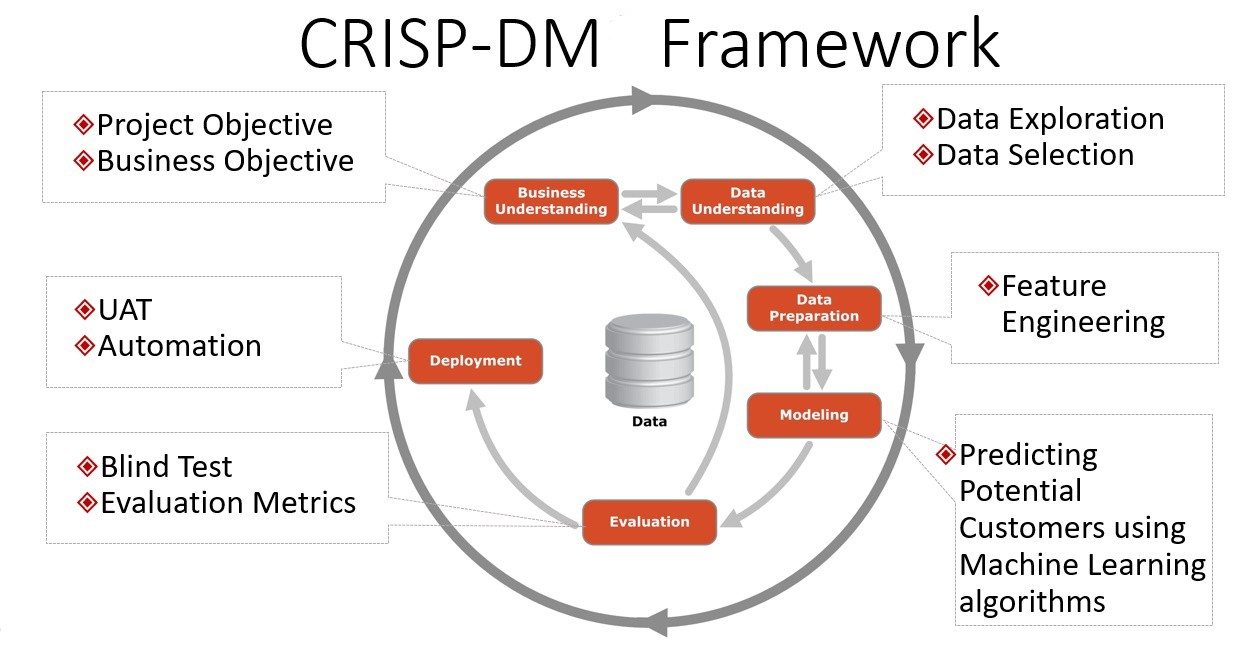
\includegraphics{crispdm.jpeg}
\caption{Diagrama da CRISP-DM}
\end{figure}

\hypertarget{fase-1---entendimento-do-neguxf3cio}{%
\section{Fase 1 - Entendimento do
Negócio}\label{fase-1---entendimento-do-neguxf3cio}}

\hypertarget{o-que-uxe9-o-sistema-nacional-de-puxf3s-graduauxe7uxe3o-contextualizauxe7uxe3o}{%
\subsection{O que é o Sistema Nacional de Pós-Graduação?
(Contextualização)}\label{o-que-uxe9-o-sistema-nacional-de-puxf3s-graduauxe7uxe3o-contextualizauxe7uxe3o}}

O Sistema de Avaliação da Pós-graduação foi implantado pela CAPES em
1976 e desde então vem cumprindo papel de fundamental importância para o
desenvolvimento da pós-graduação e da pesquisa científica e tecnológica
no Brasil. Abrange dois processos conduzidos por comissões de
consultores do mais alto nível, vinculados a instituições de ensino das
diferentes regiões do país: a Avaliação das Propostas de Cursos Novos e
a Avaliação dos Programas de Pós-graduação (Sucupira 2006).

A Avaliação das Propostas de Cursos Novos é parte do rito estabelecido
para a admissão de novos programas e cursos como integrantes do Sistema
Nacional de Pós-graduação, SNPG. Ao avaliar as propostas de cursos
novos, a CAPES verifica a qualidade de tais propostas e se elas atendem
ao padrão de qualidade requerido desse nível de formação. Os resultados
desse processo são encaminhados ao Conselho Nacional de Educação para
fundamentar a deliberação desse órgão sobre o reconhecimento dos novos
cursos.

A Avaliação dos Programas de Pós-graduação compreende os processos de
Acompanhamento Anual e de Avaliação Trienal do desempenho dos programas
e cursos que integram o Sistema Nacional de Pós-graduação, SNPG.

O Acompanhamento Anual é realizado no período compreendido entre os anos
de realização das avaliações trienais. Tem por objetivo o
estabelecimento de um diálogo entre a CAPES e as instituições promotoras
de cursos de mestrado e doutorado com vistas à orientação da atuação dos
programas de forma que possam elevar a qualidade de seu desempenho e
superar os problemas que eventualmente estejam a enfrentar - se possível
antes da Avaliação Trienal subseqüente. O Acompanhamento não implica na
atribuição de conceitos aos programas, mas apenas na apresentação de um
parecer com os comentários considerados pertinentes pela Comissão de
Área, e não enseja que seus resultados sejam contestados mediante a
apresentação de recursos ou pedidos de reconsideração.

A Avaliação Trienal é realizada ao final de cada triênio, sendo o ano de
sua realização estabelecido pela seqüência histórica do processo de
avaliação da CAPES. Os resultados da avaliação de cada programa são
apresentados na ``Ficha de Avaliação'' definida pelo CTC, de que
constam, no que se refere aos vários quesitos e itens avaliados, os
atributos a ele consignados, com os respectivos comentários e
justificativas da comissão avaliadora, e, ao final, o conceito
correspondente ao seu desempenho no triênio, na escala de 1 a 7 adotada.
Tais resultados podem ser contestados pelas instituições de ensino
mediante a apresentação de recurso contra a decisão inicial comunicada
pela CAPES e, uma vez homologados pelo Ministro da Educação, são válidos
até a homologação dos resultados da Avaliação Trienal subseqüente. Os
resultados da Avaliação Trienal realizada pela CAPES, além de indicarem
a qualidade do desempenho e a posição relativa de cada programa no
contexto de sua respectiva área, servem de referência para as decisões
dos órgãos governamentais de investimento na pesquisa e na pós-graduação
e fundamentam as deliberações do Conselho Nacional de Educação sobre
quais cursos de mestrado e de doutorado obterão, para vigência no
triênio seguinte, a renovação de seu ``reconhecimento''.

\hypertarget{a-unb-dentro-do-sistema-nacional-de-puxf3s-graduauxe7uxe3o-contextualizauxe7uxe3o}{%
\subsection{A UnB dentro do Sistema Nacional de Pós-Graduação
(Contextualização)}\label{a-unb-dentro-do-sistema-nacional-de-puxf3s-graduauxe7uxe3o-contextualizauxe7uxe3o}}

Historicamente, o desenvolvimento da ciência na UnB é realizado nas
unidades acadêmicas com apoio, acompanhamento e supervisão do Decanato
de Pesquisa e Pós-Graduação (DPP). A atuação do decanato promove todas
as áreas do conhecimento com o auxílio de diretorias específicas para
pesquisa, desenvolvimento institucional e inovação e iniciação
científica (UnB 2006).

Para estimular a pesquisa e a inovação e tornar a Universidade de
Brasília uma referência na área, foi criado, no início de 2017, o
Decanato de Pesquisa e Inovação (DPI). Com a mudança, o DPP passou a se
chamar Decanato de Pós-Graduação (DPG). A intenção é que as
pró-reitorias somem expertises em seus respectivos setores de atuação e
possam conduzir a UnB adiante na produção científica.

Editais próprios e de agências de fomento como CNPq, Capes e FAPDF são
responsáveis por financiar parte significativa das pesquisas na
Universidade. O DPG anuncia em sua página as publicações internas e as
principais chamadas públicas que podem beneficiar a comunidade
científica com a concessão de aportes financeiros, equipamentos, bolsas
e realização e participação em eventos científicos.

Algumas das principais definições estratégicas para o progresso da
ciência na UnB são realizadas no Conselho de Ensino, Pesquisa e Extensão
(Cepe), com apoio da Câmara de Pesquisa e Pós-Graduação (CPP). Essas
estruturas colegiadas permitem decisões democráticas com participação
ativa dos segmentos interessados.

De acordo com a plataforma sucupira, existem 97 programas em
funcionamento na Universidade de Brasília no momento. As notas por
programa se separam da seguinte maneira:

\begin{itemize}
\tightlist
\item
  5 programas com nota 7: Antropologia, Desenvolvimento Sustentável,
  Geologia, Matemática e Sociologia.
\item
  10 programas com nota 6: Geotecnia, Ciência Política, Ciências
  Biológicas (Biologia Molecular), Direito e outros.
\item
  18 programas com nota 5: Administração, Administração (pública),
  Bioética, Ciências animais, Ciências da informação, Ciências da saúde
  e outros.
\item
  46 programas com nota 4: Ensino de Ciências Ambientais em Rede
  Nacional, Agronegócios, Agronomia, Arquitetura E Urbanismo, Artes,
  Artes Cênicas, Biologia Animal, Biologia Microbiana e outros.
\end{itemize}

\hypertarget{fase-2---entendimento-dos-dados}{%
\section{Fase 2 - Entendimento dos
Dados}\label{fase-2---entendimento-dos-dados}}

\hypertarget{coleta-inicial-dos-dados}{%
\subsection{Coleta inicial dos dados}\label{coleta-inicial-dos-dados}}

Os arquivos json para análise foram fornecidos na plataforma unb.elattes
da UnB, que disponibiliza de forma acessível informações relevantes dos
programas avaliados. Os dados fornecem informações entre os anos de 2010
e 2019 (Fernandes and Sampaio 2011).

Perfil profissional dos docentes vinculados às pós-graduações

\begin{Shaded}
\begin{Highlighting}[]
\KeywordTok{file.info}\NormalTok{(}\StringTok{"Geotecnia/profile.json"}\NormalTok{)}
\end{Highlighting}
\end{Shaded}

\begin{verbatim}
##                          size isdir mode               mtime
## Geotecnia/profile.json 805404 FALSE  666 2019-08-30 19:29:28
##                                      ctime               atime exe
## Geotecnia/profile.json 2019-10-14 20:50:06 2019-10-14 20:50:06  no
\end{verbatim}

O arquivo profile.json apresenta dados sobre o perfil de todos os
docentes vinculados a programas de pós-graduação da UnB, entre 2010 e
2019. Esse arquivo foi fornecido pelos docentes responsáveis pela
disciplina.

Orientações de mestrado e doutorado realizadas pelos docentes vinculados
às pós-graduações

\begin{Shaded}
\begin{Highlighting}[]
\KeywordTok{file.info}\NormalTok{(}\StringTok{"Geotecnia/advise.json"}\NormalTok{)}
\end{Highlighting}
\end{Shaded}

\begin{verbatim}
##                         size isdir mode               mtime
## Geotecnia/advise.json 289779 FALSE  666 2019-08-30 19:29:28
##                                     ctime               atime exe
## Geotecnia/advise.json 2019-10-14 20:50:06 2019-10-14 20:50:06  no
\end{verbatim}

O arquivo advise.json apresenta dados sobre o orientações de mestrado e
doutorado feitas por todos os docentes vinculados a programas de
pós-graduação da UnB, entre 2010 e 2019. Esse arquivo foi fornecido
pelos docentes responsáveis pela disciplina.

Produção bibliográfica gerada pelos docentes vinculados às
pós-graduações

\begin{Shaded}
\begin{Highlighting}[]
\KeywordTok{file.info}\NormalTok{(}\StringTok{"Geotecnia/publication.json"}\NormalTok{)}
\end{Highlighting}
\end{Shaded}

\begin{verbatim}
##                              size isdir mode               mtime
## Geotecnia/publication.json 419637 FALSE  666 2019-08-30 19:29:28
##                                          ctime               atime exe
## Geotecnia/publication.json 2019-10-14 20:50:06 2019-10-14 20:50:06  no
\end{verbatim}

O arquivo publication.json apresenta dados sobre a produção
bibliográfica gerada por todos os docentes vinculados a programas de
pós-graduação da UnB, entre 2010 e 2019.

Agrupamento dos docentes conforme áreas de atuação

\begin{Shaded}
\begin{Highlighting}[]
\KeywordTok{file.info}\NormalTok{(}\StringTok{"Geotecnia/graph.json"}\NormalTok{)}
\end{Highlighting}
\end{Shaded}

\begin{verbatim}
##                      size isdir mode               mtime
## Geotecnia/graph.json 3392 FALSE  666 2019-08-30 19:29:28
##                                    ctime               atime exe
## Geotecnia/graph.json 2019-10-14 20:50:06 2019-10-14 20:50:06  no
\end{verbatim}

O arquivos graph.json de Geotecnia apresenta redes de colaboração na
co-autoria de artigos científicos, feitas entre os docentes vinculados a
programas de pós-graduação da UnB, entre 2010 e 2019.

\hypertarget{descriuxe7uxe3o-dos-dados}{%
\subsection{Descrição dos Dados}\label{descriuxe7uxe3o-dos-dados}}

Para ler, manipular, analisar e visualizar estes dados, serão utilizadas
as seguintes bibliotecas:

\begin{Shaded}
\begin{Highlighting}[]
\KeywordTok{library}\NormalTok{(tidyverse)}
\KeywordTok{library}\NormalTok{(jsonlite)}
\KeywordTok{library}\NormalTok{(listviewer)}
\KeywordTok{library}\NormalTok{(scales)}
\KeywordTok{library}\NormalTok{(dplyr)}
\KeywordTok{library}\NormalTok{(readxl)}
\KeywordTok{library}\NormalTok{(readr)}
\KeywordTok{library}\NormalTok{(readtext)}
\KeywordTok{library}\NormalTok{(ggplot2)}
\KeywordTok{library}\NormalTok{(igraph)}
\KeywordTok{library}\NormalTok{(knitr)}
\end{Highlighting}
\end{Shaded}

Com essas bibliotecas habilitadas será possível de responder e
determinar qual o volume de dados, a estrutura dos dados (tipos),
codificações usadas, entre outras atividades importantes para análise
dos dados.

Descrição dos dados do perfil

O arquivo profile.json, que contém dados que caracterizam o perfil
profissional de todos os docentes do grupo sob análise, podem ser lido
por meio do comando seguinte:

\begin{Shaded}
\begin{Highlighting}[]
\NormalTok{profile <-}\StringTok{ }\KeywordTok{fromJSON}\NormalTok{(}\StringTok{"Geotecnia/profile.json"}\NormalTok{)}
\end{Highlighting}
\end{Shaded}

A quantidade de docentes de Geotecnia sob análise é apresentada a
seguir.

\begin{Shaded}
\begin{Highlighting}[]
\KeywordTok{length}\NormalTok{(profile)}
\end{Highlighting}
\end{Shaded}

\begin{verbatim}
## [1] 12
\end{verbatim}

Para apresentar os dados que estão contido nos dados de perfil dos
docentes, vamos usar a função glimpse, da biblioteca dplyr, como ilustra
o código seguinte, que apresenta os atributos típicos que podem ser
obtidos relativamente a um pesquisador específico, o mais antigo docente
ainda em exercício na UnB a ter criado seu registro na plataforma
unb.elattes.

\begin{Shaded}
\begin{Highlighting}[]
\KeywordTok{glimpse}\NormalTok{(profile[[}\DecValTok{1}\NormalTok{]], }\DataTypeTok{width =} \DecValTok{30}\NormalTok{)}
\end{Highlighting}
\end{Shaded}

\begin{verbatim}
## List of 7
##  $ nome                  : chr "André Luís Brasil Cavalcante"
##  $ resumo_cv             : chr "André L. Brasil Cavalcante graduou-se em Engenharia Civil pela Universidade de Brasília em 1997, ocasião na qua"| __truncated__
##  $ areas_de_atuacao      :'data.frame':  4 obs. of  4 variables:
##   ..$ grande_area  : chr [1:4] "ENGENHARIAS" "ENGENHARIAS" "ENGENHARIAS" "ENGENHARIAS"
##   ..$ area         : chr [1:4] "Engenharia Civil" "Engenharia Civil" "Engenharia Civil" "Engenharia Mecânica"
##   ..$ sub_area     : chr [1:4] "Geotécnica" "Geotécnica" "Geotécnica" "Fenômenos de Transporte"
##   ..$ especialidade: chr [1:4] "Geotecnia Ambiental e Mineração" "Remediação de Áreas Contaminadas" "Obras de Terra e Enrocamento" "Princípios Variacionais e Métodos Numéricos"
##  $ endereco_profissional :List of 8
##   ..$ instituicao: chr "Universidade de Brasília"
##   ..$ orgao      : chr "ENC/FT/UNB"
##   ..$ unidade    : chr ""
##   ..$ DDD        : chr "61"
##   ..$ telefone   : chr "31071269"
##   ..$ bairro     : chr "ASA NORTE"
##   ..$ cep        : chr "70910900"
##   ..$ cidade     : chr "Brasília"
##  $ producao_bibiografica :List of 6
##   ..$ ARTIGO_ACEITO                         :'data.frame':   2 obs. of  10 variables:
##   .. ..$ natureza        : chr [1:2] "NAO_INFORMADO" "NAO_INFORMADO"
##   .. ..$ titulo          : chr [1:2] "The Iota-Delta Function as an Alternative to Boolean Formalism" "On the Iota-Delta Function: Universality in Turing Machines' Representation"
##   .. ..$ periodico       : chr [1:2] "INTERNATIONAL JOURNAL OF FOUNDATIONS OF COMPUTER SCIENCE" "JOURNAL OF COMPUTER AND SYSTEM SCIENCES"
##   .. ..$ ano             : chr [1:2] "2018" "2018"
##   .. ..$ volume          : chr [1:2] "" ""
##   .. ..$ issn            : chr [1:2] "01290541" "00220000"
##   .. ..$ paginas         : chr [1:2] " - " " - "
##   .. ..$ doi             : chr [1:2] "" ""
##   .. ..$ autores         :List of 2
##   .. ..$ autores-endogeno:List of 2
##   ..$ CAPITULO_DE_LIVRO                     :'data.frame':   5 obs. of  13 variables:
##   .. ..$ tipo                    : chr [1:5] "Capítulo de livro publicado" "Capítulo de livro publicado" "Capítulo de livro publicado" "Capítulo de livro publicado" ...
##   .. ..$ titulo_do_capitulo      : chr [1:5] "Modelos teóricos de infiltração em meios porosos: equação de Richards e suas aplicações" "Energy and Reliability Applied to Continuous Flight Auger Pilings - The SCCAP Methodology" "Cellular Automata for Modeling Transport Phenomena in Porous Media" "Tomografias computadorizadas e análises numéricas aplicadas à caracterização da estrutura porosa de solos não saturados" ...
##   .. ..$ titulo_do_livro         : chr [1:5] "Tópicos sobre infiltração: teoria e prática aplicadas a solos tropicais" "Proceedings of the 18th International Conference on Soil Mechanics and Geotechnical Engineering. Challenges and"| __truncated__ "Numerical Methods in Geotechnical Engineering" "Solos não saturados no contexto geotécnico" ...
##   .. ..$ ano                     : chr [1:5] "2012" "2013" "2014" "2015" ...
##   .. ..$ doi                     : chr [1:5] "" "" "10.1201/b17017-190" "" ...
##   .. ..$ pais_de_publicacao      : chr [1:5] "Brasil" "França" "Brasil" "Brasil" ...
##   .. ..$ isbn                    : chr [1:5] "9788560313419" "9782859784775" "9781138001466" "9788567950037" ...
##   .. ..$ nome_da_editora         : chr [1:5] "José Camapum de Carvalho, Gilson de Farias Neves Gitirana Junior, Eufrosina Terezinha Leão Carvalho" "Presses des Ponts" "Routledge Taylor & Francis Group" "ABMS" ...
##   .. ..$ numero_da_edicao_revisao: chr [1:5] "1" "1" "1" "1" ...
##   .. ..$ organizadores           : chr [1:5] "José Camapum de Carvalho; Gilson de Farias Neves Gitirana Junior, Eufrosina Terezinha Leão Carvalho" "Pierre Delage, Jacques Desrues, Roger Frank, Alain Puech, François Schlosser" "Michael A. Hicks, Ronald B.J. Brinkgreve, Alexander Rohe" "José Camapum de Carvalho, Gilson de Farias Neves Gitirana Junior, Sandro Lemos Machado, Márcia Maria dos Anjos "| __truncated__ ...
##   .. ..$ paginas                 : chr [1:5] "249 - 268" "2807 - 2810" "1073 - 1077" "531 - 553" ...
##   .. ..$ autores                 :List of 5
##   .. ..$ autores-endogeno        :List of 5
##   ..$ DEMAIS_TIPOS_DE_PRODUCAO_BIBLIOGRAFICA:'data.frame':   1 obs. of  9 variables:
##   .. ..$ natureza          : chr "Artigo Completo Publicado no Periódico arXiv"
##   .. ..$ titulo            : chr "Continuum versus Discrete: A Physically Interpretable General Rule for Cellular Automata by means of Modular Arithmetic"
##   .. ..$ ano               : chr "2012"
##   .. ..$ pais_de_publicacao: chr "Estados Unidos"
##   .. ..$ editora           : chr "arXiv"
##   .. ..$ doi               : chr ""
##   .. ..$ numero_de_paginas : chr "37"
##   .. ..$ autores           :List of 1
##   .. ..$ autores-endogeno  :List of 1
##   ..$ EVENTO                                :'data.frame':   68 obs. of  11 variables:
##   .. ..$ natureza        : chr [1:68] "COMPLETO" "RESUMO" "COMPLETO" "COMPLETO" ...
##   .. ..$ titulo          : chr [1:68] "Cálculo Probabilístico do Fator de Segurança em Projetos de Barragens de Rejeitos" "Modelagem Matemática da Contaminação de Rios, Utilizando o Microsoft Excel" "Modelagem Laboratorial e Numérica de Transporte de Contaminantes no Aterro Jóquei Clube no DF" "Riscos Associados aos Projetos de Barragens de Rejeito" ...
##   .. ..$ nome_do_evento  : chr [1:68] "XII Congresso Nacional de Geotecnia" "VI Simpósio Inovação no Ensino Superior" "COBRAMSEG 2010: Congresso Brasileiro de Mecânica dos Solos e Engenharia Geotécnica" "COBRAMSEG 2010: Congresso Brasileiro de Mecânica dos Solos e Engenharia Geotécnica" ...
##   .. ..$ ano_do_trabalho : chr [1:68] "2010" "2010" "2010" "2010" ...
##   .. ..$ pais_do_evento  : chr [1:68] "Portugal" "Brasil" "Brasil" "Brasil" ...
##   .. ..$ cidade_do_evento: chr [1:68] "Guimarães" "Brasília" "Gramado, RS" "Gramado, RS" ...
##   .. ..$ doi             : chr [1:68] "" "" "" "" ...
##   .. ..$ classificacao   : chr [1:68] "NACIONAL" "REGIONAL" "NACIONAL" "NACIONAL" ...
##   .. ..$ paginas         : chr [1:68] "1 - 8" "1 - 1" "1 - 8" "1 - 7" ...
##   .. ..$ autores         :List of 68
##   .. ..$ autores-endogeno:List of 68
##   ..$ LIVRO                                 :'data.frame':   1 obs. of  13 variables:
##   .. ..$ titulo                  : chr "Anais do Simpósio de Prática de Engenharia Geotécnica na Região Centro Oeste (GEOCENTRO 2017)"
##   .. ..$ ano                     : chr "2017"
##   .. ..$ tipo                    : chr "LIVRO_ORGANIZADO_OU_EDICAO"
##   .. ..$ natureza                : chr "ANAIS"
##   .. ..$ pais_de_publicacao      : chr "Brasil"
##   .. ..$ isbn                    : chr "9788567950051"
##   .. ..$ doi                     : chr ""
##   .. ..$ nome_da_editora         : chr "ABMS"
##   .. ..$ numero_da_edicao_revisao: chr "1"
##   .. ..$ numero_de_paginas       : chr "854"
##   .. ..$ numero_de_volumes       : chr "1"
##   .. ..$ autores                 :List of 1
##   .. ..$ autores-endogeno        :List of 1
##   ..$ PERIODICO                             :'data.frame':   31 obs. of  10 variables:
##   .. ..$ natureza        : chr [1:31] "COMPLETO" "COMPLETO" "COMPLETO" "COMPLETO" ...
##   .. ..$ titulo          : chr [1:31] "Lagrange's Inversion Theorem and Infiltration" "On Modelling Coninuous Flight Auger Pilings by means of Energy" "On Modelling Coninuous Flight Auger Pilings by means of Energy" "On Modeling Tailings Deposition: Analytical and Numerical Methods" ...
##   .. ..$ periodico       : chr [1:31] "World Academy of Science, Engineering and Technology (Online)" "International Journal of Science and Engineering Investigations" "International Journal of Science and Engineering Investigations" "International Journal of Science and Engineering Investigations" ...
##   .. ..$ ano             : chr [1:31] "2012" "2012" "2012" "2012" ...
##   .. ..$ volume          : chr [1:31] "6" "1" "01" "1" ...
##   .. ..$ issn            : chr [1:31] "20103778" "22518843" "22518843" "22518843" ...
##   .. ..$ paginas         : chr [1:31] "388 - 393" "11 - 16" "11 - 16" "64 - 70" ...
##   .. ..$ doi             : chr [1:31] "" "" "" "" ...
##   .. ..$ autores         :List of 31
##   .. ..$ autores-endogeno:List of 31
##  $ orientacoes_academicas:List of 8
##   ..$ ORIENTACAO_CONCLUIDA_DOUTORADO              :'data.frame': 5 obs. of  13 variables:
##   .. ..$ natureza                   : chr [1:5] "Tese de doutorado" "Tese de doutorado" "Tese de doutorado" "Tese de doutorado" ...
##   .. ..$ titulo                     : chr [1:5] "Concepção e Validaçao de um Modelo Matemático-digital para o Meio Poroso por Meio de Microtomografia, Autômatos"| __truncated__ "Aspectos Geotécnicos e e Ambientais para a Disposição Adequada de Lodo de Esgoto" "Aplicação da Lógica Fuzzy no Controle do Desempenho de Estacas Hélice Contínua" "Estudo Comparativo da Mobilidade de Contaminantes Inorgânicos em Solos Lateríticos e Não Lateríticos" ...
##   .. ..$ ano                        : chr [1:5] "2014" "2014" "2016" "2016" ...
##   .. ..$ id_lattes_aluno            : chr [1:5] "1853213451758913" "4994189165685449" "5372672441111608" "3289800404391423" ...
##   .. ..$ nome_aluno                 : chr [1:5] "Luan Carlos de S.M. Ozelim" "Leonardo Ramos da Silveira" "Mylane Viana Hortegal" "Renata Conciani" ...
##   .. ..$ instituicao                : chr [1:5] "Universidade de Brasília" "Universidade de Brasília" "Universidade de Brasília" "Universidade de Brasília" ...
##   .. ..$ curso                      : chr [1:5] "Geotecnia" "Geotecnia" "Geotecnia" "Geotecnia" ...
##   .. ..$ codigo_do_curso            : chr [1:5] "51500329" "51500329" "51500329" "51500329" ...
##   .. ..$ bolsa                      : chr [1:5] "SIM" "SIM" "SIM" "SIM" ...
##   .. ..$ agencia_financiadora       : chr [1:5] "Conselho Nacional de Desenvolvimento Científico e Tecnológico" "Conselho Nacional de Desenvolvimento Científico e Tecnológico" "Coordenação de Aperfeiçoamento de Pessoal de Nível Superior" "Conselho Nacional de Desenvolvimento Científico e Tecnológico" ...
##   .. ..$ codigo_agencia_financiadora: chr [1:5] "002200000000" "002200000000" "045000000000" "002200000000" ...
##   .. ..$ nome_orientadores          :List of 5
##   .. ..$ id_lattes_orientadores     :List of 5
##   ..$ ORIENTACAO_CONCLUIDA_MESTRADO               :'data.frame': 15 obs. of  13 variables:
##   .. ..$ natureza                   : chr [1:15] "Dissertação de mestrado" "Dissertação de mestrado" "Dissertação de mestrado" "Dissertação de mestrado" ...
##   .. ..$ titulo                     : chr [1:15] "Modelagem Multidimensional de Transporte de Contaminantes Inorgânicos em Solos Tropicais Lateríticos" "Estudo de Barreiras de Solo Compactado para Retenção de Contaminantes" "Análise do Transporte Multiespécies do Lixiviado de Moravia/Colômbia por meio de Ensaios em Coluna em Escala de"| __truncated__ "Transporte de Contaminantes Inorgânicos em Solos Tropicais Lateríticos: Abordagem com Cálculo Fracionário" ...
##   .. ..$ ano                        : chr [1:15] "2011" "2011" "2013" "2013" ...
##   .. ..$ id_lattes_aluno            : chr [1:15] "" "3289800404391423" "" "1811065164099319" ...
##   .. ..$ nome_aluno                 : chr [1:15] "Juan Fernando Díaz-Sánchez" "Renata Conciani" "Orly Tatiana Castaneda Rojas" "Ricardo Mendonça de Moraes" ...
##   .. ..$ instituicao                : chr [1:15] "Universidade de Brasília" "Universidade de Brasília" "Universidade de Brasília" "Universidade de Brasília" ...
##   .. ..$ curso                      : chr [1:15] "Geotecnia" "Geotecnia" "Geotecnia" "Geotecnia" ...
##   .. ..$ codigo_do_curso            : chr [1:15] "51500329" "51500329" "51500329" "51500329" ...
##   .. ..$ bolsa                      : chr [1:15] "SIM" "SIM" "SIM" "SIM" ...
##   .. ..$ agencia_financiadora       : chr [1:15] "Conselho Nacional de Desenvolvimento Científico e Tecnológico" "Conselho Nacional de Desenvolvimento Científico e Tecnológico" "Conselho Nacional de Desenvolvimento Científico e Tecnológico" "Conselho Nacional de Desenvolvimento Científico e Tecnológico" ...
##   .. ..$ codigo_agencia_financiadora: chr [1:15] "002200000000" "002200000000" "002200000000" "002200000000" ...
##   .. ..$ nome_orientadores          :List of 15
##   .. ..$ id_lattes_orientadores     :List of 15
##   ..$ ORIENTACAO_CONCLUIDA_POS_DOUTORADO          :'data.frame': 1 obs. of  13 variables:
##   .. ..$ natureza                   : chr "Supervisão de pós-doutorado"
##   .. ..$ titulo                     : chr ""
##   .. ..$ ano                        : chr "2017"
##   .. ..$ id_lattes_aluno            : chr ""
##   .. ..$ nome_aluno                 : chr "Luan Carlos de Sena Monteiro Ozelim"
##   .. ..$ instituicao                : chr "Universidade de Brasília"
##   .. ..$ curso                      : chr ""
##   .. ..$ codigo_do_curso            : chr ""
##   .. ..$ bolsa                      : chr "SIM"
##   .. ..$ agencia_financiadora       : chr "Conselho Nacional de Desenvolvimento Científico e Tecnológico"
##   .. ..$ codigo_agencia_financiadora: chr "002200000000"
##   .. ..$ nome_orientadores          :List of 1
##   .. ..$ id_lattes_orientadores     :List of 1
##   ..$ ORIENTACAO_EM_ANDAMENTO_DOUTORADO           :'data.frame': 6 obs. of  13 variables:
##   .. ..$ natureza                   : chr [1:6] "Tese de doutorado" "Tese de doutorado" "Tese de doutorado" "Tese de doutorado" ...
##   .. ..$ titulo                     : chr [1:6] "Avaliação do Fluxo de Contaminantes em Sistemas de Drenagem construídos com Materiais Alternativos." "Modelagem do Fluxo saturado e não saturado em condições de colapso e expansão" "Análise hidromecânica acoplada transiente do fenômeno de centrifugação em meios porosos não saturados" "Consequência das Mudanças Climáticas no Transporte de Contaminantes em Águas Subterrâneas" ...
##   .. ..$ ano                        : chr [1:6] "2014" "2016" "2017" "2017" ...
##   .. ..$ id_lattes_aluno            : chr [1:6] "" "9492644429017937" "6392971663534518" "" ...
##   .. ..$ nome_aluno                 : chr [1:6] "Silvana Fava Marchezini" "Lucas Parreira de Faria Borges" "Mateus Bezerra Alves da Costa" "Eliu James Carbajal Salinas" ...
##   .. ..$ instituicao                : chr [1:6] "Universidade de Brasília" "Universidade de Brasília" "Universidade de Brasília" "Universidade de Brasília" ...
##   .. ..$ curso                      : chr [1:6] "Geotecnia" "Geotecnia" "Geotecnia" "Geotecnia" ...
##   .. ..$ codigo_do_curso            : chr [1:6] "51500329" "51500329" "51500329" "51500329" ...
##   .. ..$ bolsa                      : chr [1:6] "SIM" "SIM" "SIM" "SIM" ...
##   .. ..$ agencia_financiadora       : chr [1:6] "Conselho Nacional de Desenvolvimento Científico e Tecnológico" "Conselho Nacional de Desenvolvimento Científico e Tecnológico" "Conselho Nacional de Desenvolvimento Científico e Tecnológico" "Conselho Nacional de Desenvolvimento Científico e Tecnológico" ...
##   .. ..$ codigo_agencia_financiadora: chr [1:6] "002200000000" "002200000000" "002200000000" "002200000000" ...
##   .. ..$ nome_orientadores          :List of 6
##   .. ..$ id_lattes_orientadores     :List of 6
##   ..$ ORIENTACAO_EM_ANDAMENTO_GRADUACAO           :'data.frame': 2 obs. of  13 variables:
##   .. ..$ natureza                   : chr [1:2] "Trabalho de conclusão de curso de graduação" "Trabalho de conclusão de curso de graduação"
##   .. ..$ titulo                     : chr [1:2] "Experimento de Fluxo em Meio Poroso Artificial Gerado por Impressão 3D" "Estudo sobre Sorção Não Linear em Solos Lateríticos"
##   .. ..$ ano                        : chr [1:2] "2017" "2017"
##   .. ..$ id_lattes_aluno            : chr [1:2] "" ""
##   .. ..$ nome_aluno                 : chr [1:2] "Nicholas Veres Barros" "Dhara Vieira Alcântara"
##   .. ..$ instituicao                : chr [1:2] "Universidade de Brasília" "Universidade de Brasília"
##   .. ..$ curso                      : chr [1:2] "Engenharia Civil" "Engenharia Civil"
##   .. ..$ codigo_do_curso            : chr [1:2] "60070293" "60070293"
##   .. ..$ bolsa                      : chr [1:2] "NAO" "NAO"
##   .. ..$ agencia_financiadora       : chr [1:2] "" ""
##   .. ..$ codigo_agencia_financiadora: chr [1:2] "" ""
##   .. ..$ nome_orientadores          :List of 2
##   .. ..$ id_lattes_orientadores     :List of 2
##   ..$ ORIENTACAO_EM_ANDAMENTO_INICIACAO_CIENTIFICA:'data.frame': 6 obs. of  13 variables:
##   .. ..$ natureza                   : chr [1:6] "Iniciação Científica" "Iniciação Científica" "Iniciação Científica" "Iniciação Científica" ...
##   .. ..$ titulo                     : chr [1:6] "Fluxo de Água em Meio Poroso Artificial Gerado por Impressão 3D" "Proposta de Concepção de Ensaio de Permeabilidade de Grandes Dimensões" "Transporte de Contaminantes em Barragens de Rejeitos aplicando Transformações Conformes" "Proposta de Concepção de Modelo Físico para Colchão Drenante com Material Alternativo: Escória de Aciaria" ...
##   .. ..$ ano                        : chr [1:6] "2017" "2017" "2017" "2017" ...
##   .. ..$ id_lattes_aluno            : chr [1:6] "" "" "" "" ...
##   .. ..$ nome_aluno                 : chr [1:6] "Nicholas Veres Barros" "Thália Raelly de Lima Meneses Romeiro" "André Luís de Alcântara Ramos" "Alexandre Rodarte Vieira de Sousa" ...
##   .. ..$ instituicao                : chr [1:6] "Universidade de Brasília" "Universidade de Brasília" "Universidade de Brasília" "Universidade de Brasília" ...
##   .. ..$ curso                      : chr [1:6] "Engenharia Civil" "Engenharia Civil" "Engenharia Civil" "Engenharia Civil" ...
##   .. ..$ codigo_do_curso            : chr [1:6] "60070293" "60070293" "60070293" "60070293" ...
##   .. ..$ bolsa                      : chr [1:6] "SIM" "NAO" "SIM" "NAO" ...
##   .. ..$ agencia_financiadora       : chr [1:6] "Fundação de Apoio à Pesquisa do Distrito Federal" "" "Conselho Nacional de Desenvolvimento Científico e Tecnológico" "" ...
##   .. ..$ codigo_agencia_financiadora: chr [1:6] "786500000001" "" "002200000000" "" ...
##   .. ..$ nome_orientadores          :List of 6
##   .. ..$ id_lattes_orientadores     :List of 6
##   ..$ ORIENTACAO_EM_ANDAMENTO_MESTRADO            :'data.frame': 3 obs. of  13 variables:
##   .. ..$ natureza                   : chr [1:3] "Dissertação de mestrado" "Dissertação de mestrado" "Dissertação de mestrado"
##   .. ..$ titulo                     : chr [1:3] "Modelagem fracionária de fluxo de água em meio poroso não saturado" "Modelagem Probabilística do Potencial de Contaminação para uma Área de Disposição Inadequada de Resíduos Sólidos" "Estudo e Avaliação de Técnicas de Remediação para uma Região Potencialmente Contaminada"
##   .. ..$ ano                        : chr [1:3] "2017" "2018" "2018"
##   .. ..$ id_lattes_aluno            : chr [1:3] "" "" ""
##   .. ..$ nome_aluno                 : chr [1:3] "Pedro Victor Serra Mascarenhas" "Mariana dos Santos Diniz" "Felipe Leite Nisiyama"
##   .. ..$ instituicao                : chr [1:3] "Universidade de Brasília" "Universidade de Brasília" "Universidade de Brasília"
##   .. ..$ curso                      : chr [1:3] "Geotecnia" "Geotecnia" "Geotecnia"
##   .. ..$ codigo_do_curso            : chr [1:3] "51500329" "51500329" "51500329"
##   .. ..$ bolsa                      : chr [1:3] "SIM" "SIM" "SIM"
##   .. ..$ agencia_financiadora       : chr [1:3] "Conselho Nacional de Desenvolvimento Científico e Tecnológico" "Conselho Nacional de Desenvolvimento Científico e Tecnológico" "Conselho Nacional de Desenvolvimento Científico e Tecnológico"
##   .. ..$ codigo_agencia_financiadora: chr [1:3] "002200000000" "002200000000" "002200000000"
##   .. ..$ nome_orientadores          :List of 3
##   .. ..$ id_lattes_orientadores     :List of 3
##   ..$ OUTRAS_ORIENTACOES_CONCLUIDAS               :'data.frame': 57 obs. of  13 variables:
##   .. ..$ natureza                   : chr [1:57] "INICIACAO_CIENTIFICA" "INICIACAO_CIENTIFICA" "INICIACAO_CIENTIFICA" "TRABALHO_DE_CONCLUSAO_DE_CURSO_GRADUACAO" ...
##   .. ..$ titulo                     : chr [1:57] "Ensaios laboratoriais em geotecnia e aplicações da geometria fractal" "Ensaios laboratoriais em geotecnia e aplicações em lógica fuzzy" "Ensaios laboratoriais em geotecnia e aplicações dos autômatos celulares" "Asfalto Permeável para Solução de Problemas com Enchentes nas Cidades." ...
##   .. ..$ ano                        : chr [1:57] "2010" "2010" "2010" "2010" ...
##   .. ..$ id_lattes_aluno            : chr [1:57] "" "" "" "" ...
##   .. ..$ nome_aluno                 : chr [1:57] "Pedro Henrique Lopes Batista" "Cristiano Nascimento Gouveia" "Diego Abreu Lemos" "Araujo, C. & Ribeiro, N.N." ...
##   .. ..$ instituicao                : chr [1:57] "Universidade Católica de Brasília" "Universidade Católica de Brasília" "Universidade Católica de Brasília" "Universidade Católica de Brasília" ...
##   .. ..$ curso                      : chr [1:57] "Engenharia Civil" "Engenharia Civil" "Engenharia Civil" "Engenharia Ambiental" ...
##   .. ..$ codigo_do_curso            : chr [1:57] "90000020" "90000020" "90000020" "90000022" ...
##   .. ..$ bolsa                      : chr [1:57] "SIM" "SIM" "NAO" "NAO" ...
##   .. ..$ agencia_financiadora       : chr [1:57] "Universidade Católica de Brasília" "Universidade Católica de Brasília" "" "" ...
##   .. ..$ codigo_agencia_financiadora: chr [1:57] "001000000998" "001000000998" "" "" ...
##   .. ..$ nome_orientadores          :List of 57
##   .. ..$ id_lattes_orientadores     :List of 57
##  $ senioridade           : chr "8"
\end{verbatim}

Uma breve inspeção visual dos atributos anteriormente apresentados
permite inferir que o pesquisador sob análise pode ser inferir que o
professor da área da engaranharia por formação, tendo geotécnica e
fenômenos de transporte como sua subárea, especialidades em Geotecnia
Ambiental e Mineração e Remediação de Áreas Contaminadas e atualmente
trabalha no campus Darcy Ribeiro da UnB com uma senioridade de 8.

Descrição dos dados de orientações

Carregando os dados do arquivo de orientação de geotecnia, podemos as
seguintes descrições:

\begin{Shaded}
\begin{Highlighting}[]
\NormalTok{advise <-}\StringTok{ }\KeywordTok{fromJSON}\NormalTok{(}\StringTok{"Geotecnia/advise.json"}\NormalTok{)}
\end{Highlighting}
\end{Shaded}

Os tipos de orientação que estarão sob análise:

\begin{Shaded}
\begin{Highlighting}[]
\KeywordTok{names}\NormalTok{(advise)}
\end{Highlighting}
\end{Shaded}

\begin{verbatim}
## [1] "ORIENTACAO_EM_ANDAMENTO_DE_POS_DOUTORADO"    
## [2] "ORIENTACAO_EM_ANDAMENTO_DOUTORADO"           
## [3] "ORIENTACAO_EM_ANDAMENTO_MESTRADO"            
## [4] "ORIENTACAO_EM_ANDAMENTO_GRADUACAO"           
## [5] "ORIENTACAO_EM_ANDAMENTO_INICIACAO_CIENTIFICA"
## [6] "ORIENTACAO_CONCLUIDA_POS_DOUTORADO"          
## [7] "ORIENTACAO_CONCLUIDA_DOUTORADO"              
## [8] "ORIENTACAO_CONCLUIDA_MESTRADO"               
## [9] "OUTRAS_ORIENTACOES_CONCLUIDAS"
\end{verbatim}

O período no qual será feita a análise:

\begin{Shaded}
\begin{Highlighting}[]
\KeywordTok{names}\NormalTok{(advise}\OperatorTok{$}\NormalTok{ORIENTACAO_CONCLUIDA_DOUTORADO)}
\end{Highlighting}
\end{Shaded}

\begin{verbatim}
##  [1] "2010" "2011" "2012" "2013" "2014" "2015" "2016" "2017" "2018" "2019"
\end{verbatim}

A quantidade de orientações de doutorado concluídas em um ano específico
(ex. 2016)

\begin{Shaded}
\begin{Highlighting}[]
\KeywordTok{length}\NormalTok{(advise}\OperatorTok{$}\NormalTok{ORIENTACAO_CONCLUIDA_DOUTORADO}\OperatorTok{$}\StringTok{`}\DataTypeTok{2016}\StringTok{`}\OperatorTok{$}\NormalTok{natureza)}
\end{Highlighting}
\end{Shaded}

\begin{verbatim}
## [1] 14
\end{verbatim}

Quais os cursos que mais contribuíram com teses concluídas em doutorado
em um ano específico (ex. 2017):

\begin{Shaded}
\begin{Highlighting}[]
\KeywordTok{head}\NormalTok{(}\KeywordTok{sort}\NormalTok{(}
  \KeywordTok{table}\NormalTok{(advise}\OperatorTok{$}\NormalTok{ORIENTACAO_CONCLUIDA_DOUTORADO}\OperatorTok{$}\StringTok{`}\DataTypeTok{2017}\StringTok{`}\OperatorTok{$}\NormalTok{curso),}
  \DataTypeTok{decreasing =} \OtherTok{TRUE}
\NormalTok{), }\DecValTok{10}\NormalTok{)}
\end{Highlighting}
\end{Shaded}

\begin{verbatim}
## Geotecnia 
##        11
\end{verbatim}

Quais os cursos que mais contribuíram com teses concluídas em mestrado
em um ano específico (ex. 2017):

\begin{Shaded}
\begin{Highlighting}[]
\KeywordTok{head}\NormalTok{(}\KeywordTok{sort}\NormalTok{(}
  \KeywordTok{table}\NormalTok{(advise}\OperatorTok{$}\NormalTok{ORIENTACAO_CONCLUIDA_MESTRADO}\OperatorTok{$}\StringTok{`}\DataTypeTok{2017}\StringTok{`}\OperatorTok{$}\NormalTok{curso),}
  \DataTypeTok{decreasing =} \OtherTok{TRUE}
\NormalTok{), }\DecValTok{10}\NormalTok{)}
\end{Highlighting}
\end{Shaded}

\begin{verbatim}
## 
##                                     Geotecnia 
##                                            13 
##        Programa de Pós-Graduação em Geotecnia 
##                                             2 
##                             Civil Engineering 
##                                             1 
##                         Mestrado em Geotecnia 
##                                             1 
## Mestrado Profissional em Engenharia Ambiental 
##                                             1
\end{verbatim}

Descrição dos dados de produção bibliográfica

Carregando os dados do arquivo de produção bibliográfica de Geotecnia,
podemos as seguintes descrições:

\begin{Shaded}
\begin{Highlighting}[]
\NormalTok{publication <-}\StringTok{ }\KeywordTok{fromJSON}\NormalTok{(}\StringTok{"Geotecnia/publication.json"}\NormalTok{)}
\end{Highlighting}
\end{Shaded}

Os tipos de produção bibliográfica a serem analisados nessa pesquisa:

\begin{Shaded}
\begin{Highlighting}[]
\KeywordTok{names}\NormalTok{(publication)}
\end{Highlighting}
\end{Shaded}

\begin{verbatim}
## [1] "PERIODICO"                             
## [2] "LIVRO"                                 
## [3] "CAPITULO_DE_LIVRO"                     
## [4] "TEXTO_EM_JORNAIS"                      
## [5] "EVENTO"                                
## [6] "ARTIGO_ACEITO"                         
## [7] "DEMAIS_TIPOS_DE_PRODUCAO_BIBLIOGRAFICA"
\end{verbatim}

Os tipos de informação que cada periódico contém em um ano especifico
(ex. 2012)

\begin{Shaded}
\begin{Highlighting}[]
\KeywordTok{names}\NormalTok{(publication}\OperatorTok{$}\NormalTok{PERIODICO}\OperatorTok{$}\StringTok{`}\DataTypeTok{2012}\StringTok{`}\NormalTok{)}
\end{Highlighting}
\end{Shaded}

\begin{verbatim}
##  [1] "natureza"         "titulo"           "periodico"       
##  [4] "ano"              "volume"           "issn"            
##  [7] "paginas"          "doi"              "autores"         
## [10] "autores-endogeno"
\end{verbatim}

Os periódicos com maior número de publicações para cada programa em um
determinado ano (ex. 2017):

\begin{Shaded}
\begin{Highlighting}[]
\KeywordTok{head}\NormalTok{(}\KeywordTok{sort}\NormalTok{(}\KeywordTok{table}\NormalTok{(publication}\OperatorTok{$}\NormalTok{PERIODICO}\OperatorTok{$}\StringTok{`}\DataTypeTok{2017}\StringTok{`}\OperatorTok{$}\NormalTok{periodico), }\DataTypeTok{decreasing =} \OtherTok{TRUE}\NormalTok{), }\DecValTok{10}\NormalTok{)}
\end{Highlighting}
\end{Shaded}

\begin{verbatim}
## 
##               Computational Particle Mechanics 
##                                              3 
##                                DYNA (MEDELLÍN) 
##                                              2 
##                      ENVIRONMENTAL GEOTECHNICS 
##                                              2 
##          International Journal of Geomechanics 
##                                              2 
##                                  SOILS & ROCKS 
##                                              2 
##                   Transportes (Rio de Janeiro) 
##                                              2 
##                    Boletim Goiano de Geografia 
##                                              1 
##                  CANADIAN GEOTECHNICAL JOURNAL 
##                                              1 
##                            Construção Magazine 
##                                              1 
## Electronic Journal of Geotechnical Engineering 
##                                              1
\end{verbatim}

As editoras com maior número de publicações para cada programa em um
determinado ano (ex. 2015):

\begin{Shaded}
\begin{Highlighting}[]
\KeywordTok{head}\NormalTok{(}\KeywordTok{sort}\NormalTok{(}
  \KeywordTok{table}\NormalTok{(publication}\OperatorTok{$}\NormalTok{LIVRO}\OperatorTok{$}\StringTok{`}\DataTypeTok{2015}\StringTok{`}\OperatorTok{$}\NormalTok{nome_da_editora),}
  \DataTypeTok{decreasing =} \OtherTok{TRUE}
\NormalTok{), }\DecValTok{10}\NormalTok{)}
\end{Highlighting}
\end{Shaded}

\begin{verbatim}
## ABMS 
##    1
\end{verbatim}

\hypertarget{anuxe1lise-exploratuxf3ria-dos-dados}{%
\subsection{Análise exploratória dos
dados}\label{anuxe1lise-exploratuxf3ria-dos-dados}}

A seguir será mostrado a análise exploratória dos dados nos datasets um
entendimento de qualidade mais profundo da relação estatística existente
para os objetivos do projeto.

\hypertarget{arquivo-perfil}{%
\subsubsection{Arquivo Perfil}\label{arquivo-perfil}}

Número de áreas de atuação cumulativo:

\begin{Shaded}
\begin{Highlighting}[]
\KeywordTok{sum}\NormalTok{(}\KeywordTok{sapply}\NormalTok{(profile, }\ControlFlowTok{function}\NormalTok{(x)}
  \KeywordTok{nrow}\NormalTok{(x}\OperatorTok{$}\NormalTok{areas_de_atuacao)))}
\end{Highlighting}
\end{Shaded}

\begin{verbatim}
## [1] 63
\end{verbatim}

Número de pessoas por áreas de atuação:

\begin{Shaded}
\begin{Highlighting}[]
\KeywordTok{table}\NormalTok{(}\KeywordTok{unlist}\NormalTok{(}\KeywordTok{sapply}\NormalTok{(profile, }\ControlFlowTok{function}\NormalTok{(x)}
  \KeywordTok{nrow}\NormalTok{(x}\OperatorTok{$}\NormalTok{areas_de_atuacao))))}
\end{Highlighting}
\end{Shaded}

\begin{verbatim}
## 
## 3 4 5 6 
## 1 2 2 7
\end{verbatim}

Número de pessoas por grande área:

\begin{Shaded}
\begin{Highlighting}[]
\KeywordTok{table}\NormalTok{(}\KeywordTok{unlist}\NormalTok{(}\KeywordTok{sapply}\NormalTok{(profile, }\ControlFlowTok{function}\NormalTok{(x)}
\NormalTok{  (x}\OperatorTok{$}\NormalTok{areas_de_atuacao}\OperatorTok{$}\NormalTok{grande_area))))}
\end{Highlighting}
\end{Shaded}

\begin{verbatim}
## 
## CIENCIAS_EXATAS_E_DA_TERRA CIENCIAS_SOCIAIS_APLICADAS 
##                          5                          2 
##                ENGENHARIAS 
##                         56
\end{verbatim}

Número de pessoas que produziram os específicos tipos de produção:

\begin{Shaded}
\begin{Highlighting}[]
\KeywordTok{table}\NormalTok{(}\KeywordTok{unlist}\NormalTok{(}\KeywordTok{sapply}\NormalTok{(profile, }\ControlFlowTok{function}\NormalTok{(x)}
  \KeywordTok{names}\NormalTok{(x}\OperatorTok{$}\NormalTok{producao_bibiografica))))}
\end{Highlighting}
\end{Shaded}

\begin{verbatim}
## 
##                          ARTIGO_ACEITO 
##                                      3 
##                      CAPITULO_DE_LIVRO 
##                                      9 
## DEMAIS_TIPOS_DE_PRODUCAO_BIBLIOGRAFICA 
##                                      4 
##                                 EVENTO 
##                                     12 
##                                  LIVRO 
##                                      6 
##                              PERIODICO 
##                                     12 
##                       TEXTO_EM_JORNAIS 
##                                      5
\end{verbatim}

Número de publicações por artigo aceito:

\begin{Shaded}
\begin{Highlighting}[]
\KeywordTok{sum}\NormalTok{(}\KeywordTok{sapply}\NormalTok{(profile, }\ControlFlowTok{function}\NormalTok{(x)}
  \KeywordTok{length}\NormalTok{(x}\OperatorTok{$}\NormalTok{producao_bibiografica}\OperatorTok{$}\NormalTok{ARTIGO_ACEITO}\OperatorTok{$}\NormalTok{ano)))}
\end{Highlighting}
\end{Shaded}

\begin{verbatim}
## [1] 4
\end{verbatim}

Número de publicações por capítulo de livro:

\begin{Shaded}
\begin{Highlighting}[]
\KeywordTok{sum}\NormalTok{(}\KeywordTok{sapply}\NormalTok{(profile, }\ControlFlowTok{function}\NormalTok{(x)}
  \KeywordTok{length}\NormalTok{(x}\OperatorTok{$}\NormalTok{producao_bibiografica}\OperatorTok{$}\NormalTok{CAPITULO_DE_LIVRO}\OperatorTok{$}\NormalTok{ano)))}
\end{Highlighting}
\end{Shaded}

\begin{verbatim}
## [1] 68
\end{verbatim}

Número de publicações por livro:

\begin{Shaded}
\begin{Highlighting}[]
\KeywordTok{sum}\NormalTok{(}\KeywordTok{sapply}\NormalTok{(profile, }\ControlFlowTok{function}\NormalTok{(x)}
  \KeywordTok{length}\NormalTok{(x}\OperatorTok{$}\NormalTok{producao_bibiografica}\OperatorTok{$}\NormalTok{LIVRO}\OperatorTok{$}\NormalTok{ano)))}
\end{Highlighting}
\end{Shaded}

\begin{verbatim}
## [1] 14
\end{verbatim}

Número de publicações por periódico:

\begin{Shaded}
\begin{Highlighting}[]
\KeywordTok{sum}\NormalTok{(}\KeywordTok{sapply}\NormalTok{(profile, }\ControlFlowTok{function}\NormalTok{(x)}
  \KeywordTok{length}\NormalTok{(x}\OperatorTok{$}\NormalTok{producao_bibiografica}\OperatorTok{$}\NormalTok{PERIODICO}\OperatorTok{$}\NormalTok{ano)))}
\end{Highlighting}
\end{Shaded}

\begin{verbatim}
## [1] 201
\end{verbatim}

Número de publicações por texto em jornais:

\begin{Shaded}
\begin{Highlighting}[]
\KeywordTok{sum}\NormalTok{(}\KeywordTok{sapply}\NormalTok{(profile, }\ControlFlowTok{function}\NormalTok{(x)}
  \KeywordTok{length}\NormalTok{(x}\OperatorTok{$}\NormalTok{producao_bibiografica}\OperatorTok{$}\NormalTok{TEXTO_EM_JORNAIS}\OperatorTok{$}\NormalTok{ano)))}
\end{Highlighting}
\end{Shaded}

\begin{verbatim}
## [1] 14
\end{verbatim}

Número de pessoas por quantitativo de produções por artigo aceito:

\begin{Shaded}
\begin{Highlighting}[]
\KeywordTok{table}\NormalTok{(}\KeywordTok{unlist}\NormalTok{(}\KeywordTok{sapply}\NormalTok{(profile, }\ControlFlowTok{function}\NormalTok{(x)}
  \KeywordTok{length}\NormalTok{(x}\OperatorTok{$}\NormalTok{producao_bibiografica}\OperatorTok{$}\NormalTok{ARTIGO_ACEITO}\OperatorTok{$}\NormalTok{ano))))}
\end{Highlighting}
\end{Shaded}

\begin{verbatim}
## 
## 0 1 2 
## 9 2 1
\end{verbatim}

Número de pessoas por quantitativo de produções por capítulo de livro:

\begin{Shaded}
\begin{Highlighting}[]
\KeywordTok{table}\NormalTok{(}\KeywordTok{unlist}\NormalTok{(}\KeywordTok{sapply}\NormalTok{(profile, }\ControlFlowTok{function}\NormalTok{(x)}
  \KeywordTok{length}\NormalTok{(x}\OperatorTok{$}\NormalTok{producao_bibiografica}\OperatorTok{$}\NormalTok{CAPITULO_DE_LIVRO}\OperatorTok{$}\NormalTok{ano))))}
\end{Highlighting}
\end{Shaded}

\begin{verbatim}
## 
##  0  1  2  5  6  8 38 
##  3  3  1  1  2  1  1
\end{verbatim}

Número de pessoas por quantitativo de produções por livro:

\begin{Shaded}
\begin{Highlighting}[]
\KeywordTok{table}\NormalTok{(}\KeywordTok{unlist}\NormalTok{(}\KeywordTok{sapply}\NormalTok{(profile, }\ControlFlowTok{function}\NormalTok{(x)}
  \KeywordTok{length}\NormalTok{(x}\OperatorTok{$}\NormalTok{producao_bibiografica}\OperatorTok{$}\NormalTok{LIVRO}\OperatorTok{$}\NormalTok{ano))))}
\end{Highlighting}
\end{Shaded}

\begin{verbatim}
## 
## 0 1 3 7 
## 6 4 1 1
\end{verbatim}

Número de pessoas por quantitativo de produções por periódico:

\begin{Shaded}
\begin{Highlighting}[]
\KeywordTok{table}\NormalTok{(}\KeywordTok{unlist}\NormalTok{(}\KeywordTok{sapply}\NormalTok{(profile, }\ControlFlowTok{function}\NormalTok{(x)}
  \KeywordTok{length}\NormalTok{(x}\OperatorTok{$}\NormalTok{producao_bibiografica}\OperatorTok{$}\NormalTok{PERIODICO}\OperatorTok{$}\NormalTok{ano))))}
\end{Highlighting}
\end{Shaded}

\begin{verbatim}
## 
##  3  5 14 15 26 27 31 32 
##  2  2  2  1  2  1  1  1
\end{verbatim}

Número de pessoas por quantitativo de produções por texto em jornais:

\begin{Shaded}
\begin{Highlighting}[]
\KeywordTok{table}\NormalTok{(}\KeywordTok{unlist}\NormalTok{(}\KeywordTok{sapply}\NormalTok{(profile, }\ControlFlowTok{function}\NormalTok{(x)}
  \KeywordTok{length}\NormalTok{(x}\OperatorTok{$}\NormalTok{producao_bibiografica}\OperatorTok{$}\NormalTok{TEXTO_EM_JORNAIS}\OperatorTok{$}\NormalTok{ano))))}
\end{Highlighting}
\end{Shaded}

\begin{verbatim}
## 
## 0 2 3 4 
## 7 2 2 1
\end{verbatim}

Número de produções de artigo aceito por ano:

\begin{Shaded}
\begin{Highlighting}[]
\KeywordTok{table}\NormalTok{(}\KeywordTok{unlist}\NormalTok{(}\KeywordTok{sapply}\NormalTok{(profile, }\ControlFlowTok{function}\NormalTok{(x)}
\NormalTok{  (x}\OperatorTok{$}\NormalTok{producao_bibiografica}\OperatorTok{$}\NormalTok{ARTIGO_ACEITO}\OperatorTok{$}\NormalTok{ano))))}
\end{Highlighting}
\end{Shaded}

\begin{verbatim}
## 
## 2014 2018 
##    1    3
\end{verbatim}

Número de produções de capítulo de livro por ano:

\begin{Shaded}
\begin{Highlighting}[]
\KeywordTok{table}\NormalTok{(}\KeywordTok{unlist}\NormalTok{(}\KeywordTok{sapply}\NormalTok{(profile, }\ControlFlowTok{function}\NormalTok{(x)}
\NormalTok{  (x}\OperatorTok{$}\NormalTok{producao_bibiografica}\OperatorTok{$}\NormalTok{CAPITULO_DE_LIVRO}\OperatorTok{$}\NormalTok{ano))))}
\end{Highlighting}
\end{Shaded}

\begin{verbatim}
## 
## 2012 2013 2014 2015 2016 2017 
##   33    1    3   11    2   18
\end{verbatim}

Número de produções de livro por ano:

\begin{Shaded}
\begin{Highlighting}[]
\KeywordTok{table}\NormalTok{(}\KeywordTok{unlist}\NormalTok{(}\KeywordTok{sapply}\NormalTok{(profile, }\ControlFlowTok{function}\NormalTok{(x)}
\NormalTok{  (x}\OperatorTok{$}\NormalTok{producao_bibiografica}\OperatorTok{$}\NormalTok{LIVRO}\OperatorTok{$}\NormalTok{ano))))}
\end{Highlighting}
\end{Shaded}

\begin{verbatim}
## 
## 2010 2011 2012 2014 2015 2016 2017 
##    2    1    3    1    1    2    4
\end{verbatim}

Número de produções de periódico por ano:

\begin{Shaded}
\begin{Highlighting}[]
\KeywordTok{table}\NormalTok{(}\KeywordTok{unlist}\NormalTok{(}\KeywordTok{sapply}\NormalTok{(profile, }\ControlFlowTok{function}\NormalTok{(x)}
\NormalTok{  (x}\OperatorTok{$}\NormalTok{producao_bibiografica}\OperatorTok{$}\NormalTok{PERIODICO}\OperatorTok{$}\NormalTok{ano))))}
\end{Highlighting}
\end{Shaded}

\begin{verbatim}
## 
## 2010 2011 2012 2013 2014 2015 2016 2017 2018 
##   20   11   21   27   27   32   30   26    7
\end{verbatim}

Número de produções de texto em jornais por ano:

\begin{Shaded}
\begin{Highlighting}[]
\KeywordTok{table}\NormalTok{(}\KeywordTok{unlist}\NormalTok{(}\KeywordTok{sapply}\NormalTok{(profile, }\ControlFlowTok{function}\NormalTok{(x)}
\NormalTok{  (x}\OperatorTok{$}\NormalTok{producao_bibiografica}\OperatorTok{$}\NormalTok{TEXTO_EM_JORNAIS}\OperatorTok{$}\NormalTok{ano))))}
\end{Highlighting}
\end{Shaded}

\begin{verbatim}
## 
## 2011 2012 2013 2014 2015 2016 
##    2    2    3    1    1    5
\end{verbatim}

Número de pessoas que realizaram diferentes tipos de orientações:

\begin{Shaded}
\begin{Highlighting}[]
\KeywordTok{length}\NormalTok{(}\KeywordTok{unlist}\NormalTok{(}\KeywordTok{sapply}\NormalTok{(profile, }\ControlFlowTok{function}\NormalTok{(x)}
  \KeywordTok{names}\NormalTok{(x}\OperatorTok{$}\NormalTok{orientacoes_academicas))))}
\end{Highlighting}
\end{Shaded}

\begin{verbatim}
## [1] 67
\end{verbatim}

Número de pessoas por tipo de orientação:

\begin{Shaded}
\begin{Highlighting}[]
\KeywordTok{table}\NormalTok{(}\KeywordTok{unlist}\NormalTok{(}\KeywordTok{sapply}\NormalTok{(profile, }\ControlFlowTok{function}\NormalTok{(x)}
  \KeywordTok{names}\NormalTok{(x}\OperatorTok{$}\NormalTok{orientacoes_academicas))))}
\end{Highlighting}
\end{Shaded}

\begin{verbatim}
## 
##               ORIENTACAO_CONCLUIDA_DOUTORADO 
##                                           11 
##                ORIENTACAO_CONCLUIDA_MESTRADO 
##                                           12 
##           ORIENTACAO_CONCLUIDA_POS_DOUTORADO 
##                                            4 
##            ORIENTACAO_EM_ANDAMENTO_DOUTORADO 
##                                           11 
##            ORIENTACAO_EM_ANDAMENTO_GRADUACAO 
##                                            1 
## ORIENTACAO_EM_ANDAMENTO_INICIACAO_CIENTIFICA 
##                                            6 
##             ORIENTACAO_EM_ANDAMENTO_MESTRADO 
##                                           10 
##                OUTRAS_ORIENTACOES_CONCLUIDAS 
##                                           12
\end{verbatim}

Número de orientações concluídas em mestrado:

\begin{Shaded}
\begin{Highlighting}[]
\KeywordTok{sum}\NormalTok{(}\KeywordTok{sapply}\NormalTok{(profile, }\ControlFlowTok{function}\NormalTok{(x)}
  \KeywordTok{length}\NormalTok{(x}\OperatorTok{$}\NormalTok{orientacoes_academicas}\OperatorTok{$}\NormalTok{ORIENTACAO_CONCLUIDA_MESTRADO}\OperatorTok{$}\NormalTok{ano)))}
\end{Highlighting}
\end{Shaded}

\begin{verbatim}
## [1] 153
\end{verbatim}

Número de orientações concluídas em doutorado:

\begin{Shaded}
\begin{Highlighting}[]
\KeywordTok{sum}\NormalTok{(}\KeywordTok{sapply}\NormalTok{(profile, }\ControlFlowTok{function}\NormalTok{(x)}
  \KeywordTok{length}\NormalTok{(}
\NormalTok{    x}\OperatorTok{$}\NormalTok{orientacoes_academicas}\OperatorTok{$}\NormalTok{ORIENTACAO_CONCLUIDA_DOUTORADO}\OperatorTok{$}\NormalTok{ano}
\NormalTok{  )))}
\end{Highlighting}
\end{Shaded}

\begin{verbatim}
## [1] 89
\end{verbatim}

Número de orientações concluídas em pós-doutorado:

\begin{Shaded}
\begin{Highlighting}[]
\KeywordTok{sum}\NormalTok{(}\KeywordTok{sapply}\NormalTok{(profile, }\ControlFlowTok{function}\NormalTok{(x)}
  \KeywordTok{length}\NormalTok{(}
\NormalTok{    x}\OperatorTok{$}\NormalTok{orientacoes_academicas}\OperatorTok{$}\NormalTok{ORIENTACAO_CONCLUIDA_POS_DOUTORADO}\OperatorTok{$}\NormalTok{ano}
\NormalTok{  )))}
\end{Highlighting}
\end{Shaded}

\begin{verbatim}
## [1] 6
\end{verbatim}

Número de pessoas por quantitativo de orientações concluídas em
mestrado:

\begin{Shaded}
\begin{Highlighting}[]
\KeywordTok{table}\NormalTok{(}\KeywordTok{unlist}\NormalTok{(}\KeywordTok{sapply}\NormalTok{(profile, }\ControlFlowTok{function}\NormalTok{(x)}
  \KeywordTok{length}\NormalTok{(x}\OperatorTok{$}\NormalTok{orientacoes_academicas}\OperatorTok{$}\NormalTok{ORIENTACAO_CONCLUIDA_MESTRADO}\OperatorTok{$}\NormalTok{ano))))}
\end{Highlighting}
\end{Shaded}

\begin{verbatim}
## 
##  6  7  8 10 11 12 13 15 19 25 
##  1  1  1  1  1  2  1  2  1  1
\end{verbatim}

Número de pessoas por quantitativo de orientações concluídas em
doutorado:

\begin{Shaded}
\begin{Highlighting}[]
\KeywordTok{table}\NormalTok{(}\KeywordTok{unlist}\NormalTok{(}\KeywordTok{sapply}\NormalTok{(profile, }\ControlFlowTok{function}\NormalTok{(x)}
  \KeywordTok{length}\NormalTok{(}
\NormalTok{    x}\OperatorTok{$}\NormalTok{orientacoes_academicas}\OperatorTok{$}\NormalTok{ORIENTACAO_CONCLUIDA_DOUTORADO}\OperatorTok{$}\NormalTok{ano}
\NormalTok{  ))))}
\end{Highlighting}
\end{Shaded}

\begin{verbatim}
## 
##  0  1  5  7  8  9 10 11 12 13 
##  1  1  2  1  2  1  1  1  1  1
\end{verbatim}

Número de pessoas por quantitativo de orientações concluídas em
pós-doutorado:

\begin{Shaded}
\begin{Highlighting}[]
\KeywordTok{table}\NormalTok{(}\KeywordTok{unlist}\NormalTok{(}\KeywordTok{sapply}\NormalTok{(profile, }\ControlFlowTok{function}\NormalTok{(x)}
  \KeywordTok{length}\NormalTok{(}
\NormalTok{    x}\OperatorTok{$}\NormalTok{orientacoes_academicas}\OperatorTok{$}\NormalTok{ORIENTACAO_CONCLUIDA_POS_DOUTORADO}\OperatorTok{$}\NormalTok{ano}
\NormalTok{  ))))}
\end{Highlighting}
\end{Shaded}

\begin{verbatim}
## 
## 0 1 2 
## 8 2 2
\end{verbatim}

Número de orientações em mestrado por ano:

\begin{Shaded}
\begin{Highlighting}[]
\KeywordTok{table}\NormalTok{(}\KeywordTok{unlist}\NormalTok{(}\KeywordTok{sapply}\NormalTok{(profile, }\ControlFlowTok{function}\NormalTok{(x)}
\NormalTok{  (x}\OperatorTok{$}\NormalTok{orientacoes_academicas}\OperatorTok{$}\NormalTok{ORIENTACAO_CONCLUIDA_MESTRADO}\OperatorTok{$}\NormalTok{ano))))}
\end{Highlighting}
\end{Shaded}

\begin{verbatim}
## 
## 2010 2011 2012 2013 2014 2015 2016 2017 2018 
##    8   19   20   21   16   20   25   19    5
\end{verbatim}

Número de orientações em doutorado por ano:

\begin{Shaded}
\begin{Highlighting}[]
\KeywordTok{table}\NormalTok{(}\KeywordTok{unlist}\NormalTok{(}\KeywordTok{sapply}\NormalTok{(profile, }\ControlFlowTok{function}\NormalTok{(x)}
\NormalTok{  (}
\NormalTok{    x}\OperatorTok{$}\NormalTok{orientacoes_academicas}\OperatorTok{$}\NormalTok{ORIENTACAO_CONCLUIDA_DOUTORADO}\OperatorTok{$}\NormalTok{ano}
\NormalTok{  ))))}
\end{Highlighting}
\end{Shaded}

\begin{verbatim}
## 
## 2010 2011 2012 2013 2014 2015 2016 2017 
##    5    8   11   12   13   14   14   12
\end{verbatim}

Número de orientações em pós-doutorado por ano:

\begin{Shaded}
\begin{Highlighting}[]
\KeywordTok{table}\NormalTok{(}\KeywordTok{unlist}\NormalTok{(}\KeywordTok{sapply}\NormalTok{(profile, }\ControlFlowTok{function}\NormalTok{(x)}
\NormalTok{  (}
\NormalTok{    x}\OperatorTok{$}\NormalTok{orientacoes_academicas}\OperatorTok{$}\NormalTok{ORIENTACAO_CONCLUIDA_POS_DOUTORADO}\OperatorTok{$}\NormalTok{ano}
\NormalTok{  ))))}
\end{Highlighting}
\end{Shaded}

\begin{verbatim}
## 
## 2010 2015 2016 2017 
##    3    1    1    1
\end{verbatim}

\hypertarget{arquivo-publicauxe7uxe3o}{%
\subsubsection{Arquivo Publicação}\label{arquivo-publicauxe7uxe3o}}

Criando um data-frame com todos os anos:

\begin{Shaded}
\begin{Highlighting}[]
\NormalTok{publication.df <-}\StringTok{ }\KeywordTok{data.frame}\NormalTok{()}
\ControlFlowTok{for}\NormalTok{ (i }\ControlFlowTok{in} \DecValTok{1}\OperatorTok{:}\KeywordTok{length}\NormalTok{(publication[[}\DecValTok{1}\NormalTok{]]))}
\NormalTok{  publication.df <-}
\StringTok{  }\KeywordTok{rbind}\NormalTok{(publication.df, publication}\OperatorTok{$}\NormalTok{PERIODICO[[i]])}
\KeywordTok{glimpse}\NormalTok{(publication.df)}
\end{Highlighting}
\end{Shaded}

\begin{verbatim}
## Observations: 171
## Variables: 10
## $ natureza           <chr> "COMPLETO", "COMPLETO", "COMPLETO", "COMPLE...
## $ titulo             <chr> "Metodologia para o controle de qualidade d...
## $ periodico          <chr> "Revista Fundações e Obras Geotécnicas", "R...
## $ ano                <chr> "2010", "2010", "2010", "2010", "2010", "20...
## $ volume             <chr> "1", "01", "15", "34", "4", "17", "28", "33...
## $ issn               <chr> "21780668", "21780668", "0120548X", "037039...
## $ paginas            <chr> "50 - 57", "50 - 57", "16880 - ", "209 - 22...
## $ doi                <chr> "", "", "", "", "", "10.1680/gein.2010.17.1...
## $ autores            <list> [<"SILVA, Carlos Medeiros", "CAMAPUM DE CA...
## $ `autores-endogeno` <list> [<"2245433059787601", "2245433059787601">,...
\end{verbatim}

Limpando o data-frame de listas:

\begin{Shaded}
\begin{Highlighting}[]
\NormalTok{publication.df}\OperatorTok{$}\NormalTok{autores <-}
\StringTok{  }\KeywordTok{gsub}\NormalTok{(}\StringTok{"}\CharTok{\textbackslash{}"}\StringTok{,}\CharTok{\textbackslash{}"}\StringTok{|}\CharTok{\textbackslash{}"}\StringTok{, }\CharTok{\textbackslash{}"}\StringTok{"}\NormalTok{, }\StringTok{"; "}\NormalTok{, publication.df}\OperatorTok{$}\NormalTok{autores)}
\NormalTok{publication.df}\OperatorTok{$}\NormalTok{autores <-}
\StringTok{  }\KeywordTok{gsub}\NormalTok{(}\StringTok{"}\CharTok{\textbackslash{}"}\StringTok{|c}\CharTok{\textbackslash{}\textbackslash{}}\StringTok{(|}\CharTok{\textbackslash{}\textbackslash{}}\StringTok{)"}\NormalTok{, }\StringTok{""}\NormalTok{, publication.df}\OperatorTok{$}\NormalTok{autores)}
\NormalTok{publication.df}\OperatorTok{$}\StringTok{`}\DataTypeTok{autores-endogeno}\StringTok{`}\NormalTok{ <-}
\StringTok{  }\KeywordTok{gsub}\NormalTok{(}\StringTok{","}\NormalTok{, }\StringTok{";"}\NormalTok{, publication.df}\OperatorTok{$}\StringTok{`}\DataTypeTok{autores-endogeno}\StringTok{`}\NormalTok{)}
\NormalTok{publication.df}\OperatorTok{$}\StringTok{`}\DataTypeTok{autores-endogeno}\StringTok{`}\NormalTok{ <-}
\StringTok{  }\KeywordTok{gsub}\NormalTok{(}\StringTok{"}\CharTok{\textbackslash{}"}\StringTok{|c}\CharTok{\textbackslash{}\textbackslash{}}\StringTok{(|}\CharTok{\textbackslash{}\textbackslash{}}\StringTok{)"}\NormalTok{, }\StringTok{""}\NormalTok{, publication.df}\OperatorTok{$}\StringTok{`}\DataTypeTok{autores-endogeno}\StringTok{`}\NormalTok{)}
\KeywordTok{glimpse}\NormalTok{(publication.df)}
\end{Highlighting}
\end{Shaded}

\begin{verbatim}
## Observations: 171
## Variables: 10
## $ natureza           <chr> "COMPLETO", "COMPLETO", "COMPLETO", "COMPLE...
## $ titulo             <chr> "Metodologia para o controle de qualidade d...
## $ periodico          <chr> "Revista Fundações e Obras Geotécnicas", "R...
## $ ano                <chr> "2010", "2010", "2010", "2010", "2010", "20...
## $ volume             <chr> "1", "01", "15", "34", "4", "17", "28", "33...
## $ issn               <chr> "21780668", "21780668", "0120548X", "037039...
## $ paginas            <chr> "50 - 57", "50 - 57", "16880 - ", "209 - 22...
## $ doi                <chr> "", "", "", "", "", "10.1680/gein.2010.17.1...
## $ autores            <chr> "SILVA, Carlos Medeiros; CAMAPUM DE CARVALH...
## $ `autores-endogeno` <chr> "2245433059787601; 2245433059787601", "2245...
\end{verbatim}

\hypertarget{arquivo-orientauxe7uxe3o}{%
\subsubsection{Arquivo Orientação}\label{arquivo-orientauxe7uxe3o}}

Reunir todos os anos e orientações concluidas em um mesmo data-frame:

\begin{Shaded}
\begin{Highlighting}[]
\NormalTok{advise.tipo.df <-}\StringTok{ }\KeywordTok{data.frame}\NormalTok{()}
\NormalTok{advise.df <-}\StringTok{ }\KeywordTok{data.frame}\NormalTok{()}
\ControlFlowTok{for}\NormalTok{ (i }\ControlFlowTok{in} \DecValTok{1}\OperatorTok{:}\KeywordTok{length}\NormalTok{(advise[[}\DecValTok{1}\NormalTok{]]))}
\NormalTok{  advise.tipo.df <-}
\StringTok{  }\KeywordTok{rbind}\NormalTok{(advise.tipo.df, advise}\OperatorTok{$}\NormalTok{ORIENTACAO_CONCLUIDA_POS_DOUTORADO[[i]])}
\NormalTok{advise.df <-}
\StringTok{  }\KeywordTok{rbind}\NormalTok{(advise.df, advise.tipo.df)}
\NormalTok{advise.tipo.df <-}\StringTok{ }\KeywordTok{data.frame}\NormalTok{()}
\ControlFlowTok{for}\NormalTok{ (i }\ControlFlowTok{in} \DecValTok{1}\OperatorTok{:}\KeywordTok{length}\NormalTok{(advise[[}\DecValTok{1}\NormalTok{]]))}
\NormalTok{  advise.tipo.df <-}
\StringTok{  }\KeywordTok{rbind}\NormalTok{(advise.tipo.df, advise}\OperatorTok{$}\NormalTok{ORIENTACAO_CONCLUIDA_DOUTORADO[[i]])}
\NormalTok{advise.df <-}
\StringTok{  }\KeywordTok{rbind}\NormalTok{(advise.df, advise.tipo.df)}
\NormalTok{advise.tipo.df <-}\StringTok{ }\KeywordTok{data.frame}\NormalTok{()}
\ControlFlowTok{for}\NormalTok{ (i }\ControlFlowTok{in} \DecValTok{1}\OperatorTok{:}\KeywordTok{length}\NormalTok{(advise[[}\DecValTok{1}\NormalTok{]]))}
\NormalTok{  advise.tipo.df <-}
\StringTok{  }\KeywordTok{rbind}\NormalTok{(advise.tipo.df, advise}\OperatorTok{$}\NormalTok{ORIENTACAO_CONCLUIDA_MESTRADO[[i]])}
\NormalTok{advise.df <-}\StringTok{ }\KeywordTok{rbind}\NormalTok{(advise.df, advise.tipo.df)}
\KeywordTok{glimpse}\NormalTok{(advise.df)}
\end{Highlighting}
\end{Shaded}

\begin{verbatim}
## Observations: 226
## Variables: 13
## $ natureza                    <chr> "Supervisão de pós-doutorado", "Su...
## $ titulo                      <chr> "ESTUDO DA MELHORIA DE UM SOLO TRO...
## $ ano                         <chr> "2010", "2010", "2010", "2015", "2...
## $ id_lattes_aluno             <chr> "", "", "", "", "", "", "963332712...
## $ nome_aluno                  <chr> "Yamile Valencia González", "Raul ...
## $ instituicao                 <chr> "Universidade de Brasília", "Unive...
## $ curso                       <chr> "", "", "", "", "", "", "Geotecnia...
## $ codigo_do_curso             <chr> "", "", "", "", "", "", "51500329"...
## $ bolsa                       <chr> "SIM", "SIM", "SIM", "SIM", "SIM",...
## $ agencia_financiadora        <chr> "Conselho Nacional de Desenvolvime...
## $ codigo_agencia_financiadora <chr> "002200000000", "002200000000", "0...
## $ nome_orientadores           <list> ["Jose Camapum de Carvalho", "Jos...
## $ id_lattes_orientadores      <list> ["2245433059787601", "22454330597...
\end{verbatim}

Numero de orientações por ano:

\begin{Shaded}
\begin{Highlighting}[]
\KeywordTok{table}\NormalTok{(advise.df}\OperatorTok{$}\NormalTok{ano)}
\end{Highlighting}
\end{Shaded}

\begin{verbatim}
## 
## 2010 2011 2012 2013 2014 2015 2016 2017 2018 
##   13   25   26   32   26   29   40   30    5
\end{verbatim}

Tabela com nome de professor e numero de orientações:

\begin{Shaded}
\begin{Highlighting}[]
\KeywordTok{head}\NormalTok{(}\KeywordTok{sort}\NormalTok{(}\KeywordTok{table}\NormalTok{(}\KeywordTok{rbind}\NormalTok{(}
\NormalTok{  advise.df}\OperatorTok{$}\NormalTok{ori1, advise.df}\OperatorTok{$}\NormalTok{ori2}
\NormalTok{)), }\DataTypeTok{decreasing =} \OtherTok{TRUE}\NormalTok{), }\DecValTok{20}\NormalTok{)}
\end{Highlighting}
\end{Shaded}

\begin{verbatim}
## integer(0)
\end{verbatim}

\hypertarget{verificauxe7uxe3o-da-qualidade-dos-dados}{%
\subsection{Verificação da qualidade dos
dados}\label{verificauxe7uxe3o-da-qualidade-dos-dados}}

Com os dados coletados na seção 2.3 tem-se que os dados para serem
submetidos a uma análise apresentam uma qualidade satisfatória para
resolver os problemas propostos.

\hypertarget{fase-3---preparauxe7uxe3o-dos-dados}{%
\section{Fase 3 - Preparação dos
Dados}\label{fase-3---preparauxe7uxe3o-dos-dados}}

Nessa fase são realizadas 5 atividades genéricas para de preparação dos
dados

\hypertarget{seleuxe7uxe3o-dos-dados.}{%
\subsection{Seleção dos dados.}\label{seleuxe7uxe3o-dos-dados.}}

Para a principal utilização dos dados foram definidos os dataframes
advise, que contém informações de qual a natureza da pesquisa produzida,
qual aluno produziu, seus respectivos orientadores, o ano e etc. A
seguir foi definido os dados importantes do arquivo profile.json,
gerando o mais dataframes, chamados de profile, que já está limpo, com
as principais colunas definidas.

\hypertarget{limpeza-dos-dados}{%
\subsection{Limpeza dos dados}\label{limpeza-dos-dados}}

Nessa etapa se anexa com a próxima etapa a construção dos dados. Durante
a construção, foi realizada uma limpeza dos dados.

\hypertarget{construuxe7uxe3o-dos-dados}{%
\subsection{Construção dos dados}\label{construuxe7uxe3o-dos-dados}}

Na etapa construção dos dados é realizada criação de novas variáveis a
partir de outras presentes nos datasets para anáslise.

\begin{Shaded}
\begin{Highlighting}[]
\NormalTok{profile.df <-}\StringTok{ }\NormalTok{profile.df.professores }\OperatorTok\StringTok{ }
\StringTok{  }\KeywordTok{select}\NormalTok{(idLattes, nome, resumo_cv, senioridade) }\OperatorTok\StringTok{ }
\StringTok{  }\KeywordTok{left_join}\NormalTok{(}
\NormalTok{    profile.df.orientacoes }\OperatorTok\StringTok{ }
\StringTok{      }\KeywordTok{select}\NormalTok{(orientacao, idLattes) }\OperatorTok\StringTok{ }
\StringTok{      }\KeywordTok{filter}\NormalTok{(}\OperatorTok{!}\KeywordTok{grepl}\NormalTok{(}\StringTok{"EM_ANDAMENTO"}\NormalTok{, orientacao)) }\OperatorTok\StringTok{ }
\StringTok{      }\KeywordTok{group_by}\NormalTok{(idLattes) }\OperatorTok\StringTok{ }
\StringTok{      }\KeywordTok{count}\NormalTok{(orientacao) }\OperatorTok\StringTok{ }
\StringTok{      }\KeywordTok{spread}\NormalTok{(}\DataTypeTok{key =}\NormalTok{ orientacao, }\DataTypeTok{value =}\NormalTok{ n), }
    \DataTypeTok{by =} \StringTok{"idLattes"}\NormalTok{) }\OperatorTok\StringTok{ }
\StringTok{  }\KeywordTok{left_join}\NormalTok{(}
\NormalTok{    profile.df.publicacoes }\OperatorTok\StringTok{ }
\StringTok{      }\KeywordTok{select}\NormalTok{(tipo_producao, idLattes) }\OperatorTok\StringTok{ }
\StringTok{      }\KeywordTok{filter}\NormalTok{(}\OperatorTok{!}\KeywordTok{grepl}\NormalTok{(}\StringTok{"ARTIGO_ACEITO"}\NormalTok{, tipo_producao)) }\OperatorTok\StringTok{ }
\StringTok{      }\KeywordTok{group_by}\NormalTok{(idLattes) }\OperatorTok\StringTok{ }
\StringTok{      }\KeywordTok{count}\NormalTok{(tipo_producao) }\OperatorTok\StringTok{ }
\StringTok{      }\KeywordTok{spread}\NormalTok{(}\DataTypeTok{key =}\NormalTok{ tipo_producao, }\DataTypeTok{value =}\NormalTok{ n), }
    \DataTypeTok{by =} \StringTok{"idLattes"}\NormalTok{) }\OperatorTok\StringTok{ }
\StringTok{  }\KeywordTok{left_join}\NormalTok{(}
\NormalTok{    profile.df.areas.de.atuacao }\OperatorTok\StringTok{ }
\StringTok{      }\KeywordTok{select}\NormalTok{(area, idLattes) }\OperatorTok\StringTok{ }
\StringTok{      }\KeywordTok{group_by}\NormalTok{(idLattes) }\OperatorTok\StringTok{ }
\StringTok{      }\KeywordTok{summarise}\NormalTok{(}\DataTypeTok{num_areas =} \KeywordTok{n_distinct}\NormalTok{(area)), }
    \DataTypeTok{by =} \StringTok{"idLattes"}\NormalTok{)}
\KeywordTok{glimpse}\NormalTok{(profile.df)}
\end{Highlighting}
\end{Shaded}

\begin{verbatim}
## Observations: 12
## Variables: 15
## $ idLattes                           <chr> "1515779118499986", "224543...
## $ nome                               <chr> "André Luís Brasil Cavalcan...
## $ resumo_cv                          <chr> "André L. Brasil Cavalcante...
## $ senioridade                        <chr> "8", "10", "10", "10", "8",...
## $ ORIENTACAO_CONCLUIDA_DOUTORADO     <int> 5, 12, 5, 10, 7, 8, 13, 1, ...
## $ ORIENTACAO_CONCLUIDA_MESTRADO      <int> 15, 10, 15, 19, 7, 13, 12, ...
## $ ORIENTACAO_CONCLUIDA_POS_DOUTORADO <int> 1, 2, NA, 2, 1, NA, NA, NA,...
## $ OUTRAS_ORIENTACOES_CONCLUIDAS      <int> 57, 9, 3, 13, 24, 17, 12, 2...
## $ CAPITULO_DE_LIVRO                  <int> 5, 38, 6, 6, 1, 1, 2, 1, NA...
## $ EVENTO                             <int> 68, 91, 44, 55, 49, 34, 37,...
## $ LIVRO                              <int> 1, 7, 1, 3, NA, NA, NA, NA,...
## $ OUTRAS_PRODUCOES                   <int> 1, 1, 1, NA, NA, NA, NA, 5,...
## $ PERIODICO                          <int> 31, 26, 15, 27, 3, 14, 32, ...
## $ TEXTO_EM_JORNAIS                   <int> NA, 2, NA, 3, NA, NA, NA, 3...
## $ num_areas                          <int> 2, 2, 2, 1, 1, 2, 1, 1, 1, ...
\end{verbatim}

\hypertarget{integrauxe7uxe3o-dos-dados}{%
\subsection{Integração dos dados}\label{integrauxe7uxe3o-dos-dados}}

Não havia necessidade de realizar integração entre os dados, somente
realizada a construção dos dataframes como descrito na etapa 3.3.

\hypertarget{formatauxe7uxe3o-dos-dados}{%
\subsection{Formatação dos dados}\label{formatauxe7uxe3o-dos-dados}}

A formatação dos dados já foi realizada nas etapas anteriores.Para esses
casos mais simples, a formatação será realizada conforme a necessidade.

\hypertarget{fase-4---modelagem}{%
\section{Fase 4 - Modelagem}\label{fase-4---modelagem}}

Com os dados preparados, na fase de modelagem várias técnicas de
modelagem são selecionadas e aplicadas e seus parâmetros são calibrados.
Usualmente, mais de uma técnica pode ser aplicado ao conjunto de dados
disponível, ou uma técnica requer um formato específico dos dados,
necessitando nova preparação dos dados. Uma estrategia comum é dividir o
conjunto de dados, utilizando uma porção dos dados para o
desenvolvimento do modelo e outra para o teste do modelo obtido. Em
alguns casos, utiliza-se uma terceira porção dos dados para validação.

\hypertarget{anuxe1lise-de-redes}{%
\subsection{Análise de Redes}\label{anuxe1lise-de-redes}}

A Análise de Redes é a área de tecnologia da informação e das ciências
sociais que trata do processo de analisar qualquer tipo de rede por meio
da teoria das redes. As redes podem ser social, de transporte ou
tecnológicas, como a internet.

As 6 primeiras linhas dos nós de pesquisadores:

\begin{Shaded}
\begin{Highlighting}[]
\KeywordTok{head}\NormalTok{(geotecnia_nodes)}
\end{Highlighting}
\end{Shaded}

\begin{verbatim}
##                 id label
## 1 1515779118499986     1
## 2 2245433059787601     2
## 3 2409917419986324     3
## 4 3468455656914958     4
## 5 4739413536925106     5
## 6 4778269687775430     6
\end{verbatim}

\begin{Shaded}
\begin{Highlighting}[]
\KeywordTok{head}\NormalTok{(geotecnia_relations)}
\end{Highlighting}
\end{Shaded}

\begin{verbatim}
##             source           target weigth
## 1 1515779118499986 2245433059787601      9
## 2 1515779118499986 2409917419986324      1
## 3 1515779118499986 3468455656914958      1
## 4 1515779118499986 4739413536925106      4
## 5 1515779118499986 5345279954551868      4
## 6 1515779118499986 8320758938514935      1
\end{verbatim}

\begin{Shaded}
\begin{Highlighting}[]
\NormalTok{igraph <-}\StringTok{ }\KeywordTok{graph_from_data_frame}\NormalTok{(geotecnia_relations, }\DataTypeTok{directed=}\OtherTok{TRUE}\NormalTok{, }\DataTypeTok{vertices=}\NormalTok{geotecnia_nodes)}
\KeywordTok{plot}\NormalTok{(igraph)}
\end{Highlighting}
\end{Shaded}

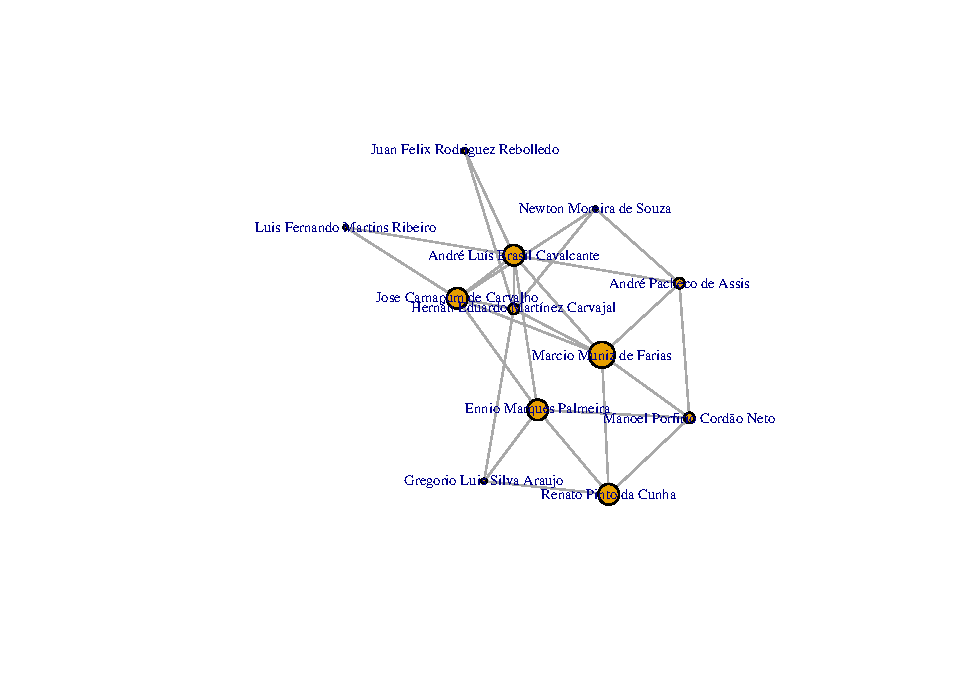
\includegraphics{LuanFreitas.relatorio2_files/figure-latex/unnamed-chunk-60-1.pdf}

\begin{Shaded}
\begin{Highlighting}[]
\NormalTok{reference_table <-}\StringTok{ }\NormalTok{graph}\OperatorTok{$}\NormalTok{nodes}
\KeywordTok{colnames}\NormalTok{(reference_table) <-}\StringTok{ }\KeywordTok{c}\NormalTok{(}
\StringTok{"IdLattes"}\NormalTok{,}
\StringTok{"Index"}\NormalTok{,}
\StringTok{"Docente"}\NormalTok{)}
\KeywordTok{kable}\NormalTok{(reference_table[,}\KeywordTok{c}\NormalTok{(}\DecValTok{2}\NormalTok{,}\DecValTok{1}\NormalTok{,}\DecValTok{3}\NormalTok{)], }\DataTypeTok{caption =} \StringTok{"Tabela de refer攼㹡ncia da an攼㸱lise de redes"}\NormalTok{)}
\end{Highlighting}
\end{Shaded}

\begin{longtable}[]{@{}lll@{}}
\caption{Tabela de referncia da anlise de redes}\tabularnewline
\toprule
Index & IdLattes & Docente\tabularnewline
\midrule
\endfirsthead
\toprule
Index & IdLattes & Docente\tabularnewline
\midrule
\endhead
1 & 1515779118499986 & André Luís Brasil Cavalcante\tabularnewline
2 & 2245433059787601 & Jose Camapum de Carvalho\tabularnewline
3 & 2409917419986324 & Hernán Eduardo Martínez Carvajal\tabularnewline
4 & 3468455656914958 & Ennio Marques Palmeira\tabularnewline
5 & 4739413536925106 & Luis Fernando Martins Ribeiro\tabularnewline
6 & 4778269687775430 & Manoel Porfirio Cordão Neto\tabularnewline
7 & 5345279954551868 & Marcio Muniz de Farias\tabularnewline
8 & 6075465233665208 & Gregorio Luis Silva Araujo\tabularnewline
9 & 8320758938514935 & Juan Felix Rodriguez Rebolledo\tabularnewline
10 & 8863234872460861 & Newton Moreira de Souza\tabularnewline
11 & 9013693430617718 & Renato Pinto da Cunha\tabularnewline
12 & 9477887320208504 & André Pacheco de Assis\tabularnewline
\bottomrule
\end{longtable}

O grafo ilustra o número de colaborações de cada autor pelo tamanho do
nó relacionado a seu índex da tabela de autores:

\begin{Shaded}
\begin{Highlighting}[]
\KeywordTok{plot}\NormalTok{(g,}
\DataTypeTok{vertex.size =} \KeywordTok{V}\NormalTok{(g)}\OperatorTok{$}\NormalTok{degree}\OperatorTok{*}\FloatTok{1.5}\NormalTok{,}
\DataTypeTok{vertex.label =}\NormalTok{ graph}\OperatorTok{$}\NormalTok{nodes}\OperatorTok{$}\NormalTok{label,}
\DataTypeTok{layout =} \KeywordTok{layout_nicely}\NormalTok{(g),}
\DataTypeTok{vertex.label.cex =} \FloatTok{0.6}\NormalTok{)}
\end{Highlighting}
\end{Shaded}

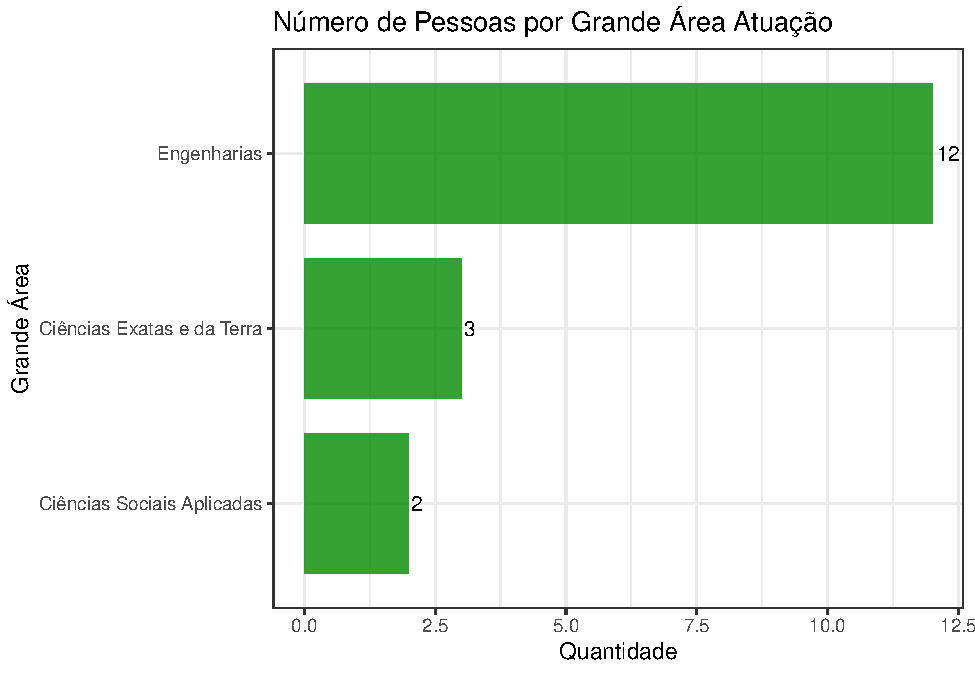
\includegraphics{LuanFreitas.relatorio2_files/figure-latex/unnamed-chunk-62-1.pdf}

O grafo ilustra o número de publicações de cada autor pelo tamanho do nó
relacionado a seu índex da tabela de autores:

\begin{Shaded}
\begin{Highlighting}[]
\KeywordTok{plot}\NormalTok{(g,}
\DataTypeTok{vertex.size =} \KeywordTok{na.omit}\NormalTok{(}\KeywordTok{round}\NormalTok{(}\KeywordTok{V}\NormalTok{(g)}\OperatorTok{$}\NormalTok{publicacao}\OperatorTok{/}\DecValTok{7}\NormalTok{)}\OperatorTok{*}\DecValTok{3}\NormalTok{),}
\DataTypeTok{vertex.label =}\NormalTok{ graph}\OperatorTok{$}\NormalTok{nodes}\OperatorTok{$}\NormalTok{label,}
\DataTypeTok{layout =} \KeywordTok{layout_nicely}\NormalTok{(g),}
\DataTypeTok{vertex.label.cex =} \FloatTok{0.6}\NormalTok{)}
\end{Highlighting}
\end{Shaded}

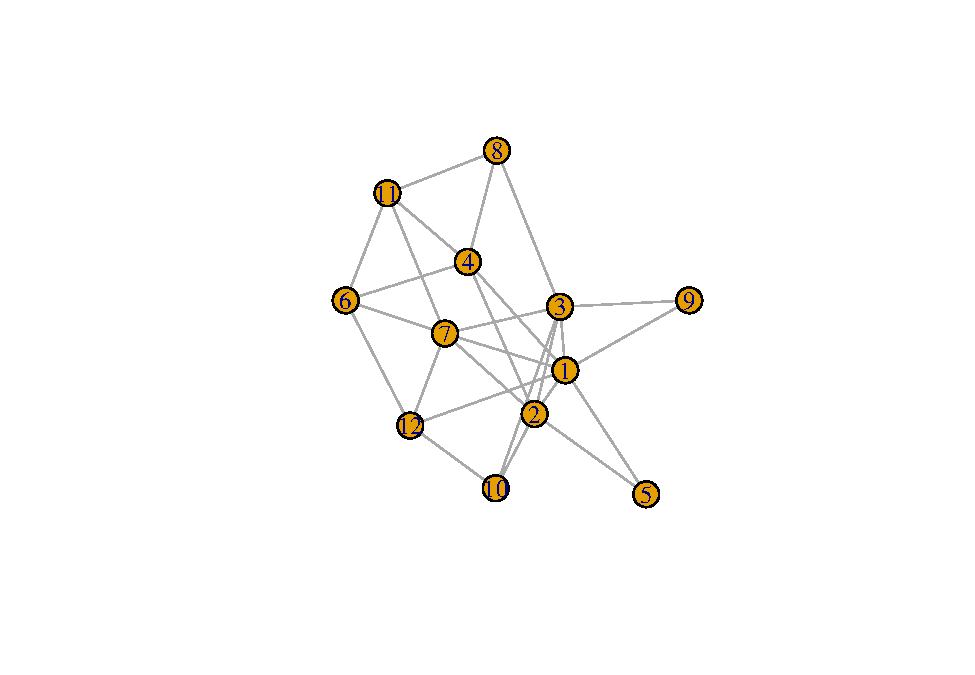
\includegraphics{LuanFreitas.relatorio2_files/figure-latex/unnamed-chunk-63-1.pdf}

O grafo 5 ilustra as comunidades entre os autores com agrupamentos no
grafo por cores:

\begin{Shaded}
\begin{Highlighting}[]
\NormalTok{kc =}\StringTok{ }\KeywordTok{fastgreedy.community}\NormalTok{(g)}
\KeywordTok{plot}\NormalTok{(kc, g, }\DataTypeTok{vertex.label =}\NormalTok{ graph}\OperatorTok{$}\NormalTok{nodes}\OperatorTok{$}\NormalTok{label, }\DataTypeTok{layout =} \KeywordTok{layout_nicely}\NormalTok{(g))}
\end{Highlighting}
\end{Shaded}

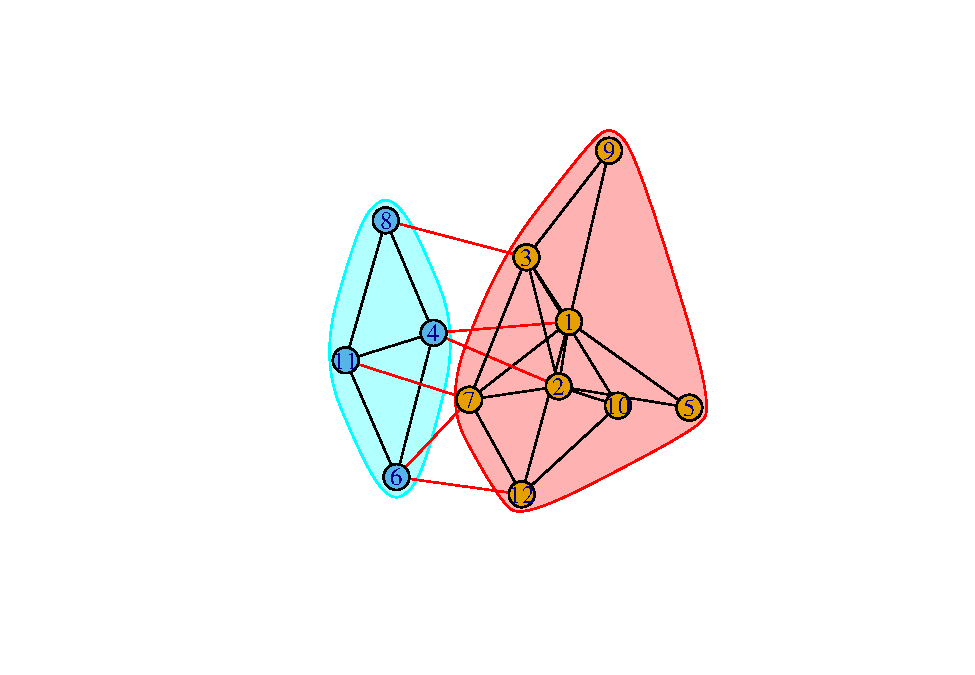
\includegraphics{LuanFreitas.relatorio2_files/figure-latex/unnamed-chunk-64-1.pdf}

\hypertarget{fase-5---avaliauxe7uxe3o}{%
\section{Fase 5 - Avaliação}\label{fase-5---avaliauxe7uxe3o}}

A fase de avaliação consiste na verificação de questões em relação aos
datasets que ainda não foram abordadas o suficiente. Dessa forma,
consiste em uma análise mais ``profunda'', por assim dizer, dos dados em
questão. A avaliação foi realizada de forma gráfica, sendo apresentados
a seguir: \#\# Avaliação dos resultados

\hypertarget{arquivo-perfil-1}{%
\subsubsection{Arquivo Perfil}\label{arquivo-perfil-1}}

O gráfico ilustra a quantidade de professores por grande área de
atuação:

\begin{Shaded}
\begin{Highlighting}[]
\NormalTok{profile }\OperatorTok
\StringTok{  }\KeywordTok{sapply}\NormalTok{(}\ControlFlowTok{function}\NormalTok{(x)}
    \KeywordTok{unique}\NormalTok{(x}\OperatorTok{$}\NormalTok{areas_de_atuacao}\OperatorTok{$}\NormalTok{grande_area)) }\OperatorTok
\StringTok{  }\KeywordTok{unlist}\NormalTok{() }\OperatorTok\StringTok{ }\KeywordTok{table}\NormalTok{() }\OperatorTok\StringTok{ }\KeywordTok{sort}\NormalTok{() }\OperatorTok\StringTok{ }\KeywordTok{as.data.frame}\NormalTok{() }\OperatorTok\StringTok{ }\KeywordTok{filter}\NormalTok{(}\OperatorTok{!}\NormalTok{. }\OperatorTok{==}\StringTok{ ""}\NormalTok{) }\OperatorTok
\StringTok{  }\KeywordTok{ggplot}\NormalTok{(}\KeywordTok{aes}\NormalTok{(}\DataTypeTok{x =}\NormalTok{ ., }\DataTypeTok{y =}\NormalTok{ Freq)) }\OperatorTok{+}\StringTok{ }\KeywordTok{geom_col}\NormalTok{(}\DataTypeTok{fill =} \StringTok{"green4"}\NormalTok{,}
                                          \DataTypeTok{alpha =} \FloatTok{0.8}\NormalTok{,}
                                          \DataTypeTok{width =} \FloatTok{0.8}\NormalTok{) }\OperatorTok{+}\StringTok{ }\KeywordTok{coord_flip}\NormalTok{() }\OperatorTok{+}\StringTok{ }\KeywordTok{geom_text}\NormalTok{(}\KeywordTok{aes}\NormalTok{(}\DataTypeTok{label =}\NormalTok{ Freq),}
                                                                                  \DataTypeTok{hjust =} \FloatTok{-0.2}\NormalTok{,}
                                                                                  \DataTypeTok{vjust =} \FloatTok{0.5}\NormalTok{,}
                                                                                  \DataTypeTok{size =} \FloatTok{3.5}\NormalTok{) }\OperatorTok{+}
\StringTok{  }\KeywordTok{labs}\NormalTok{(}\DataTypeTok{title =} \StringTok{"N昼㹡mero de Pessoas por Grande 挼㸱rea Atua攼㸷攼㸳o"}\NormalTok{, }\DataTypeTok{y =} \StringTok{"Quantidade"}\NormalTok{, }\DataTypeTok{x =}
         \StringTok{"Grande 挼㸱rea"}\NormalTok{) }\OperatorTok{+}\StringTok{ }\KeywordTok{theme_bw}\NormalTok{() }\OperatorTok{+}\StringTok{ }\KeywordTok{scale_y_continuous}\NormalTok{() }\OperatorTok{+}
\StringTok{  }\KeywordTok{scale_x_discrete}\NormalTok{(}
    \DataTypeTok{labels =} \KeywordTok{c}\NormalTok{(}
      \StringTok{'CIENCIAS_DA_SAUDE'}\NormalTok{ =}\StringTok{ 'Ci攼㹡ncias da Sa昼㹡de'}\NormalTok{,}
      \StringTok{'CIENCIAS_BIOLOGICAS'}\NormalTok{ =}\StringTok{ 'Ci攼㹡ncias Biol昼㸳gicas'}\NormalTok{,}
      \StringTok{'CIENCIAS_HUMANAS'}\NormalTok{ =}\StringTok{ 'Ci攼㹡ncias Humanas'}\NormalTok{,}
      \StringTok{"CIENCIAS_EXATAS_E_DA_TERRA"}\NormalTok{ =}\StringTok{ "Ci攼㹡ncias Exatas e da Terra"}\NormalTok{,}
      \StringTok{"CIENCIAS_SOCIAIS_APLICADAS"}\NormalTok{ =}\StringTok{ "Ci攼㹡ncias Sociais Aplicadas"}\NormalTok{,}
      \StringTok{"CIENCIAS_AGRARIAS"}\NormalTok{ =}\StringTok{ "Ci攼㹡ncias Agr攼㸱rias"}\NormalTok{,}
      \StringTok{"OUTROS"}\NormalTok{ =}\StringTok{ "Outros"}\NormalTok{,}
      \StringTok{"ENGENHARIAS"}\NormalTok{ =}\StringTok{ "Engenharias"}\NormalTok{,}
      \StringTok{"LINGUISTICA_LETRAS_E_ARTES"}\NormalTok{ =}\StringTok{ "Lingu攼㹤stica, Letras e Artes"}
\NormalTok{    )}
\NormalTok{  )}
\end{Highlighting}
\end{Shaded}

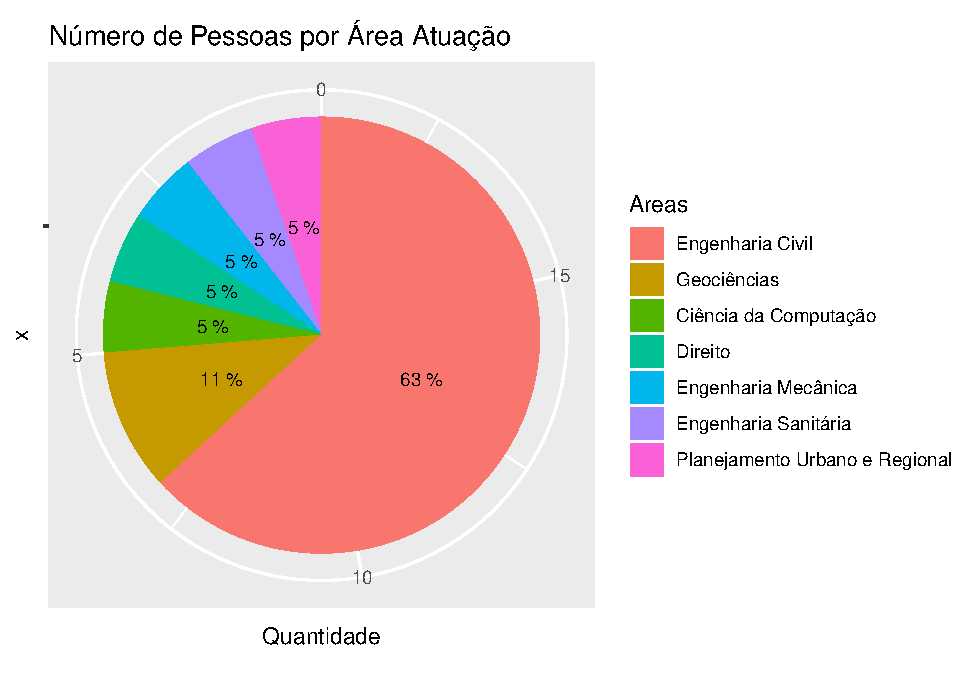
\includegraphics{LuanFreitas.relatorio2_files/figure-latex/unnamed-chunk-65-1.pdf}

O gráfico ilustra a quantidade de professores por grande área de atuação
(em forma de colunas):

\begin{Shaded}
\begin{Highlighting}[]
\NormalTok{profile }\OperatorTok
\StringTok{  }\KeywordTok{sapply}\NormalTok{(}\ControlFlowTok{function}\NormalTok{(x)}
    \KeywordTok{unique}\NormalTok{(x}\OperatorTok{$}\NormalTok{areas_de_atuacao}\OperatorTok{$}\NormalTok{area)) }\OperatorTok
\StringTok{  }\KeywordTok{unlist}\NormalTok{() }\OperatorTok\StringTok{ }\KeywordTok{table}\NormalTok{() }\OperatorTok\StringTok{ }\KeywordTok{sort}\NormalTok{() }\OperatorTok\StringTok{ }\KeywordTok{as.data.frame}\NormalTok{() }\OperatorTok\StringTok{ }\KeywordTok{filter}\NormalTok{(}\OperatorTok{!}\NormalTok{. }\OperatorTok{==}\StringTok{ ""}\NormalTok{) }\OperatorTok\StringTok{ }\KeywordTok{tail}\NormalTok{(}\DecValTok{20}\NormalTok{) }\OperatorTok
\StringTok{  }\KeywordTok{ggplot}\NormalTok{(}\KeywordTok{aes}\NormalTok{(}\DataTypeTok{x =}\NormalTok{ ., }\DataTypeTok{y =}\NormalTok{ Freq)) }\OperatorTok{+}\StringTok{ }\KeywordTok{geom_col}\NormalTok{(}\DataTypeTok{fill =} \StringTok{"green4"}\NormalTok{,}
                                          \DataTypeTok{alpha =} \FloatTok{0.8}\NormalTok{,}
                                          \DataTypeTok{width =} \FloatTok{0.8}\NormalTok{) }\OperatorTok{+}\StringTok{ }\KeywordTok{coord_flip}\NormalTok{() }\OperatorTok{+}
\StringTok{  }\KeywordTok{labs}\NormalTok{(}\DataTypeTok{title =} \StringTok{"N昼㹡mero de Pessoas por 挼㸱rea Atua攼㸷攼㸳o"}\NormalTok{, }\DataTypeTok{x =} \StringTok{"挼㸱rea de atua攼㸷攼㸳o"}\NormalTok{, }\DataTypeTok{y =}
         \StringTok{"Quantidade"}\NormalTok{) }\OperatorTok{+}
\StringTok{  }\KeywordTok{geom_text}\NormalTok{(}\KeywordTok{aes}\NormalTok{(}\DataTypeTok{label =}\NormalTok{ Freq),}
            \DataTypeTok{hjust =} \FloatTok{-0.2}\NormalTok{,}
            \DataTypeTok{vjust =} \FloatTok{0.3}\NormalTok{,}
            \DataTypeTok{size =} \FloatTok{3.5}\NormalTok{) }\OperatorTok{+}
\StringTok{  }\KeywordTok{scale_y_continuous}\NormalTok{(}\DataTypeTok{limits =} \KeywordTok{c}\NormalTok{(}\DecValTok{0}\NormalTok{, }\DecValTok{800}\NormalTok{)) }\OperatorTok{+}\StringTok{ }\KeywordTok{theme_bw}\NormalTok{()}
\end{Highlighting}
\end{Shaded}

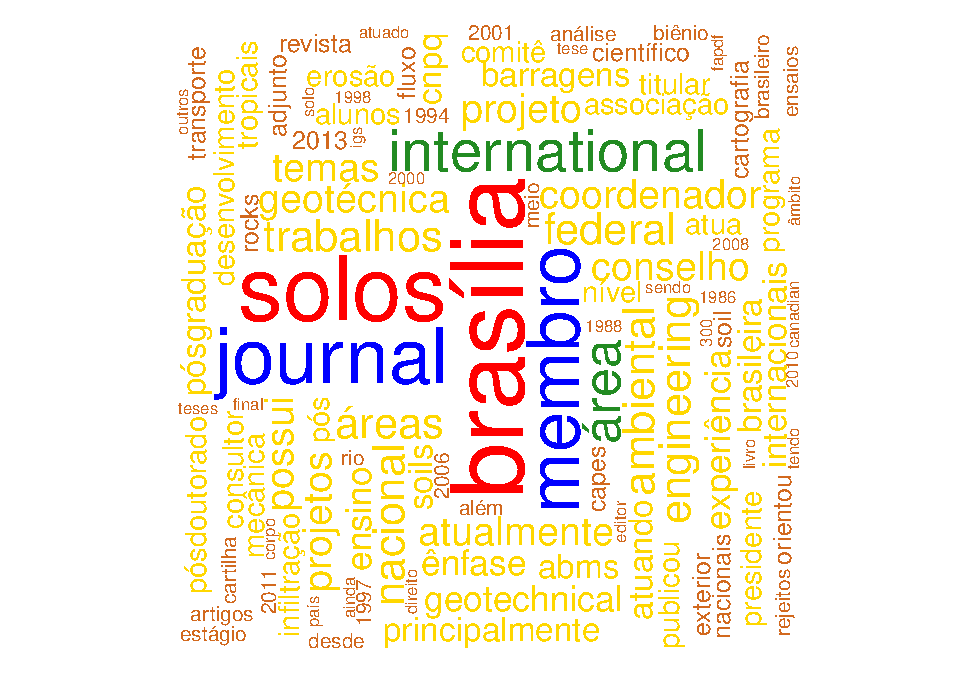
\includegraphics{LuanFreitas.relatorio2_files/figure-latex/unnamed-chunk-66-1.pdf}

O gráfico ilustra a quantidade de professores por grande área de atuação
(em forma de pizza):

\begin{Shaded}
\begin{Highlighting}[]
\KeywordTok{ggplot}\NormalTok{(areas_atuacao, }\KeywordTok{aes}\NormalTok{(}\DataTypeTok{x =} \StringTok{""}\NormalTok{, }\DataTypeTok{y =}\NormalTok{ Quantidade, }\DataTypeTok{fill =}\NormalTok{ Areas)) }\OperatorTok{+}
\StringTok{  }\KeywordTok{geom_bar}\NormalTok{(}\DataTypeTok{width =} \DecValTok{1}\NormalTok{, }\DataTypeTok{stat =} \StringTok{"identity"}\NormalTok{) }\OperatorTok{+}
\StringTok{  }\KeywordTok{coord_polar}\NormalTok{(}\StringTok{"y"}\NormalTok{, }\DataTypeTok{start =} \DecValTok{0}\NormalTok{, }\DataTypeTok{direction =} \DecValTok{-1}\NormalTok{) }\OperatorTok{+}
\StringTok{  }\KeywordTok{labs}\NormalTok{(}\DataTypeTok{title =} \StringTok{"N昼㹡mero de Pessoas por 挼㸱rea Atua攼㸷攼㸳o"}\NormalTok{) }\OperatorTok{+}
\StringTok{  }\KeywordTok{geom_text}\NormalTok{(}
    \DataTypeTok{data =}\NormalTok{ areas_atuacao,}
    \KeywordTok{aes}\NormalTok{(}
      \DataTypeTok{x =} \StringTok{""}\NormalTok{,}
      \DataTypeTok{y =}\NormalTok{ Quantidade,}
      \DataTypeTok{label =} \KeywordTok{paste}\NormalTok{(Porcentagem, }\StringTok{"%"}\NormalTok{)}
\NormalTok{    ),}
    \DataTypeTok{position =} \KeywordTok{position_stack}\NormalTok{(}\DataTypeTok{vjust =} \FloatTok{0.5}\NormalTok{),}
    \DataTypeTok{size =} \DecValTok{3}
\NormalTok{  )}
\end{Highlighting}
\end{Shaded}

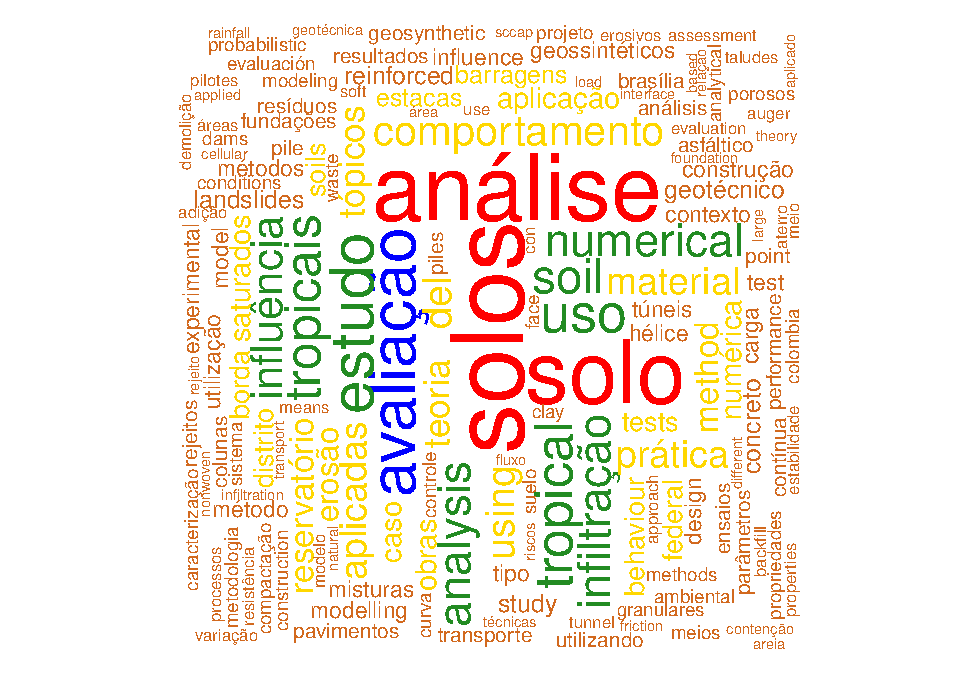
\includegraphics{LuanFreitas.relatorio2_files/figure-latex/unnamed-chunk-67-1.pdf}

O gráfico ilustra a quantidade de professores por grande área de atuação
(em forma de colunas):

\begin{Shaded}
\begin{Highlighting}[]
\NormalTok{profile }\OperatorTok
\StringTok{  }\KeywordTok{sapply}\NormalTok{(}\ControlFlowTok{function}\NormalTok{(x)}
    \KeywordTok{unique}\NormalTok{(x}\OperatorTok{$}\NormalTok{areas_de_atuacao}\OperatorTok{$}\NormalTok{sub_area)) }\OperatorTok
\StringTok{  }\KeywordTok{unlist}\NormalTok{() }\OperatorTok\StringTok{ }\KeywordTok{table}\NormalTok{() }\OperatorTok\StringTok{ }\KeywordTok{sort}\NormalTok{() }\OperatorTok\StringTok{ }\KeywordTok{as.data.frame}\NormalTok{() }\OperatorTok\StringTok{ }\KeywordTok{filter}\NormalTok{(}\OperatorTok{!}\NormalTok{. }\OperatorTok{==}\StringTok{ ""}\NormalTok{) }\OperatorTok\StringTok{ }\KeywordTok{tail}\NormalTok{(}\DecValTok{30}\NormalTok{) }\OperatorTok
\StringTok{  }\KeywordTok{ggplot}\NormalTok{(}\KeywordTok{aes}\NormalTok{(}\DataTypeTok{x =}\NormalTok{ ., }\DataTypeTok{y =}\NormalTok{ Freq)) }\OperatorTok{+}\StringTok{ }\KeywordTok{geom_col}\NormalTok{(}\DataTypeTok{fill =} \StringTok{"green4"}\NormalTok{,}
                                          \DataTypeTok{alpha =} \FloatTok{0.8}\NormalTok{,}
                                          \DataTypeTok{width =} \FloatTok{0.8}\NormalTok{) }\OperatorTok{+}\StringTok{ }\KeywordTok{coord_flip}\NormalTok{() }\OperatorTok{+}
\StringTok{  }\KeywordTok{geom_text}\NormalTok{(}\KeywordTok{aes}\NormalTok{(}\DataTypeTok{label =}\NormalTok{ Freq),}
            \DataTypeTok{hjust =} \FloatTok{-0.2}\NormalTok{,}
            \DataTypeTok{vjust =} \FloatTok{0.3}\NormalTok{,}
            \DataTypeTok{size =} \FloatTok{3.5}\NormalTok{) }\OperatorTok{+}
\StringTok{  }\KeywordTok{labs}\NormalTok{(}\DataTypeTok{title =} \StringTok{"N昼㹡mero de Pessoas por Sub 挼㸱rea atua攼㸷攼㸳o"}\NormalTok{, }\DataTypeTok{x =} \StringTok{"Sub 挼㸱rea"}\NormalTok{, }\DataTypeTok{y =}
         \StringTok{"Quantidade"}\NormalTok{) }\OperatorTok{+}
\StringTok{  }\KeywordTok{scale_y_continuous}\NormalTok{(}\DataTypeTok{limits =} \KeywordTok{c}\NormalTok{(}\DecValTok{0}\NormalTok{, }\DecValTok{300}\NormalTok{)) }\OperatorTok{+}\StringTok{ }\KeywordTok{theme_bw}\NormalTok{()}
\end{Highlighting}
\end{Shaded}

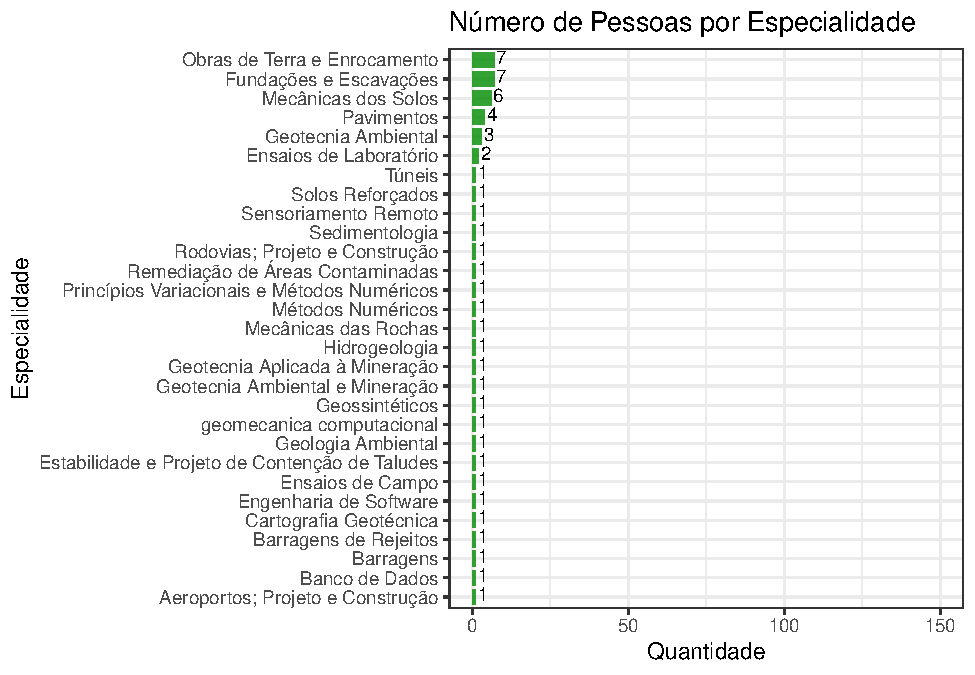
\includegraphics{LuanFreitas.relatorio2_files/figure-latex/unnamed-chunk-68-1.pdf}

O gráfico ilustra a quantidade de professores por grande área de atuação
(em forma de pizza):

\begin{Shaded}
\begin{Highlighting}[]
\KeywordTok{ggplot}\NormalTok{(subarea, }\KeywordTok{aes}\NormalTok{(}\DataTypeTok{x =} \StringTok{""}\NormalTok{, }\DataTypeTok{y =}\NormalTok{ Quantidade, }\DataTypeTok{fill =}\NormalTok{ Subarea)) }\OperatorTok{+}
\StringTok{  }\KeywordTok{geom_bar}\NormalTok{(}\DataTypeTok{width =} \DecValTok{1}\NormalTok{, }\DataTypeTok{stat =} \StringTok{"identity"}\NormalTok{) }\OperatorTok{+}
\StringTok{  }\KeywordTok{coord_polar}\NormalTok{(}\StringTok{"y"}\NormalTok{, }\DataTypeTok{start =} \DecValTok{0}\NormalTok{, }\DataTypeTok{direction =} \DecValTok{-1}\NormalTok{) }\OperatorTok{+}
\StringTok{  }\KeywordTok{labs}\NormalTok{(}\DataTypeTok{title =} \StringTok{"N昼㹡mero de Pessoas por Sub 挼㸱rea atua攼㸷攼㸳o"}\NormalTok{) }\OperatorTok{+}
\StringTok{  }\KeywordTok{geom_text}\NormalTok{(}
    \DataTypeTok{data =}\NormalTok{ subarea,}
    \KeywordTok{aes}\NormalTok{(}
      \DataTypeTok{x =} \StringTok{""}\NormalTok{,}
      \DataTypeTok{y =}\NormalTok{ Quantidade,}
      \DataTypeTok{label =} \KeywordTok{paste}\NormalTok{(Porcentagem, }\StringTok{"%"}\NormalTok{)}
\NormalTok{    ),}
    \DataTypeTok{position =} \KeywordTok{position_stack}\NormalTok{(}\DataTypeTok{vjust =} \FloatTok{0.5}\NormalTok{),}
    \DataTypeTok{size =} \DecValTok{3}
\NormalTok{  )}
\end{Highlighting}
\end{Shaded}

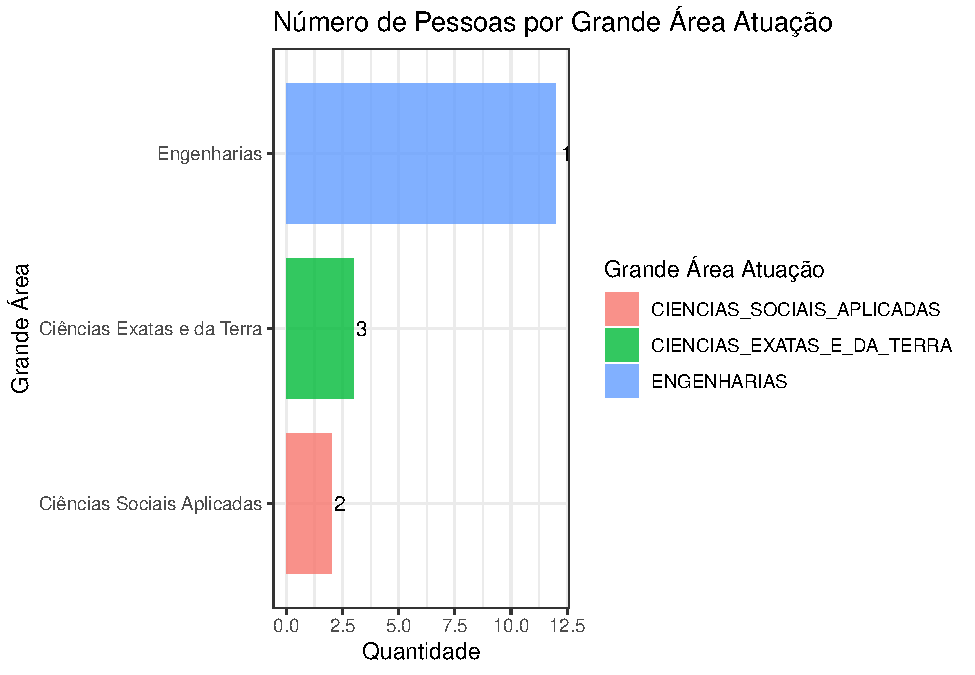
\includegraphics{LuanFreitas.relatorio2_files/figure-latex/unnamed-chunk-69-1.pdf}

O gráfico ilustra a quantidade de professores por especialidade (em
forma de colunas):

\begin{Shaded}
\begin{Highlighting}[]
\NormalTok{profile }\OperatorTok
\StringTok{  }\KeywordTok{sapply}\NormalTok{(}\ControlFlowTok{function}\NormalTok{(x)}
    \KeywordTok{unique}\NormalTok{(x}\OperatorTok{$}\NormalTok{areas_de_atuacao}\OperatorTok{$}\NormalTok{especialidade)) }\OperatorTok
\StringTok{  }\KeywordTok{unlist}\NormalTok{() }\OperatorTok\StringTok{ }\KeywordTok{table}\NormalTok{() }\OperatorTok\StringTok{ }\KeywordTok{sort}\NormalTok{() }\OperatorTok\StringTok{ }\KeywordTok{as.data.frame}\NormalTok{() }\OperatorTok\StringTok{ }\KeywordTok{filter}\NormalTok{(}\OperatorTok{!}\NormalTok{. }\OperatorTok{==}\StringTok{ ""}\NormalTok{) }\OperatorTok\StringTok{ }\KeywordTok{tail}\NormalTok{(}\DecValTok{29}\NormalTok{) }\OperatorTok
\StringTok{  }\KeywordTok{ggplot}\NormalTok{(}\KeywordTok{aes}\NormalTok{(}\DataTypeTok{x =}\NormalTok{ ., }\DataTypeTok{y =}\NormalTok{ Freq)) }\OperatorTok{+}\StringTok{ }\KeywordTok{geom_col}\NormalTok{(}\DataTypeTok{fill =} \StringTok{"green4"}\NormalTok{,}
                                          \DataTypeTok{alpha =} \FloatTok{0.8}\NormalTok{,}
                                          \DataTypeTok{width =} \FloatTok{0.8}\NormalTok{) }\OperatorTok{+}\StringTok{ }\KeywordTok{coord_flip}\NormalTok{() }\OperatorTok{+}
\StringTok{  }\KeywordTok{labs}\NormalTok{(}\DataTypeTok{title =} \StringTok{"N昼㹡mero de Pessoas por Especialidade"}\NormalTok{, }\DataTypeTok{x =} \StringTok{"Especialidade"}\NormalTok{, }\DataTypeTok{y =}
         \StringTok{"Quantidade"}\NormalTok{) }\OperatorTok{+}
\StringTok{  }\KeywordTok{geom_text}\NormalTok{(}\KeywordTok{aes}\NormalTok{(}\DataTypeTok{label =}\NormalTok{ Freq),}
            \DataTypeTok{hjust =} \FloatTok{-0.2}\NormalTok{,}
            \DataTypeTok{vjust =} \FloatTok{0.3}\NormalTok{,}
            \DataTypeTok{size =} \FloatTok{3.0}\NormalTok{) }\OperatorTok{+}
\StringTok{  }\KeywordTok{theme_bw}\NormalTok{() }\OperatorTok{+}
\StringTok{  }\KeywordTok{scale_y_continuous}\NormalTok{(}\DataTypeTok{limits =} \KeywordTok{c}\NormalTok{(}\DecValTok{0}\NormalTok{, }\DecValTok{150}\NormalTok{))}
\end{Highlighting}
\end{Shaded}

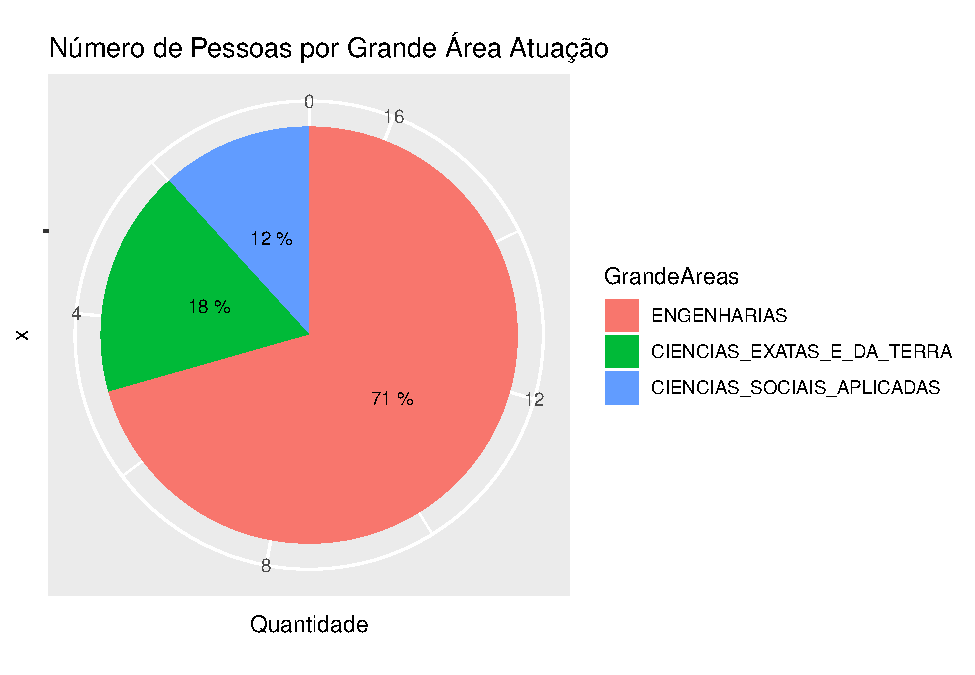
\includegraphics{LuanFreitas.relatorio2_files/figure-latex/unnamed-chunk-70-1.pdf}

O gráfico ilustra a quantidade de professores por especialidade (em
forma de barras):

\begin{Shaded}
\begin{Highlighting}[]
\KeywordTok{ggplot}\NormalTok{(especialidades_frequentes,}
       \KeywordTok{aes}\NormalTok{(}\DataTypeTok{x =} \StringTok{""}\NormalTok{, }\DataTypeTok{y =}\NormalTok{ Quantidade, }\DataTypeTok{fill =}\NormalTok{ Especialidade)) }\OperatorTok{+}
\StringTok{  }\KeywordTok{labs}\NormalTok{(}\DataTypeTok{title =} \StringTok{"N昼㹡mero de Pessoas por Especialidade"}\NormalTok{) }\OperatorTok{+}
\StringTok{  }\KeywordTok{geom_bar}\NormalTok{(}\DataTypeTok{width =} \DecValTok{1}\NormalTok{, }\DataTypeTok{stat =} \StringTok{"identity"}\NormalTok{) }\OperatorTok{+}
\StringTok{  }\KeywordTok{geom_text}\NormalTok{(}
    \DataTypeTok{data =}\NormalTok{ especialidades_frequentes,}
    \KeywordTok{aes}\NormalTok{(}\DataTypeTok{x =} \StringTok{""}\NormalTok{, }\DataTypeTok{y =}\NormalTok{ Quantidade, }\DataTypeTok{label =}\NormalTok{ Quantidade),}
    \DataTypeTok{position =} \KeywordTok{position_stack}\NormalTok{(}\DataTypeTok{vjust =} \FloatTok{0.5}\NormalTok{),}
    \DataTypeTok{size =} \DecValTok{3}
\NormalTok{  )}
\end{Highlighting}
\end{Shaded}

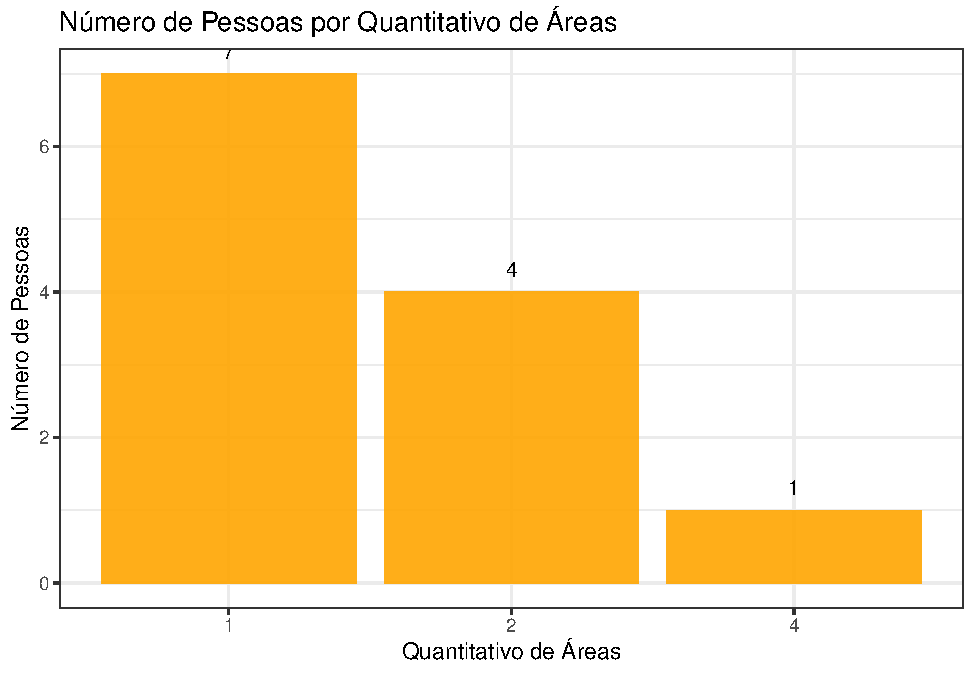
\includegraphics{LuanFreitas.relatorio2_files/figure-latex/unnamed-chunk-71-1.pdf}

O gráfico ilustra a quantidade de professores por quantitativo de grande
áreas:

\begin{Shaded}
\begin{Highlighting}[]
\NormalTok{profile }\OperatorTok
\StringTok{  }\KeywordTok{sapply}\NormalTok{(}\ControlFlowTok{function}\NormalTok{(x)}
    \KeywordTok{length}\NormalTok{(}\KeywordTok{unique}\NormalTok{(x}\OperatorTok{$}\NormalTok{areas_de_atuacao}\OperatorTok{$}\NormalTok{grande_area))) }\OperatorTok
\StringTok{  }\KeywordTok{unlist}\NormalTok{() }\OperatorTok\StringTok{ }\KeywordTok{table}\NormalTok{() }\OperatorTok\StringTok{ }\KeywordTok{sort}\NormalTok{() }\OperatorTok\StringTok{ }\KeywordTok{rev}\NormalTok{() }\OperatorTok\StringTok{ }\KeywordTok{as.data.frame}\NormalTok{() }\OperatorTok
\StringTok{  }\KeywordTok{ggplot}\NormalTok{(}\KeywordTok{aes}\NormalTok{(}\DataTypeTok{x =}\NormalTok{ ., }\DataTypeTok{y =}\NormalTok{ Freq)) }\OperatorTok{+}\StringTok{ }\KeywordTok{geom_col}\NormalTok{(}\DataTypeTok{fill =} \StringTok{"orange"}\NormalTok{, }\DataTypeTok{alpha =} \FloatTok{0.9}\NormalTok{) }\OperatorTok{+}
\StringTok{  }\KeywordTok{geom_text}\NormalTok{(}\KeywordTok{aes}\NormalTok{(}\DataTypeTok{label =}\NormalTok{ Freq), }\DataTypeTok{size =} \FloatTok{3.5}\NormalTok{, }\DataTypeTok{vjust =} \DecValTok{-1}\NormalTok{) }\OperatorTok{+}
\StringTok{  }\KeywordTok{labs}\NormalTok{(}\DataTypeTok{title =} \StringTok{"N昼㹡mero de Pessoas por Quantitativo de Grande 挼㸱reas"}\NormalTok{,}
       \DataTypeTok{y =} \StringTok{"N昼㹡mero de Pessoas"}\NormalTok{, }\DataTypeTok{x =} \StringTok{"Quantitativo de Grande 挼㸱reas"}\NormalTok{) }\OperatorTok{+}\StringTok{ }\KeywordTok{theme_bw}\NormalTok{()}
\end{Highlighting}
\end{Shaded}

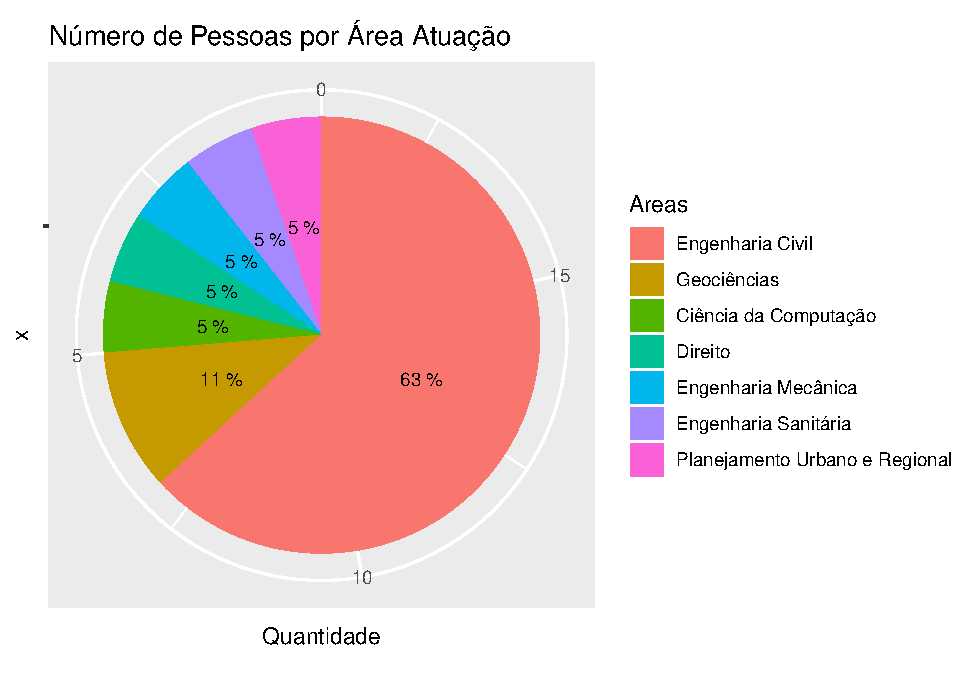
\includegraphics{LuanFreitas.relatorio2_files/figure-latex/unnamed-chunk-72-1.pdf}

O gráfico ilustra a quantidade de professores por quantitativo de áreas:

\begin{Shaded}
\begin{Highlighting}[]
\NormalTok{profile }\OperatorTok
\StringTok{  }\KeywordTok{sapply}\NormalTok{(}\ControlFlowTok{function}\NormalTok{(x)}
    \KeywordTok{length}\NormalTok{(}\KeywordTok{unique}\NormalTok{(x}\OperatorTok{$}\NormalTok{areas_de_atuacao}\OperatorTok{$}\NormalTok{area))) }\OperatorTok
\StringTok{  }\KeywordTok{unlist}\NormalTok{() }\OperatorTok\StringTok{ }\KeywordTok{table}\NormalTok{() }\OperatorTok\StringTok{ }\KeywordTok{sort}\NormalTok{() }\OperatorTok\StringTok{ }\KeywordTok{rev}\NormalTok{() }\OperatorTok\StringTok{ }\KeywordTok{as.data.frame}\NormalTok{() }\OperatorTok
\StringTok{  }\KeywordTok{ggplot}\NormalTok{(}\KeywordTok{aes}\NormalTok{(}\DataTypeTok{x =}\NormalTok{ ., }\DataTypeTok{y =}\NormalTok{ Freq)) }\OperatorTok{+}\StringTok{ }\KeywordTok{geom_col}\NormalTok{(}\DataTypeTok{fill =} \StringTok{"orange"}\NormalTok{, }\DataTypeTok{alpha =} \FloatTok{0.9}\NormalTok{) }\OperatorTok{+}
\StringTok{  }\KeywordTok{geom_text}\NormalTok{(}\KeywordTok{aes}\NormalTok{(}\DataTypeTok{label =}\NormalTok{ Freq), }\DataTypeTok{size =} \FloatTok{3.5}\NormalTok{, }\DataTypeTok{vjust =} \DecValTok{-1}\NormalTok{) }\OperatorTok{+}
\StringTok{  }\KeywordTok{labs}\NormalTok{(}\DataTypeTok{title =} \StringTok{"N昼㹡mero de Pessoas por Quantitativo de 挼㸱reas"}\NormalTok{,}
       \DataTypeTok{y =} \StringTok{"N昼㹡mero de Pessoas"}\NormalTok{, }\DataTypeTok{x =} \StringTok{"Quantitativo de 挼㸱reas"}\NormalTok{) }\OperatorTok{+}\StringTok{ }\KeywordTok{theme_bw}\NormalTok{()}
\end{Highlighting}
\end{Shaded}

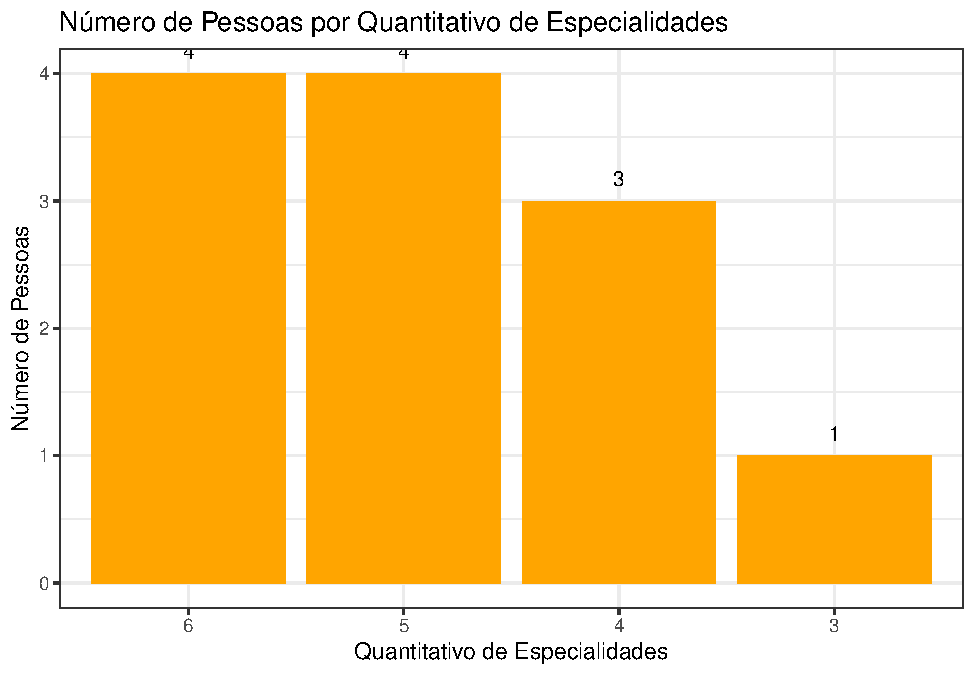
\includegraphics{LuanFreitas.relatorio2_files/figure-latex/unnamed-chunk-73-1.pdf}

O gráfico ilustra a quantidade de professores por quantitativo de
sub-áreas:

\begin{Shaded}
\begin{Highlighting}[]
\NormalTok{profile }\OperatorTok
\StringTok{  }\KeywordTok{sapply}\NormalTok{(}\ControlFlowTok{function}\NormalTok{(x)}
    \KeywordTok{length}\NormalTok{(}\KeywordTok{unique}\NormalTok{(x}\OperatorTok{$}\NormalTok{areas_de_atuacao}\OperatorTok{$}\NormalTok{sub_area))) }\OperatorTok
\StringTok{  }\KeywordTok{unlist}\NormalTok{() }\OperatorTok\StringTok{ }\KeywordTok{table}\NormalTok{() }\OperatorTok\StringTok{ }\KeywordTok{sort}\NormalTok{() }\OperatorTok\StringTok{ }\KeywordTok{rev}\NormalTok{() }\OperatorTok\StringTok{ }\KeywordTok{as.data.frame}\NormalTok{() }\OperatorTok
\StringTok{  }\KeywordTok{ggplot}\NormalTok{(}\KeywordTok{aes}\NormalTok{(}\DataTypeTok{x =}\NormalTok{ ., }\DataTypeTok{y =}\NormalTok{ Freq)) }\OperatorTok{+}\StringTok{ }\KeywordTok{geom_col}\NormalTok{(}\DataTypeTok{fill =} \StringTok{"orange"}\NormalTok{, }\DataTypeTok{alpha =} \FloatTok{0.9}\NormalTok{) }\OperatorTok{+}
\StringTok{  }\KeywordTok{geom_text}\NormalTok{(}\KeywordTok{aes}\NormalTok{(}\DataTypeTok{label =}\NormalTok{ Freq), }\DataTypeTok{size =} \FloatTok{3.5}\NormalTok{, }\DataTypeTok{vjust =} \DecValTok{-1}\NormalTok{) }\OperatorTok{+}
\StringTok{  }\KeywordTok{labs}\NormalTok{(}\DataTypeTok{title =} \StringTok{"N昼㹡mero de Pessoas por Quantitativo de Sub 挼㸱reas"}\NormalTok{,}
       \DataTypeTok{y =} \StringTok{"N昼㹡mero de Pessoas"}\NormalTok{, }\DataTypeTok{x =} \StringTok{"Quantitativo de Sub 挼㸱reas"}\NormalTok{) }\OperatorTok{+}\StringTok{ }\KeywordTok{theme_bw}\NormalTok{()}
\end{Highlighting}
\end{Shaded}

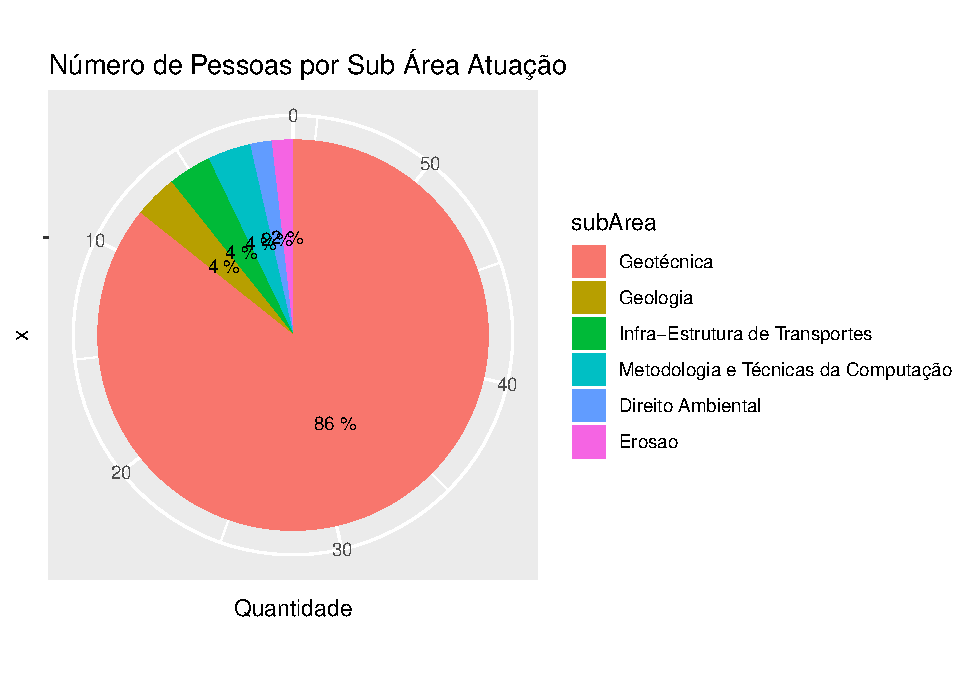
\includegraphics{LuanFreitas.relatorio2_files/figure-latex/unnamed-chunk-74-1.pdf}

O gráfico ilustra a quantidade de professores por quantitativo de
especialidades:

\begin{Shaded}
\begin{Highlighting}[]
\NormalTok{profile }\OperatorTok
\StringTok{  }\KeywordTok{sapply}\NormalTok{(}\ControlFlowTok{function}\NormalTok{(x)}
    \KeywordTok{length}\NormalTok{(}\KeywordTok{unique}\NormalTok{(x}\OperatorTok{$}\NormalTok{areas_de_atuacao}\OperatorTok{$}\NormalTok{especialidade))) }\OperatorTok
\StringTok{  }\KeywordTok{unlist}\NormalTok{() }\OperatorTok\StringTok{ }\KeywordTok{table}\NormalTok{() }\OperatorTok\StringTok{ }\KeywordTok{sort}\NormalTok{() }\OperatorTok\StringTok{ }\KeywordTok{rev}\NormalTok{() }\OperatorTok\StringTok{ }\KeywordTok{as.data.frame}\NormalTok{() }\OperatorTok
\StringTok{  }\KeywordTok{ggplot}\NormalTok{(}\KeywordTok{aes}\NormalTok{(}\DataTypeTok{x =}\NormalTok{ ., }\DataTypeTok{y =}\NormalTok{ Freq)) }\OperatorTok{+}\StringTok{ }\KeywordTok{geom_col}\NormalTok{(}\DataTypeTok{fill =} \StringTok{"orange"}\NormalTok{) }\OperatorTok{+}
\StringTok{  }\KeywordTok{geom_text}\NormalTok{(}\KeywordTok{aes}\NormalTok{(}\DataTypeTok{label =}\NormalTok{ Freq), }\DataTypeTok{size =} \FloatTok{3.5}\NormalTok{, }\DataTypeTok{vjust =} \DecValTok{-1}\NormalTok{) }\OperatorTok{+}
\StringTok{  }\KeywordTok{labs}\NormalTok{(}\DataTypeTok{title =} \StringTok{"N昼㹡mero de Pessoas por Quantitativo de Especialidades"}\NormalTok{,}
       \DataTypeTok{y =} \StringTok{"N昼㹡mero de Pessoas"}\NormalTok{, }\DataTypeTok{x =} \StringTok{"Quantitativo de Especialidades"}\NormalTok{) }\OperatorTok{+}\StringTok{ }\KeywordTok{theme_bw}\NormalTok{()}
\end{Highlighting}
\end{Shaded}

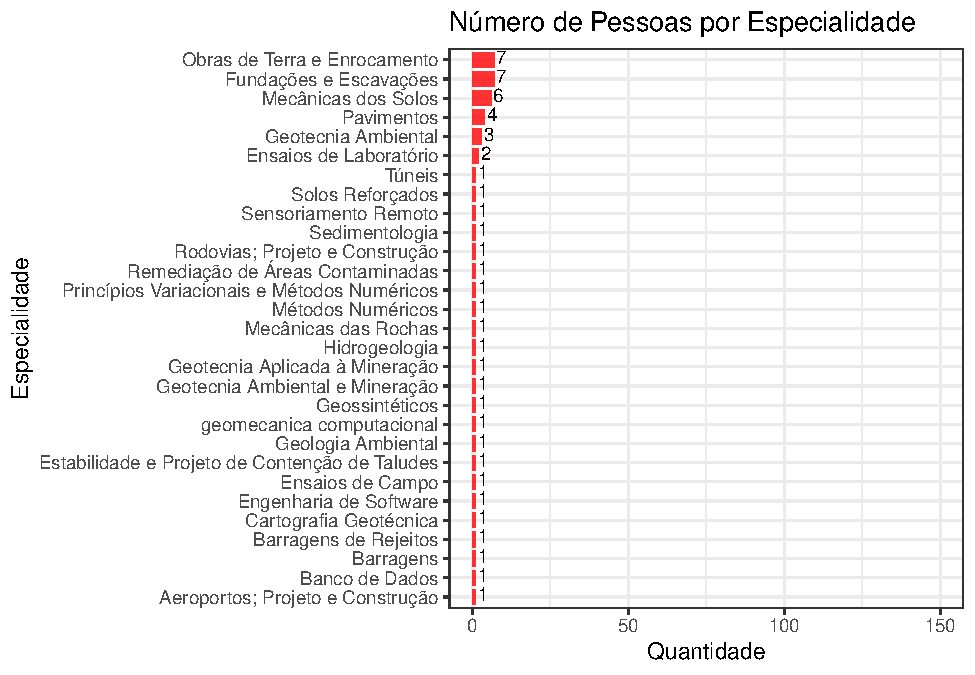
\includegraphics{LuanFreitas.relatorio2_files/figure-latex/unnamed-chunk-75-1.pdf}

O gráfico ilustra a quantidade de artigos publicados por quantitativo de
professores:

\begin{Shaded}
\begin{Highlighting}[]
\NormalTok{profile }\OperatorTok
\StringTok{  }\KeywordTok{sapply}\NormalTok{(}\ControlFlowTok{function}\NormalTok{(x)}
    \KeywordTok{length}\NormalTok{(x}\OperatorTok{$}\NormalTok{producao_bibiografica}\OperatorTok{$}\NormalTok{PERIODICO}\OperatorTok{$}\NormalTok{ano)) }\OperatorTok
\StringTok{  }\KeywordTok{unlist}\NormalTok{() }\OperatorTok\StringTok{ }\KeywordTok{table}\NormalTok{()   }\OperatorTok\StringTok{ }\KeywordTok{rev}\NormalTok{() }\OperatorTok\StringTok{ }\KeywordTok{as.data.frame}\NormalTok{() }\OperatorTok
\StringTok{  }\KeywordTok{ggplot}\NormalTok{(}\KeywordTok{aes}\NormalTok{(}\DataTypeTok{x =}\NormalTok{ ., }\DataTypeTok{y =}\NormalTok{ Freq)) }\OperatorTok{+}\StringTok{ }\KeywordTok{geom_col}\NormalTok{(}\DataTypeTok{fill =} \StringTok{"green4"}\NormalTok{, }\DataTypeTok{width =} \FloatTok{0.6}\NormalTok{) }\OperatorTok{+}
\StringTok{  }\KeywordTok{labs}\NormalTok{(}\DataTypeTok{title =} \StringTok{"N昼㹡mero de Artigos Publicados por Quantitativo de pessoas"}\NormalTok{, }\DataTypeTok{y =} \StringTok{"Pessoas"}\NormalTok{, }\DataTypeTok{x =} \StringTok{"Publica攼㸷昼㸵es"}\NormalTok{) }\OperatorTok{+}
\StringTok{  }\KeywordTok{theme_bw}\NormalTok{() }\OperatorTok{+}\StringTok{ }\KeywordTok{coord_flip}\NormalTok{()}
\end{Highlighting}
\end{Shaded}

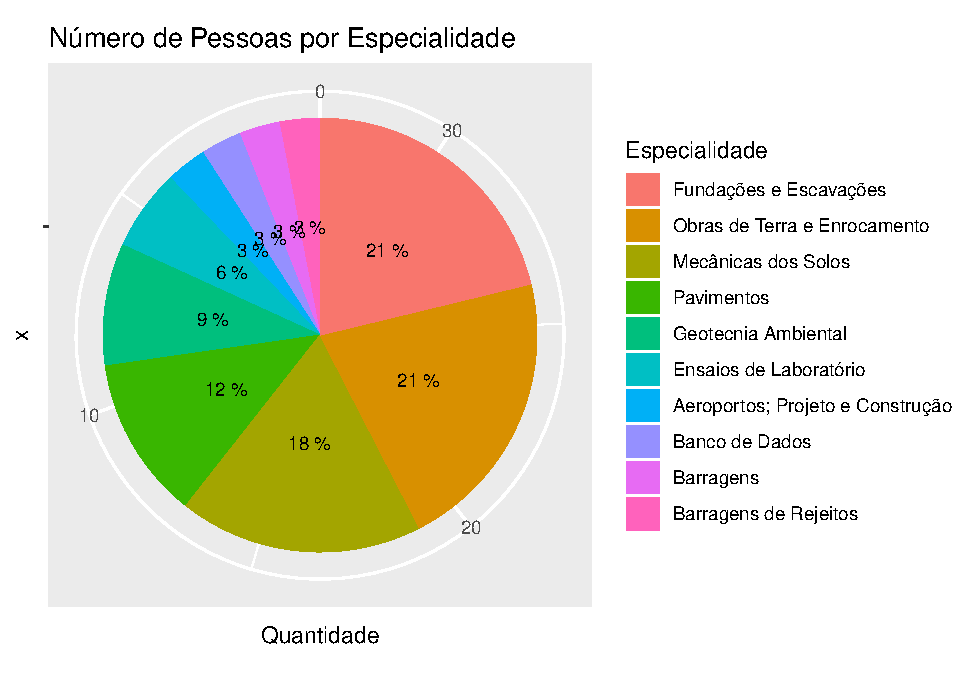
\includegraphics{LuanFreitas.relatorio2_files/figure-latex/unnamed-chunk-76-1.pdf}

O gráfico ilustra a quantidade de capítulo publicados por quantitativo
de professores:

\begin{Shaded}
\begin{Highlighting}[]
\NormalTok{profile }\OperatorTok
\StringTok{  }\KeywordTok{sapply}\NormalTok{(}\ControlFlowTok{function}\NormalTok{(x)}
    \KeywordTok{length}\NormalTok{(x}\OperatorTok{$}\NormalTok{producao_bibiografica}\OperatorTok{$}\NormalTok{CAPITULO_DE_LIVRO}\OperatorTok{$}\NormalTok{ano)) }\OperatorTok
\StringTok{  }\KeywordTok{unlist}\NormalTok{() }\OperatorTok\StringTok{ }\KeywordTok{table}\NormalTok{() }\OperatorTok\StringTok{ }\KeywordTok{rev}\NormalTok{() }\OperatorTok\StringTok{ }\KeywordTok{as.data.frame}\NormalTok{() }\OperatorTok
\StringTok{  }\KeywordTok{ggplot}\NormalTok{(}\KeywordTok{aes}\NormalTok{(}\DataTypeTok{x =}\NormalTok{ ., }\DataTypeTok{y =}\NormalTok{ Freq)) }\OperatorTok{+}\StringTok{ }\KeywordTok{geom_col}\NormalTok{(}\DataTypeTok{fill =} \StringTok{"green4"}\NormalTok{, }\DataTypeTok{width =} \FloatTok{0.8}\NormalTok{) }\OperatorTok{+}\StringTok{ }\KeywordTok{coord_flip}\NormalTok{() }\OperatorTok{+}
\StringTok{  }\KeywordTok{labs}\NormalTok{(}\DataTypeTok{title =} \StringTok{"N昼㹡mero de Cap攼㹤tulos de Livros por Quantitativo de pessoas"}\NormalTok{, }\DataTypeTok{y =} \StringTok{"Pessoas"}\NormalTok{, }\DataTypeTok{x =} \StringTok{"Publica攼㸷昼㸵es"}\NormalTok{) }\OperatorTok{+}
\StringTok{  }\KeywordTok{scale_x_discrete}\NormalTok{() }\OperatorTok{+}\StringTok{ }\KeywordTok{theme_bw}\NormalTok{() }\OperatorTok{+}\StringTok{ }\KeywordTok{geom_text}\NormalTok{(}\KeywordTok{aes}\NormalTok{(}\DataTypeTok{label =}\NormalTok{ Freq),}
                                              \DataTypeTok{hjust =} \FloatTok{-0.3}\NormalTok{,}
                                              \DataTypeTok{vjust =} \FloatTok{0.3}\NormalTok{,}
                                              \DataTypeTok{size =} \FloatTok{3.1}\NormalTok{) }\OperatorTok{+}\StringTok{ }\KeywordTok{scale_y_continuous}\NormalTok{(}\DataTypeTok{limits =} \KeywordTok{c}\NormalTok{(}\DecValTok{0}\NormalTok{, }\DecValTok{500}\NormalTok{))}
\end{Highlighting}
\end{Shaded}

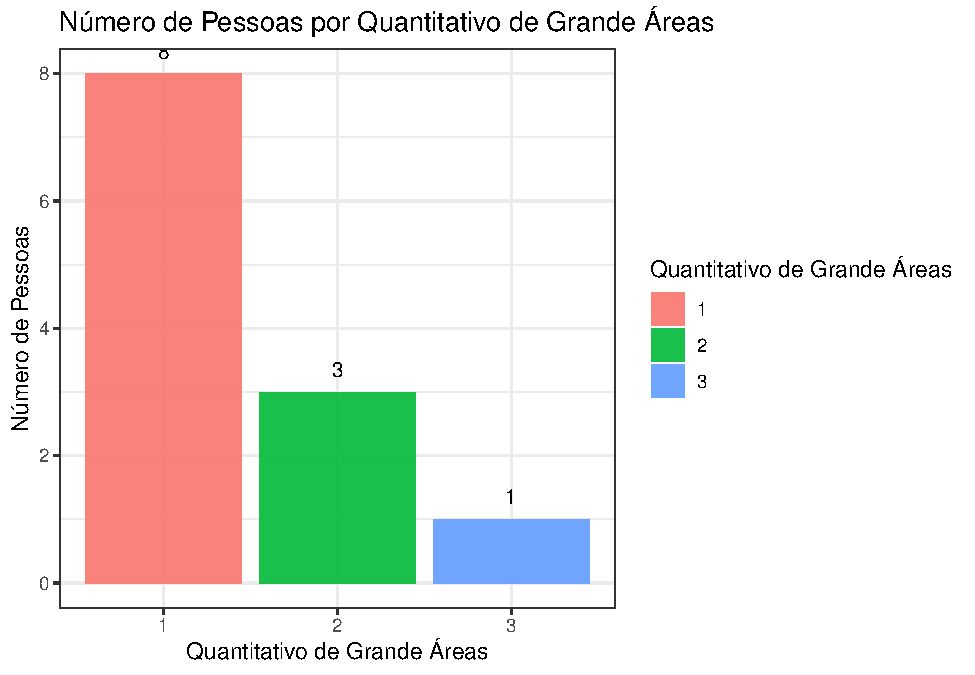
\includegraphics{LuanFreitas.relatorio2_files/figure-latex/unnamed-chunk-77-1.pdf}

O gráfico ilustra a quantidade de livros publicados por quantitativo de
professores:

\begin{Shaded}
\begin{Highlighting}[]
\NormalTok{profile }\OperatorTok
\StringTok{  }\KeywordTok{sapply}\NormalTok{(}\ControlFlowTok{function}\NormalTok{(x)}
    \KeywordTok{length}\NormalTok{(x}\OperatorTok{$}\NormalTok{producao_bibiografica}\OperatorTok{$}\NormalTok{LIVRO}\OperatorTok{$}\NormalTok{ano)) }\OperatorTok
\StringTok{  }\KeywordTok{unlist}\NormalTok{() }\OperatorTok\StringTok{ }\KeywordTok{table}\NormalTok{() }\OperatorTok\StringTok{ }\KeywordTok{rev}\NormalTok{() }\OperatorTok\StringTok{ }\KeywordTok{as.data.frame}\NormalTok{() }\OperatorTok
\StringTok{  }\KeywordTok{ggplot}\NormalTok{(}\KeywordTok{aes}\NormalTok{(}\DataTypeTok{x =}\NormalTok{ ., }\DataTypeTok{y =}\NormalTok{ Freq)) }\OperatorTok{+}\StringTok{ }\KeywordTok{geom_col}\NormalTok{(}\DataTypeTok{fill =} \StringTok{"green4"}\NormalTok{, }\DataTypeTok{width =} \FloatTok{0.5}\NormalTok{) }\OperatorTok{+}\StringTok{ }\KeywordTok{coord_flip}\NormalTok{() }\OperatorTok{+}
\StringTok{  }\KeywordTok{labs}\NormalTok{(}\DataTypeTok{title =} \StringTok{"N昼㹡mero de Livros por Quantitativo de pessoas"}\NormalTok{, }\DataTypeTok{y =} \StringTok{"Pessoas"}\NormalTok{, }\DataTypeTok{x =} \StringTok{"Publica攼㸷昼㸵es"}\NormalTok{) }\OperatorTok{+}
\StringTok{  }\KeywordTok{theme_bw}\NormalTok{() }\OperatorTok{+}\StringTok{ }\KeywordTok{geom_text}\NormalTok{(}\KeywordTok{aes}\NormalTok{(}\DataTypeTok{label =}\NormalTok{ Freq),}
                         \DataTypeTok{hjust =} \FloatTok{-0.3}\NormalTok{,}
                         \DataTypeTok{vjust =} \FloatTok{0.3}\NormalTok{,}
                         \DataTypeTok{size =} \FloatTok{3.1}\NormalTok{) }\OperatorTok{+}\StringTok{ }\KeywordTok{scale_y_continuous}\NormalTok{(}\DataTypeTok{limits =} \KeywordTok{c}\NormalTok{(}\DecValTok{0}\NormalTok{, }\DecValTok{400}\NormalTok{))}
\end{Highlighting}
\end{Shaded}

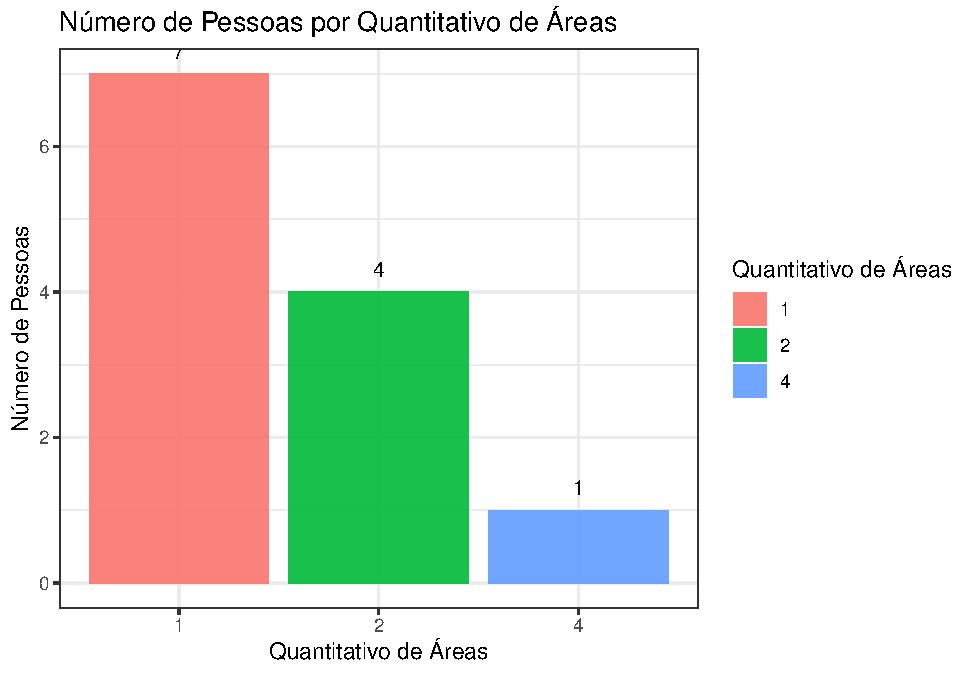
\includegraphics{LuanFreitas.relatorio2_files/figure-latex/unnamed-chunk-78-1.pdf}

O gráfico ilustra quantidade de orientações de mestrado por quantitativo
de professores:

\begin{Shaded}
\begin{Highlighting}[]
\NormalTok{profile }\OperatorTok
\StringTok{  }\KeywordTok{sapply}\NormalTok{(}\ControlFlowTok{function}\NormalTok{(x)}
    \KeywordTok{length}\NormalTok{(x}\OperatorTok{$}\NormalTok{orientacoes_academicas}\OperatorTok{$}\NormalTok{ORIENTACAO_CONCLUIDA_MESTRADO}\OperatorTok{$}\NormalTok{ano)) }\OperatorTok
\StringTok{  }\KeywordTok{unlist}\NormalTok{() }\OperatorTok\StringTok{ }\KeywordTok{table}\NormalTok{() }\OperatorTok\StringTok{ }\KeywordTok{rev}\NormalTok{() }\OperatorTok\StringTok{ }\KeywordTok{as.data.frame}\NormalTok{() }\OperatorTok
\StringTok{  }\KeywordTok{ggplot}\NormalTok{(}\KeywordTok{aes}\NormalTok{(}\DataTypeTok{x =}\NormalTok{ ., }\DataTypeTok{y =}\NormalTok{ Freq)) }\OperatorTok{+}\StringTok{ }\KeywordTok{geom_col}\NormalTok{(}\DataTypeTok{fill =} \StringTok{"blue4"}\NormalTok{, }\DataTypeTok{width =} \FloatTok{0.5}\NormalTok{) }\OperatorTok{+}\StringTok{ }\KeywordTok{coord_flip}\NormalTok{() }\OperatorTok{+}
\StringTok{  }\KeywordTok{labs}\NormalTok{(}\DataTypeTok{title =} \StringTok{"N昼㹡mero de Orienta攼㸷昼㸵es de Mestrado por Quantitativo de pessoas"}\NormalTok{,}
       \DataTypeTok{y =} \StringTok{"Pessoas"}\NormalTok{, }\DataTypeTok{x =} \StringTok{"Orienta攼㸷昼㸵es"}\NormalTok{) }\OperatorTok{+}\StringTok{ }\KeywordTok{scale_y_continuous}\NormalTok{(}\DataTypeTok{limits =} \KeywordTok{c}\NormalTok{(}\DecValTok{0}\NormalTok{, }\DecValTok{400}\NormalTok{)) }\OperatorTok{+}
\StringTok{  }\KeywordTok{theme_bw}\NormalTok{() }\OperatorTok{+}
\StringTok{  }\KeywordTok{geom_text}\NormalTok{(}\KeywordTok{aes}\NormalTok{(}\DataTypeTok{label =}\NormalTok{ Freq),}
            \DataTypeTok{hjust =} \FloatTok{-0.3}\NormalTok{,}
            \DataTypeTok{vjust =} \FloatTok{0.3}\NormalTok{,}
            \DataTypeTok{size =} \FloatTok{3.1}\NormalTok{)}
\end{Highlighting}
\end{Shaded}

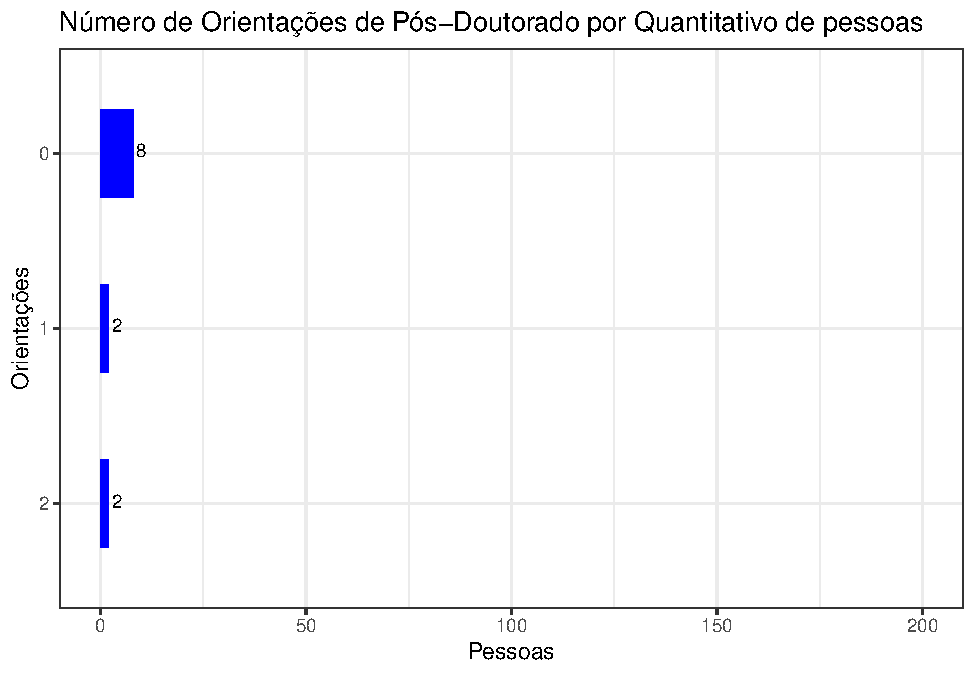
\includegraphics{LuanFreitas.relatorio2_files/figure-latex/unnamed-chunk-79-1.pdf}

O gráfico ilustra a quantidade de orientações de doutorado por
quantitativo de professores:

\begin{Shaded}
\begin{Highlighting}[]
\NormalTok{profile }\OperatorTok
\StringTok{  }\KeywordTok{sapply}\NormalTok{(}\ControlFlowTok{function}\NormalTok{(x)}
    \KeywordTok{length}\NormalTok{(}
\NormalTok{      x}\OperatorTok{$}\NormalTok{orientacoes_academicas}\OperatorTok{$}\NormalTok{ORIENTACAO_CONCLUIDA_DOUTORADO}\OperatorTok{$}\NormalTok{ano}
\NormalTok{    )) }\OperatorTok
\StringTok{  }\KeywordTok{unlist}\NormalTok{() }\OperatorTok\StringTok{ }\KeywordTok{table}\NormalTok{() }\OperatorTok\StringTok{ }\KeywordTok{rev}\NormalTok{() }\OperatorTok\StringTok{ }\KeywordTok{as.data.frame}\NormalTok{() }\OperatorTok
\StringTok{  }\KeywordTok{ggplot}\NormalTok{(}\KeywordTok{aes}\NormalTok{(}\DataTypeTok{x =}\NormalTok{ ., }\DataTypeTok{y =}\NormalTok{ Freq)) }\OperatorTok{+}\StringTok{ }\KeywordTok{geom_col}\NormalTok{(}\DataTypeTok{fill =} \StringTok{"blue"}\NormalTok{, }\DataTypeTok{width =} \FloatTok{0.5}\NormalTok{) }\OperatorTok{+}\StringTok{ }\KeywordTok{coord_flip}\NormalTok{() }\OperatorTok{+}
\StringTok{  }\KeywordTok{labs}\NormalTok{(}\DataTypeTok{title =} \StringTok{"N昼㹡mero de Orienta攼㸷昼㸵es de Doutorado por Quantitativo de pessoas"}\NormalTok{,}
       \DataTypeTok{y =} \StringTok{"Pessoas"}\NormalTok{, }\DataTypeTok{x =} \StringTok{"Orienta攼㸷昼㸵es"}\NormalTok{) }\OperatorTok{+}\StringTok{ }\KeywordTok{scale_y_continuous}\NormalTok{(}\DataTypeTok{limits =} \KeywordTok{c}\NormalTok{(}\DecValTok{0}\NormalTok{, }\DecValTok{300}\NormalTok{)) }\OperatorTok{+}
\StringTok{  }\KeywordTok{theme_bw}\NormalTok{() }\OperatorTok{+}
\StringTok{  }\KeywordTok{geom_text}\NormalTok{(}\KeywordTok{aes}\NormalTok{(}\DataTypeTok{label =}\NormalTok{ Freq),}
            \DataTypeTok{hjust =} \FloatTok{-0.3}\NormalTok{,}
            \DataTypeTok{vjust =} \FloatTok{0.3}\NormalTok{,}
            \DataTypeTok{size =} \FloatTok{3.1}\NormalTok{)}
\end{Highlighting}
\end{Shaded}

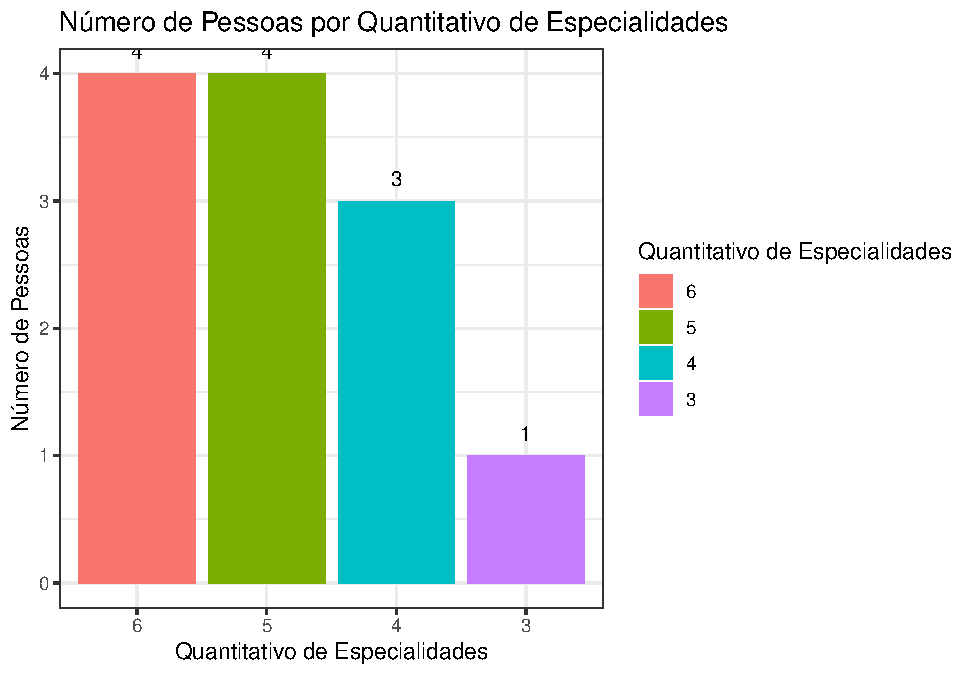
\includegraphics{LuanFreitas.relatorio2_files/figure-latex/unnamed-chunk-80-1.pdf}

O gráfico ilustra a quantidade de orientações de pós-doutorado por
quantitativo de professores:

\begin{Shaded}
\begin{Highlighting}[]
\NormalTok{profile }\OperatorTok
\StringTok{  }\KeywordTok{sapply}\NormalTok{(}
    \ControlFlowTok{function}\NormalTok{(x)}
      \KeywordTok{length}\NormalTok{(}
\NormalTok{        x}\OperatorTok{$}\NormalTok{orientacoes_academicas}\OperatorTok{$}\NormalTok{ORIENTACAO_CONCLUIDA_POS_DOUTORADO}\OperatorTok{$}\NormalTok{ano}
\NormalTok{      )}
\NormalTok{  ) }\OperatorTok
\StringTok{  }\KeywordTok{unlist}\NormalTok{() }\OperatorTok\StringTok{ }\KeywordTok{table}\NormalTok{() }\OperatorTok\StringTok{ }\KeywordTok{rev}\NormalTok{() }\OperatorTok\StringTok{ }\KeywordTok{as.data.frame}\NormalTok{() }\OperatorTok
\StringTok{  }\KeywordTok{ggplot}\NormalTok{(}\KeywordTok{aes}\NormalTok{(}\DataTypeTok{x =}\NormalTok{ ., }\DataTypeTok{y =}\NormalTok{ Freq)) }\OperatorTok{+}\StringTok{ }\KeywordTok{geom_col}\NormalTok{(}\DataTypeTok{fill =} \StringTok{"blue"}\NormalTok{, }\DataTypeTok{width =} \FloatTok{0.5}\NormalTok{) }\OperatorTok{+}\StringTok{ }\KeywordTok{coord_flip}\NormalTok{() }\OperatorTok{+}
\StringTok{  }\KeywordTok{labs}\NormalTok{(}\DataTypeTok{title =} \StringTok{"N昼㹡mero de Orienta攼㸷昼㸵es de P昼㸳s-Doutorado por Quantitativo de pessoas"}\NormalTok{,}
       \DataTypeTok{y =} \StringTok{"Pessoas"}\NormalTok{, }\DataTypeTok{x =} \StringTok{"Orienta攼㸷昼㸵es"}\NormalTok{) }\OperatorTok{+}\StringTok{ }\KeywordTok{scale_y_continuous}\NormalTok{(}\DataTypeTok{limits =} \KeywordTok{c}\NormalTok{(}\DecValTok{0}\NormalTok{, }\DecValTok{200}\NormalTok{)) }\OperatorTok{+}
\StringTok{  }\KeywordTok{theme_bw}\NormalTok{() }\OperatorTok{+}
\StringTok{  }\KeywordTok{geom_text}\NormalTok{(}\KeywordTok{aes}\NormalTok{(}\DataTypeTok{label =}\NormalTok{ Freq),}
            \DataTypeTok{hjust =} \FloatTok{-0.3}\NormalTok{,}
            \DataTypeTok{vjust =} \FloatTok{0.3}\NormalTok{,}
            \DataTypeTok{size =} \FloatTok{3.1}\NormalTok{)}
\end{Highlighting}
\end{Shaded}

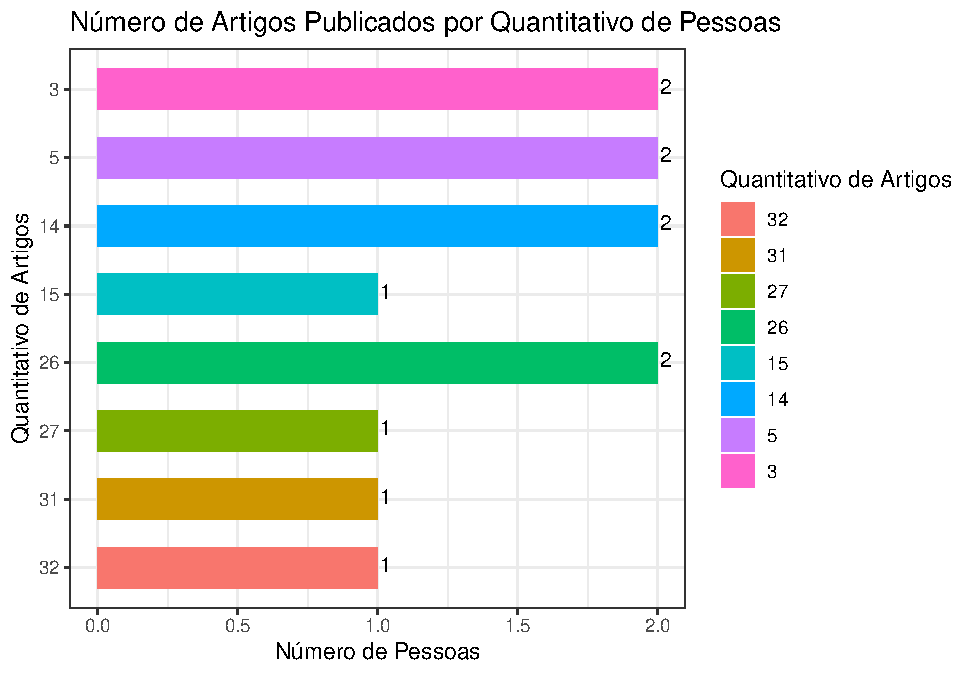
\includegraphics{LuanFreitas.relatorio2_files/figure-latex/unnamed-chunk-81-1.pdf}

O gráfico ilustra as as relações de Orientações Concluídas e
Publicações:

\begin{Shaded}
\begin{Highlighting}[]
\NormalTok{profile.areas }\OperatorTok
\StringTok{  }\KeywordTok{select}\NormalTok{(}\OperatorTok{-}\NormalTok{sub_area, }\OperatorTok{-}\NormalTok{especialidade) }\OperatorTok
\StringTok{  }\KeywordTok{distinct}\NormalTok{() }\OperatorTok
\StringTok{  }\KeywordTok{group_by}\NormalTok{(publicacoes) }\OperatorTok
\StringTok{  }\KeywordTok{ggplot}\NormalTok{(}\KeywordTok{aes}\NormalTok{(publicacoes, orientacoes_concluidas, }\DataTypeTok{color =}\NormalTok{ area)) }\OperatorTok{+}
\StringTok{  }\KeywordTok{geom_point}\NormalTok{(}\DataTypeTok{shape =} \DecValTok{2}\NormalTok{, }\DataTypeTok{size =} \FloatTok{.8}\NormalTok{) }\OperatorTok{+}\StringTok{ }\KeywordTok{geom_jitter}\NormalTok{(}\DataTypeTok{shape =} \DecValTok{2}\NormalTok{, }\DataTypeTok{size =} \FloatTok{.8}\NormalTok{) }\OperatorTok{+}
\StringTok{  }\KeywordTok{ggtitle}\NormalTok{(}\StringTok{'Rela攼㸷攼㸳o de Orienta攼㸷昼㸵es Conclu攼㹤das e Publica攼㸷昼㸵es'}\NormalTok{) }\OperatorTok{+}
\StringTok{  }\KeywordTok{labs}\NormalTok{(}\DataTypeTok{x =} \StringTok{'Publica攼㸷昼㸵es'}\NormalTok{, }\DataTypeTok{y =} \StringTok{'Orienta攼㸷昼㸵es conclu攼㹤das'}\NormalTok{) }\OperatorTok{+}\StringTok{ }\KeywordTok{facet_wrap}\NormalTok{(. }\OperatorTok{~}\StringTok{ }\NormalTok{grande_area, }\DataTypeTok{ncol =} \DecValTok{2}\NormalTok{)}
\end{Highlighting}
\end{Shaded}

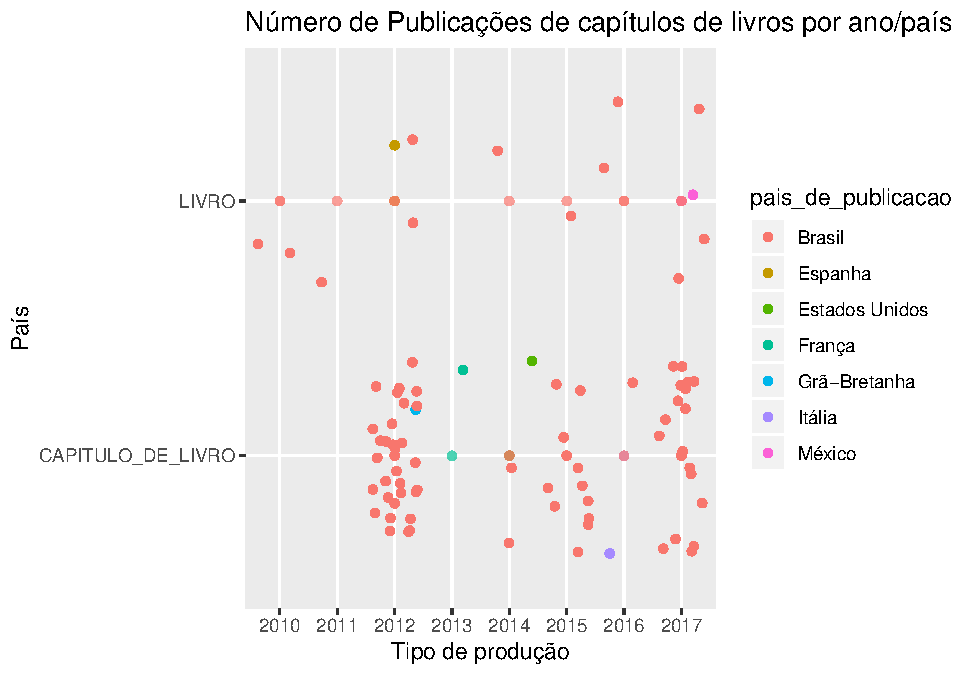
\includegraphics{LuanFreitas.relatorio2_files/figure-latex/unnamed-chunk-82-1.pdf}

O gráfico ilustra a quantidade de orientações completas por ano (em
forma de linhas e pontos):

\begin{Shaded}
\begin{Highlighting}[]
\NormalTok{profile.df.orientacoes <-}\StringTok{ }\KeywordTok{extrai.orientacoes}\NormalTok{(profile) }\OperatorTok
\StringTok{  }\KeywordTok{select}\NormalTok{(id_lattes_orientadores, natureza, ano, orientacao, }\KeywordTok{everything}\NormalTok{()) }\OperatorTok
\StringTok{  }\KeywordTok{mutate}\NormalTok{(}\DataTypeTok{Status =} \KeywordTok{ifelse}\NormalTok{(}\KeywordTok{grepl}\NormalTok{(}\StringTok{"CONCLUIDA"}\NormalTok{, orientacao), }\StringTok{"Conclu攼㹤da"}\NormalTok{, }\StringTok{"Em andamento"}\NormalTok{)) }\OperatorTok
\StringTok{  }\KeywordTok{mutate}\NormalTok{(}\DataTypeTok{Natureza =} \KeywordTok{case_when}\NormalTok{(}\KeywordTok{grepl}\NormalTok{(}\StringTok{"MESTRADO"}\NormalTok{, }\KeywordTok{str_to_upper}\NormalTok{(natureza)) }\OperatorTok{~}\StringTok{ "Mestrado"}\NormalTok{,}
                              \KeywordTok{grepl}\NormalTok{(}\StringTok{"P搼㸳S-DOUTORADO"}\NormalTok{, }\KeywordTok{str_to_upper}\NormalTok{(natureza)) }\OperatorTok{~}\StringTok{ "P昼㸳s-doutorado"}\NormalTok{,}
                              \KeywordTok{grepl}\NormalTok{(}\StringTok{"DOUTORADO"}\NormalTok{, }\KeywordTok{str_to_upper}\NormalTok{(natureza)) }\OperatorTok{~}\StringTok{ "Doutorado"}\NormalTok{,}
                              \KeywordTok{grepl}\NormalTok{(}\StringTok{"INICIACAO"}\NormalTok{, }\KeywordTok{str_to_upper}\NormalTok{(natureza)) }\OperatorTok{~}\StringTok{ "Inicia攼㸷攼㸳o Cient攼㹤fica"}\NormalTok{,}
                              \KeywordTok{grepl}\NormalTok{(}\StringTok{"INICIA挼㸷挼㸳O"}\NormalTok{, }\KeywordTok{str_to_upper}\NormalTok{(natureza)) }\OperatorTok{~}\StringTok{ "Inicia攼㸷攼㸳o Cient攼㹤fica"}\NormalTok{,}
                              \OtherTok{TRUE} \OperatorTok{~}\StringTok{ "Outras naturezas"}\NormalTok{))}

\NormalTok{profile.df.orientacoes }\OperatorTok\StringTok{ }\KeywordTok{group_by}\NormalTok{(ano, Status) }\OperatorTok
\StringTok{  }\KeywordTok{ggplot}\NormalTok{(}\KeywordTok{aes}\NormalTok{(}\DataTypeTok{x =}\NormalTok{ ano, }\DataTypeTok{y =}\NormalTok{ Status, }\DataTypeTok{color =}\NormalTok{ Status)) }\OperatorTok{+}
\StringTok{  }\KeywordTok{labs}\NormalTok{(}\DataTypeTok{title =} \StringTok{"Natureza das orienta攼㸷昼㸵es por tipo de orienta攼㸷攼㸳o"}\NormalTok{) }\OperatorTok{+}
\StringTok{  }\KeywordTok{geom_point}\NormalTok{(}\DataTypeTok{shape =} \DecValTok{1}\NormalTok{) }\OperatorTok{+}\StringTok{ }\KeywordTok{geom_jitter}\NormalTok{(}\DataTypeTok{shape =} \DecValTok{1}\NormalTok{) }\OperatorTok{+}\StringTok{ }\KeywordTok{facet_wrap}\NormalTok{(. }\OperatorTok{~}\StringTok{ }\NormalTok{Natureza)}
\end{Highlighting}
\end{Shaded}

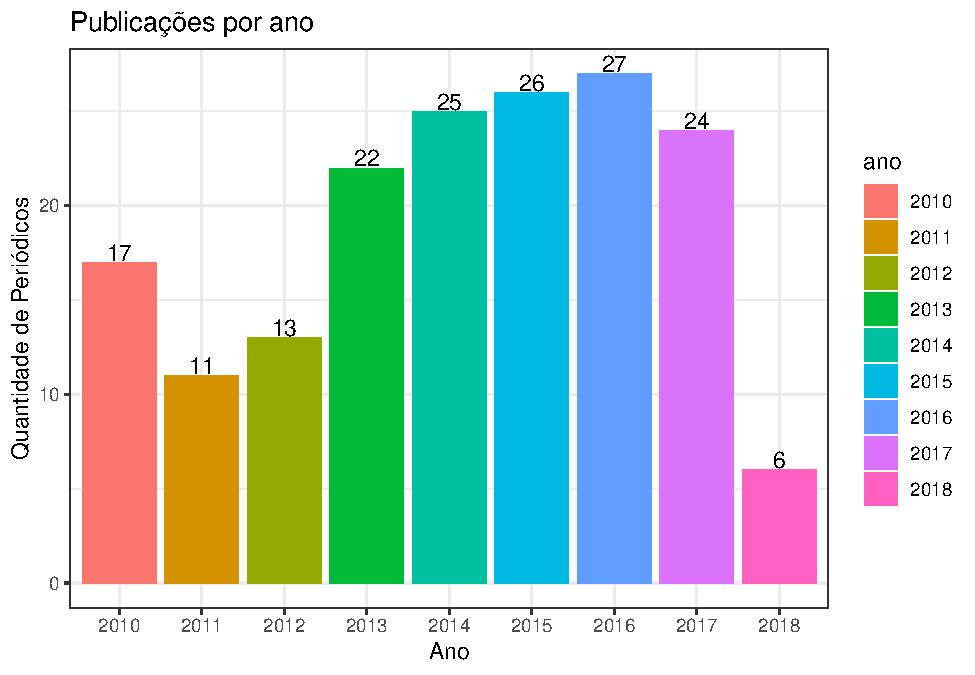
\includegraphics{LuanFreitas.relatorio2_files/figure-latex/unnamed-chunk-83-1.pdf}

O gráfico ilustra a quantidade publicações de capítulos de livros por
ano/país:

\begin{Shaded}
\begin{Highlighting}[]
\NormalTok{profile.df.publicacoes }\OperatorTok
\StringTok{  }\KeywordTok{filter}\NormalTok{((tipo_producao }\OperatorTok\StringTok{ }\KeywordTok{c}\NormalTok{(}\StringTok{'LIVRO'}\NormalTok{, }\StringTok{'CAPITULO_DE_LIVRO'}\NormalTok{))) }\OperatorTok
\StringTok{  }\KeywordTok{group_by}\NormalTok{(tipo_producao, pais_de_publicacao) }\OperatorTok
\StringTok{  }\KeywordTok{ggplot}\NormalTok{(}\KeywordTok{aes}\NormalTok{(ano, tipo_producao, }\DataTypeTok{col =}\NormalTok{ pais_de_publicacao)) }\OperatorTok{+}
\StringTok{  }\KeywordTok{labs}\NormalTok{(}\DataTypeTok{title =} \StringTok{"N昼㹡mero de Publica攼㸷昼㸵es de cap攼㹤tulos de livros por ano/pa攼㹤s"}\NormalTok{) }\OperatorTok{+}
\StringTok{  }\KeywordTok{geom_point}\NormalTok{(}\DataTypeTok{alpha =} \FloatTok{0.7}\NormalTok{) }\OperatorTok{+}\StringTok{ }\KeywordTok{geom_jitter}\NormalTok{() }\OperatorTok{+}
\StringTok{  }\KeywordTok{labs}\NormalTok{(}\DataTypeTok{x =} \StringTok{'Tipo de produ攼㸷攼㸳o'}\NormalTok{, }\DataTypeTok{y =} \StringTok{'Pa攼㹤s'}\NormalTok{)}
\end{Highlighting}
\end{Shaded}

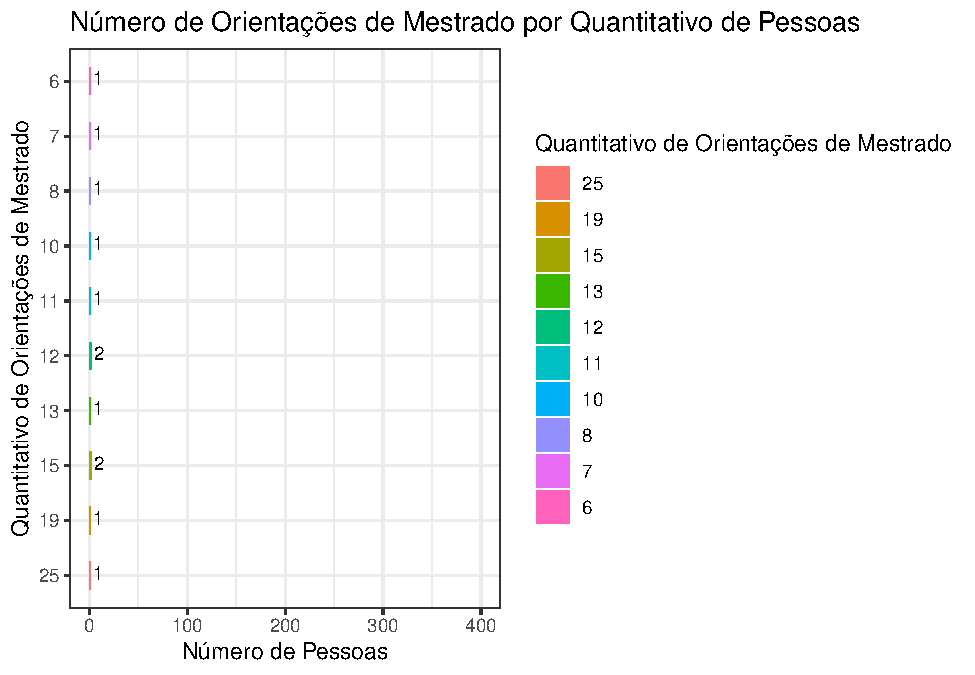
\includegraphics{LuanFreitas.relatorio2_files/figure-latex/unnamed-chunk-84-1.pdf}

\hypertarget{arquivo-publicauxe7uxe3o-1}{%
\subsubsection{Arquivo Publicação}\label{arquivo-publicauxe7uxe3o-1}}

O gráfico ilustra a quantidade de publicações por ano:

\begin{Shaded}
\begin{Highlighting}[]
\NormalTok{publication.periodico.df }\OperatorTok
\StringTok{  }\KeywordTok{ggplot}\NormalTok{(}\KeywordTok{aes}\NormalTok{(}\DataTypeTok{x =}\NormalTok{ ano)) }\OperatorTok{+}\StringTok{ }\KeywordTok{geom_bar}\NormalTok{(}\KeywordTok{aes}\NormalTok{(}\DataTypeTok{fill =}\NormalTok{ ano)) }\OperatorTok{+}
\StringTok{  }\KeywordTok{geom_text}\NormalTok{(}\DataTypeTok{stat =} \StringTok{"count"}\NormalTok{, }\KeywordTok{aes}\NormalTok{(}\DataTypeTok{label =} \KeywordTok{formatC}\NormalTok{(..count.., }\DataTypeTok{big.mark =} \StringTok{","}\NormalTok{)), }\DataTypeTok{vjust =}
              \FloatTok{-0.1}\NormalTok{) }\OperatorTok{+}
\StringTok{  }\KeywordTok{theme_bw}\NormalTok{() }\OperatorTok{+}\StringTok{ }\KeywordTok{labs}\NormalTok{(}\DataTypeTok{title =} \StringTok{"Publica攼㸷昼㸵es por ano"}\NormalTok{, }\DataTypeTok{x =} \StringTok{"Ano"}\NormalTok{, }\DataTypeTok{y =} \StringTok{"Quantidade de Peri昼㸳dicos"}\NormalTok{) }\OperatorTok{+}
\StringTok{  }\KeywordTok{scale_y_continuous}\NormalTok{(}\DataTypeTok{labels =}\NormalTok{ comma)}
\end{Highlighting}
\end{Shaded}

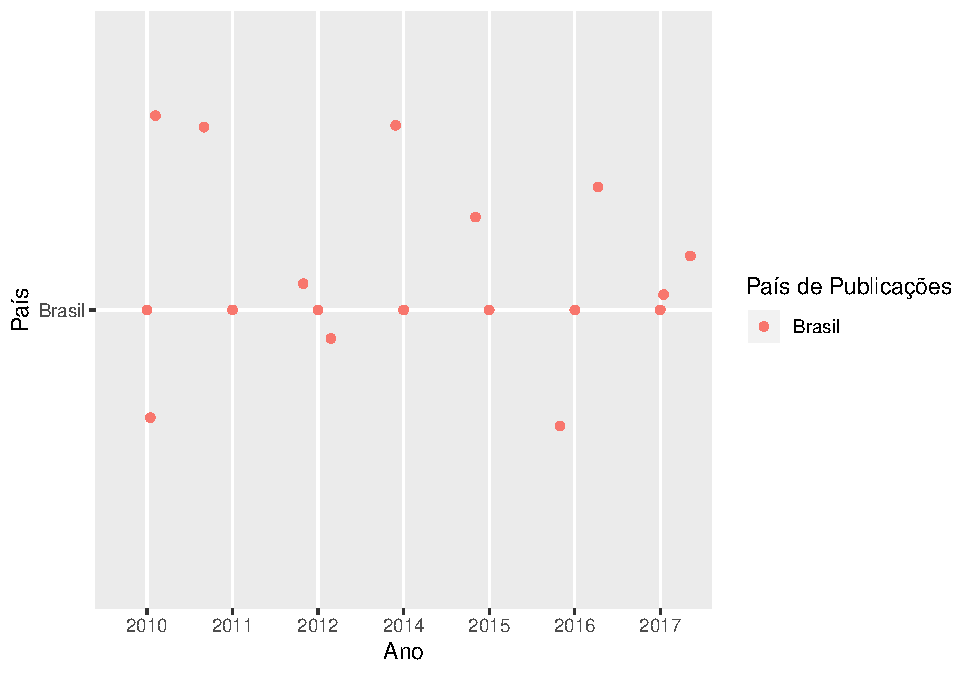
\includegraphics{LuanFreitas.relatorio2_files/figure-latex/unnamed-chunk-86-1.pdf}

O gráfico ilustra as 20 revistas publicadas mais publicadas:

\begin{Shaded}
\begin{Highlighting}[]
\NormalTok{publication.periodico.df }\OperatorTok\StringTok{ }\KeywordTok{select}\NormalTok{(periodico) }\OperatorTok\StringTok{ }\KeywordTok{table}\NormalTok{() }\OperatorTok\StringTok{ }\KeywordTok{as.data.frame}\NormalTok{() }\OperatorTok\StringTok{ }\KeywordTok{arrange}\NormalTok{(}\KeywordTok{desc}\NormalTok{(Freq)) }\OperatorTok
\StringTok{  }\KeywordTok{head}\NormalTok{(}\DecValTok{20}\NormalTok{) }\OperatorTok\StringTok{ }\KeywordTok{ggplot}\NormalTok{(}\KeywordTok{aes}\NormalTok{(}\DataTypeTok{x =} \KeywordTok{reorder}\NormalTok{(., (Freq)), }\DataTypeTok{y =}\NormalTok{ Freq)) }\OperatorTok{+}\StringTok{ }\KeywordTok{geom_col}\NormalTok{(}\DataTypeTok{fill =} \StringTok{"red4"}\NormalTok{) }\OperatorTok{+}\StringTok{ }\KeywordTok{coord_flip}\NormalTok{() }\OperatorTok{+}
\StringTok{  }\KeywordTok{labs}\NormalTok{(}\DataTypeTok{title =} \StringTok{"Os 20 Peri昼㸳dicos com Maior Publica攼㸷昼㸵es"}\NormalTok{,}
       \DataTypeTok{y =} \StringTok{"N昼㹡mero de Publica攼㸷昼㸵es"}\NormalTok{, }\DataTypeTok{x =} \StringTok{"Revistas"}\NormalTok{) }\OperatorTok{+}\StringTok{ }\KeywordTok{geom_text}\NormalTok{(}
         \KeywordTok{aes}\NormalTok{(}\DataTypeTok{label =} \KeywordTok{comma}\NormalTok{(Freq)),}
         \DataTypeTok{hjust =} \FloatTok{-0.2}\NormalTok{,}
         \DataTypeTok{vjust =} \FloatTok{0.3}\NormalTok{,}
         \DataTypeTok{size =} \FloatTok{3.5}
\NormalTok{       ) }\OperatorTok{+}\StringTok{ }\KeywordTok{theme_bw}\NormalTok{() }\OperatorTok{+}
\StringTok{  }\KeywordTok{scale_y_continuous}\NormalTok{(}\DataTypeTok{limits =} \KeywordTok{c}\NormalTok{(}\DecValTok{0}\NormalTok{, }\DecValTok{400}\NormalTok{))}
\end{Highlighting}
\end{Shaded}

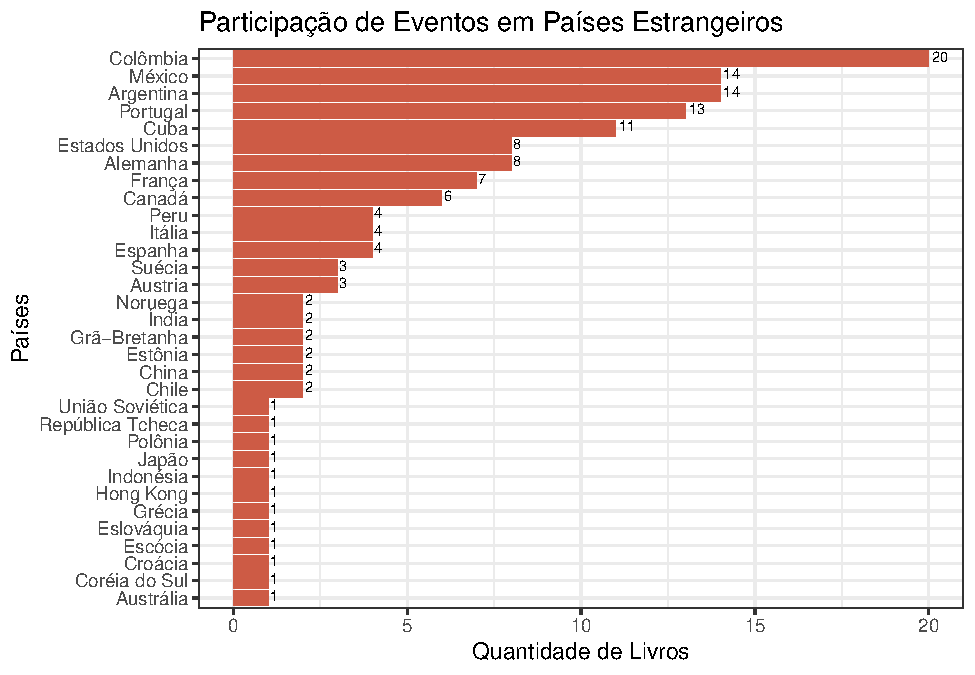
\includegraphics{LuanFreitas.relatorio2_files/figure-latex/unnamed-chunk-87-1.pdf}

O gráfico ilustra a quantidade de publicações de livros em países
estrangeiros (em forma de colunas):

\begin{Shaded}
\begin{Highlighting}[]
\NormalTok{publication.livros.df }\OperatorTok
\StringTok{  }\KeywordTok{group_by}\NormalTok{(pais_de_publicacao) }\OperatorTok
\StringTok{  }\KeywordTok{summarise}\NormalTok{(}\DataTypeTok{Quantidade =} \KeywordTok{n}\NormalTok{()) }\OperatorTok
\StringTok{  }\KeywordTok{filter}\NormalTok{(pais_de_publicacao }\OperatorTok{!=}\StringTok{ "Brasil"}\NormalTok{) }\OperatorTok
\StringTok{  }\KeywordTok{ggplot}\NormalTok{(}\KeywordTok{aes}\NormalTok{(}\DataTypeTok{x =} \KeywordTok{reorder}\NormalTok{(pais_de_publicacao, (Quantidade)), }\DataTypeTok{y =}\NormalTok{ Quantidade)) }\OperatorTok{+}
\StringTok{  }\KeywordTok{geom_col}\NormalTok{(}\DataTypeTok{fill =} \StringTok{"coral"}\NormalTok{) }\OperatorTok{+}\StringTok{ }\KeywordTok{geom_text}\NormalTok{(}
    \KeywordTok{aes}\NormalTok{(}\DataTypeTok{label =} \KeywordTok{comma}\NormalTok{(Quantidade)),}
    \DataTypeTok{hjust =} \FloatTok{-0.2}\NormalTok{,}
    \DataTypeTok{vjust =} \FloatTok{0.3}\NormalTok{,}
    \DataTypeTok{size =} \FloatTok{3.5}
\NormalTok{  ) }\OperatorTok{+}\StringTok{ }\KeywordTok{coord_flip}\NormalTok{() }\OperatorTok{+}
\StringTok{  }\KeywordTok{labs}\NormalTok{(}\DataTypeTok{title =} \StringTok{"Publica攼㸷昼㸵es de Livros em Pa攼㹤ses Estrangeiros"}\NormalTok{, }\DataTypeTok{x =} \StringTok{"Pa攼㹤ses"}\NormalTok{, }\DataTypeTok{y =} \StringTok{"Quantidade de Livros"}\NormalTok{) }\OperatorTok{+}
\StringTok{  }\KeywordTok{theme_bw}\NormalTok{()}
\end{Highlighting}
\end{Shaded}

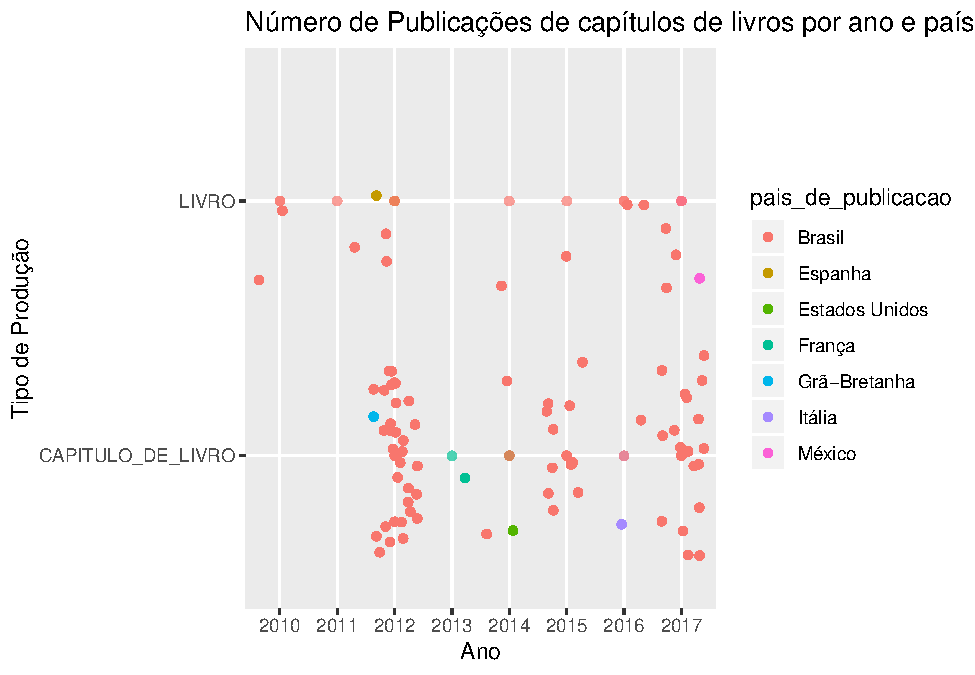
\includegraphics{LuanFreitas.relatorio2_files/figure-latex/unnamed-chunk-88-1.pdf}

O gráfico ilustra a quantidade de publicações de livros no Brasil (em
forma de pontos):

\begin{Shaded}
\begin{Highlighting}[]
\NormalTok{publication.livros.df }\OperatorTok
\StringTok{  }\KeywordTok{filter}\NormalTok{(}
\NormalTok{    pais_de_publicacao }\OperatorTok\StringTok{ }\KeywordTok{c}\NormalTok{(}
      \StringTok{"Brasil"}\NormalTok{,}
      \StringTok{"Estados Unidos"}\NormalTok{,}
      \StringTok{"Holanda"}\NormalTok{,}
      \StringTok{"Gr攼㸳-Bretanha"}\NormalTok{,}
      \StringTok{"Alemanha"}\NormalTok{,}
      \StringTok{"Sui攼㸷a"}
\NormalTok{    )}
\NormalTok{  ) }\OperatorTok
\StringTok{  }\KeywordTok{group_by}\NormalTok{(ano, pais_de_publicacao) }\OperatorTok
\StringTok{  }\KeywordTok{ggplot}\NormalTok{(}\KeywordTok{aes}\NormalTok{(}\DataTypeTok{x =}\NormalTok{ ano, }\DataTypeTok{y =}\NormalTok{ pais_de_publicacao, }\DataTypeTok{color =}\NormalTok{ pais_de_publicacao)) }\OperatorTok{+}
\StringTok{  }\KeywordTok{xlab}\NormalTok{(}\StringTok{"Ano"}\NormalTok{) }\OperatorTok{+}\StringTok{ }\KeywordTok{ylab}\NormalTok{(}\StringTok{"Pa攼㹤s"}\NormalTok{) }\OperatorTok{+}\StringTok{ }\KeywordTok{geom_point}\NormalTok{() }\OperatorTok{+}\StringTok{ }\KeywordTok{geom_jitter}\NormalTok{() }\OperatorTok{+}
\StringTok{  }\KeywordTok{labs}\NormalTok{(}\DataTypeTok{color =} \StringTok{"Pa攼㹤s de Publica攼㸷昼㸵es"}\NormalTok{)}
\end{Highlighting}
\end{Shaded}

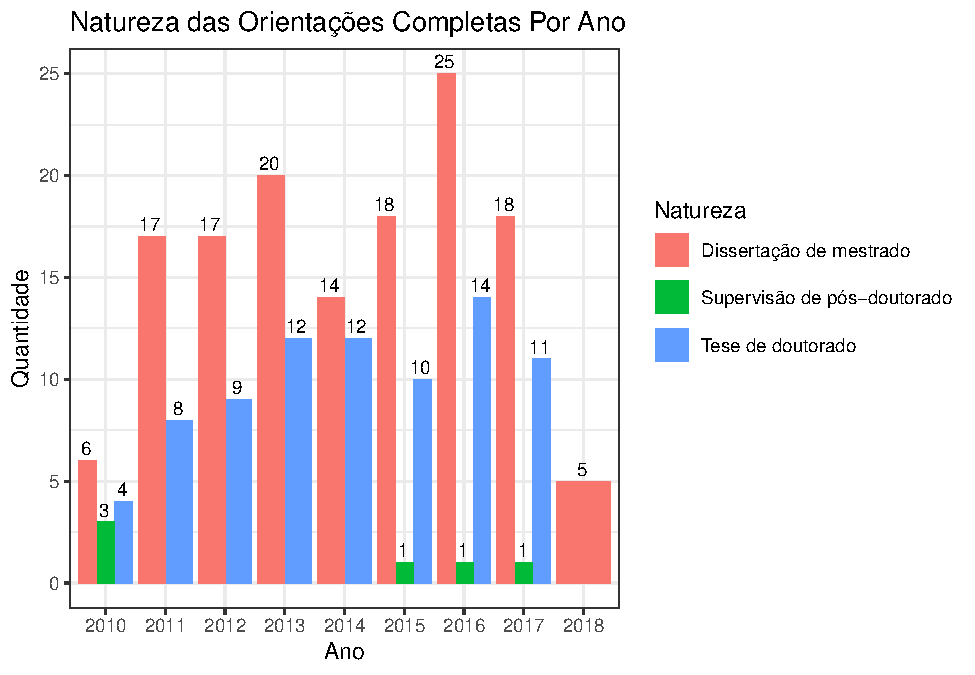
\includegraphics{LuanFreitas.relatorio2_files/figure-latex/unnamed-chunk-89-1.pdf}

O gráfico ilustra a quantidade de participação de eventos de livros em
países estrangeiros:

\begin{Shaded}
\begin{Highlighting}[]
\NormalTok{publication.eventos.df }\OperatorTok
\StringTok{  }\KeywordTok{group_by}\NormalTok{(pais_do_evento) }\OperatorTok
\StringTok{  }\KeywordTok{summarise}\NormalTok{(}\DataTypeTok{Quantidade =} \KeywordTok{n}\NormalTok{()) }\OperatorTok
\StringTok{  }\KeywordTok{filter}\NormalTok{(pais_do_evento }\OperatorTok{!=}\StringTok{ "Brasil"}\NormalTok{) }\OperatorTok
\StringTok{  }\KeywordTok{ggplot}\NormalTok{(}\KeywordTok{aes}\NormalTok{(}\DataTypeTok{x =} \KeywordTok{reorder}\NormalTok{(pais_do_evento, (Quantidade)), }\DataTypeTok{y =}\NormalTok{ Quantidade)) }\OperatorTok{+}
\StringTok{  }\KeywordTok{geom_col}\NormalTok{(}\DataTypeTok{fill =} \StringTok{"coral3"}\NormalTok{) }\OperatorTok{+}\StringTok{ }\KeywordTok{geom_text}\NormalTok{(}
    \KeywordTok{aes}\NormalTok{(}\DataTypeTok{label =} \KeywordTok{comma}\NormalTok{(Quantidade)),}
    \DataTypeTok{hjust =} \FloatTok{-0.2}\NormalTok{,}
    \DataTypeTok{vjust =} \FloatTok{0.3}\NormalTok{,}
    \DataTypeTok{size =} \FloatTok{2.5}
\NormalTok{  ) }\OperatorTok{+}\StringTok{ }\KeywordTok{coord_flip}\NormalTok{() }\OperatorTok{+}
\StringTok{  }\KeywordTok{labs}\NormalTok{(}\DataTypeTok{title =} \StringTok{"Participa攼㸷攼㸳o de Eventos em Pa攼㹤ses Estrangeiros"}\NormalTok{, }\DataTypeTok{x =} \StringTok{"Pa攼㹤ses"}\NormalTok{, }\DataTypeTok{y =} \StringTok{"Quantidade de Livros"}\NormalTok{) }\OperatorTok{+}
\StringTok{  }\KeywordTok{theme_bw}\NormalTok{()}
\end{Highlighting}
\end{Shaded}

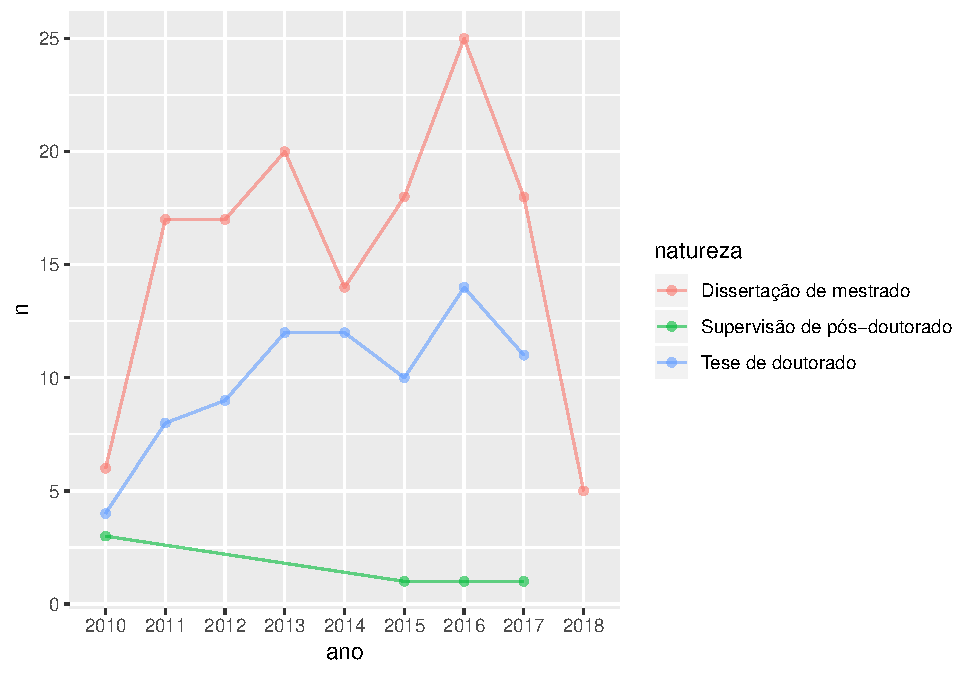
\includegraphics{LuanFreitas.relatorio2_files/figure-latex/unnamed-chunk-90-1.pdf}

\hypertarget{arquivo-orientauxe7uxe3o-1}{%
\subsubsection{Arquivo Orientação}\label{arquivo-orientauxe7uxe3o-1}}

O gráfico ilustra a quantidade de orientações completas por ano (em
forma de barras):

\begin{Shaded}
\begin{Highlighting}[]
\KeywordTok{ggplot}\NormalTok{(orient.df, }\KeywordTok{aes}\NormalTok{(ano, }\DataTypeTok{fill =} \KeywordTok{factor}\NormalTok{(natureza))) }\OperatorTok{+}
\StringTok{  }\KeywordTok{geom_bar}\NormalTok{(}\DataTypeTok{stat =} \StringTok{"count"}\NormalTok{, }\DataTypeTok{position =} \StringTok{"dodge"}\NormalTok{) }\OperatorTok{+}
\StringTok{  }\KeywordTok{ggtitle}\NormalTok{(}\StringTok{"Natureza das Orienta攼㸷昼㸵es Completas Por Ano"}\NormalTok{) }\OperatorTok{+}
\StringTok{  }\KeywordTok{theme}\NormalTok{(}\DataTypeTok{legend.position =} \StringTok{"right"}\NormalTok{, }\DataTypeTok{legend.text =} \KeywordTok{element_text}\NormalTok{(}\DataTypeTok{size =} \DecValTok{7}\NormalTok{)) }\OperatorTok{+}
\StringTok{  }\KeywordTok{guides}\NormalTok{(}\DataTypeTok{fill =} \KeywordTok{guide_legend}\NormalTok{(}
    \DataTypeTok{nrow =} \DecValTok{5}\NormalTok{,}
    \DataTypeTok{byrow =} \OtherTok{TRUE}\NormalTok{,}
    \DataTypeTok{title.position =} \StringTok{"top"}
\NormalTok{  )) }\OperatorTok{+}
\StringTok{  }\KeywordTok{labs}\NormalTok{(}\DataTypeTok{x =} \StringTok{"Ano"}\NormalTok{, }\DataTypeTok{y =} \StringTok{"Quantidade"}\NormalTok{) }\OperatorTok{+}\StringTok{ }\KeywordTok{labs}\NormalTok{(}\DataTypeTok{fill =} \StringTok{"Natureza"}\NormalTok{) }\OperatorTok{+}\StringTok{ }\KeywordTok{theme_bw}\NormalTok{() }\OperatorTok{+}
\StringTok{  }\KeywordTok{geom_text}\NormalTok{(}
    \DataTypeTok{hjust =} \FloatTok{0.6}\NormalTok{,}
    \DataTypeTok{vjust =} \FloatTok{-0.4}\NormalTok{,}
    \DataTypeTok{size =} \DecValTok{3}\NormalTok{,}
    \DataTypeTok{color =} \StringTok{'black'}\NormalTok{,}
    \DataTypeTok{position =} \KeywordTok{position_dodge}\NormalTok{(}\DataTypeTok{width =} \FloatTok{0.9}\NormalTok{),}
    \DataTypeTok{stat =} \StringTok{"count"}\NormalTok{,}
    \KeywordTok{aes}\NormalTok{(}
      \DataTypeTok{group =} \KeywordTok{factor}\NormalTok{(natureza),}
      \DataTypeTok{label =} \KeywordTok{formatC}\NormalTok{(..count.., }\DataTypeTok{big.mark =} \StringTok{","}\NormalTok{)}
\NormalTok{    ),}
    \DataTypeTok{check_overlap =} \OtherTok{TRUE}
\NormalTok{  )}
\end{Highlighting}
\end{Shaded}

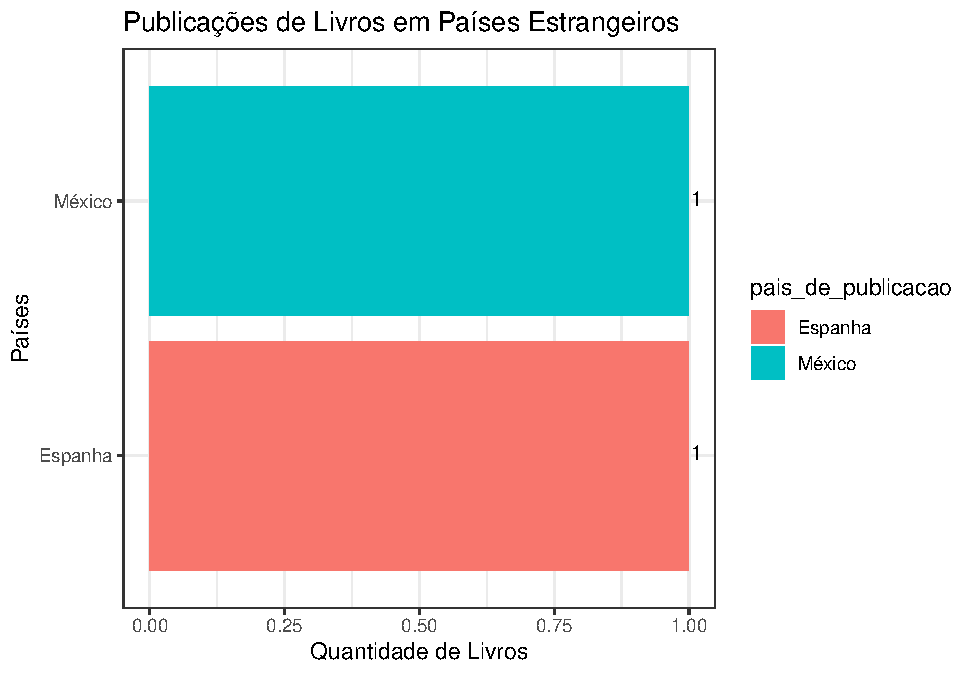
\includegraphics{LuanFreitas.relatorio2_files/figure-latex/unnamed-chunk-92-1.pdf}

O gráfico ilustra a quantidade de orientações completas por ano (em
forma de linhas e pontos):

\begin{Shaded}
\begin{Highlighting}[]
\KeywordTok{ggplot}\NormalTok{(orient_sum, }\KeywordTok{aes}\NormalTok{(}
  \DataTypeTok{x =}\NormalTok{ ano,}
  \DataTypeTok{y =}\NormalTok{ n,}
  \DataTypeTok{group =}\NormalTok{ natureza,}
  \DataTypeTok{color =}\NormalTok{ natureza}
\NormalTok{)) }\OperatorTok{+}
\StringTok{  }\KeywordTok{geom_line}\NormalTok{(}\DataTypeTok{alpha =} \FloatTok{0.6}\NormalTok{) }\OperatorTok{+}
\StringTok{  }\KeywordTok{geom_point}\NormalTok{(}\DataTypeTok{alpha =} \FloatTok{0.6}\NormalTok{)}
\end{Highlighting}
\end{Shaded}

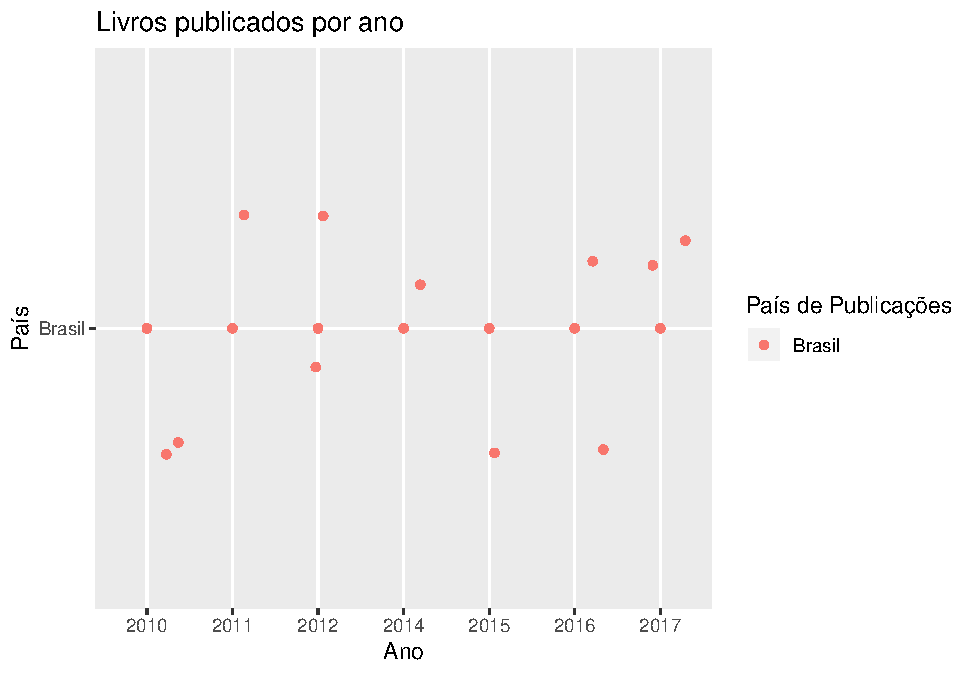
\includegraphics{LuanFreitas.relatorio2_files/figure-latex/unnamed-chunk-93-1.pdf}

\hypertarget{revisuxe3o-do-processo}{%
\subsection{Revisão do processo}\label{revisuxe3o-do-processo}}

Por meio das análises realizadas nas seções anteriores, tem-se que a
modelagem de análise com os modelos estatísticos foram adequados para
esse projeto, uma vez que permitiu a obtenção de resultados não triviais
em relação aos dois programas de pós-graduação analisados.

Tem-se ainda que os modelos e os datasets em que se aplicaram os modelos
nesse relatório são facilmente verificáveis e replicáveis por meio da
leitura desse documento.

\hypertarget{fase-6---implantauxe7uxe3o-deployment}{%
\section{Fase 6 - Implantação
(deployment)}\label{fase-6---implantauxe7uxe3o-deployment}}

Na fase de implantação, realiza-se o planejamento da implantação dos
scripts desenvolvidos para o ambiente operacional. Os scripts
desenvolvidos nesse trabalho permitem uma análise de dados do programa
de pós-graduação sob outros pontos de vista, que podem trazer
estatísticas e relações não triviais.

\hypertarget{conclusuxe3o}{%
\section{Conclusão}\label{conclusuxe3o}}

Esse trabalho mostrou uma forma de analisar dados de arquivos .json
utilizando as técnicas da CRISP-DM. Dessa forma foi possível aprender
sobre a ciência de dados e as possíveis análises que ela pode
proporcionar; como os dados devem ser preparados; como deve-se buscar
informações úteis e analisa-las; como gerar gráficos visualmente mais
adequados e também pode-se notar a dificuldade que a falta de
padronização pode causar, principalmente quando existem diversos
arquivos para analisar de diferentes fontes.

Tendo como base modelo do relatório disponibilizados no aprender UnB da
disciplina e implementando os scripts em R, foi possível fazer uma
analise de dados dos datasets de Geotecnia seguindo as 6 fases do
CRISP-DM.

Por fim, os resultados obtidos podem ser considerados relevantes e
bem-sucedidos para o conjunto de dados, e os resultados são coerentes ao
comparar as pontuações de avaliação quadrienal, que colocam o programa
Geotecnia como um programa nota 6 que possui um número alto de
publicações acadêmicas e orientações acadêmicas.

\hypertarget{referuxeancias}{%
\section*{Referências}\label{referuxeancias}}
\addcontentsline{toc}{section}{Referências}

\hypertarget{refs}{}
\leavevmode\hypertarget{ref-bharat_crispdm_2019}{}%
Bharat, Mishra. 2019. ``\textbf{Understanding Crisp-Dm Using Video Game
Sales Data}.''
\url{https://medium.com/@imBharatMishra/understanding-crisp-dm-using-video-game-sales-data-a2d55c7a2593}.

\leavevmode\hypertarget{ref-sucupira}{}%
Capes. 2006. ``\textbf{Sucupira}.''
\url{https://sucupira.capes.gov.br/sucupira/}.

\leavevmode\hypertarget{ref-crispdm}{}%
CRISP-DM. 2006. ``\textbf{CRISP-Dm}.''
\url{https://www.ibm.com/support/knowledgecenter/en/SS3RA7_15.0.0/com.ibm.spss.crispdm.help/crisp_overview.htm}.

\leavevmode\hypertarget{ref-unb_elattes_2011}{}%
Fernandes, Jorge H C, and Ricardo Barros Sampaio. 2011.
``\textbf{Unb.elattes}.'' \url{http://unb.elattes.com.br/}.

\leavevmode\hypertarget{ref-sucupira_geotecnia}{}%
Geotecnia, Sucupira. 2013. ``\textbf{Sucupira Geotecnia}.''
\url{https://sucupira.capes.gov.br/sucupira/public/consultas/coleta/programa/viewPrograma.jsf?popup=true\&cd_programa=53001010032P2}.

\leavevmode\hypertarget{ref-capes}{}%
Sucupira. 2006. ``\textbf{Sucupira}.''
\url{https://www.capes.gov.br/acessoainformacao/91-conteudo-estatico/avaliacao-capes/6871-caracterizacao-do-sistema-de-avaliacao-da-pos-graduacao}.

\leavevmode\hypertarget{ref-ciencia}{}%
Todamateria. 2006. ``\textbf{O Que é Ciência?}''
\url{https://www.todamateria.com.br/o-que-e-ciencia/}.

\leavevmode\hypertarget{ref-unb}{}%
UnB. 2006. ``\textbf{UnB}.'' \url{https://www.unb.br/pesquisa}.


\end{document}
